%!LW recipe=pdfLaTeXmk
\documentclass[scheme=plain,aspectratio=169]{beamer}
\usepackage[T1]{fontenc}
\usepackage{fontawesome5}
\usepackage{mathtools}
\usepackage{tikz}
\usepackage{booktabs}
\usepackage{caption}
\usepackage{outlines}
\usepackage{graphicx}
\usepackage{float}
\usepackage{amsthm}
\usepackage{tabularray}
\usepackage{minted}
\usepackage{hyperref}
\usepackage{cleveref}
\usepackage{url}
\usepackage{xspace}
\usepackage{academicons}
\usepackage{pgfplots}
\usepackage{pgfgantt}
\usepackage{qrcode}
\usepackage{ninecolors}
\usepackage{soul}
\usepackage{tgheros}
\usepackage{xparse}
\usepackage[
  citestyle=authoryear,
  bibstyle=authoryear,
  backend=biber,
  url=false,doi=false,isbn=false
]{biblatex}
\newmintinline[code]{html}{fontsize=\small}
\addbibresource{yuxuan.bib}
\addbibresource{custom.bib}
\DeclareCiteCommand{\silentfootcitetext}
  {\usebibmacro{prenote}}
  {\printtext[bibhyperref]{%
     \printnames{labelname}%
     \addcomma\space
     \usebibmacro{cite:labeldate+extradate}%
     \iffieldundef{booktitle}
       {\iffieldundef{journaltitle}
          {\iffieldundef{eprint}
             {}
             {\addcomma\space
              \iffieldundef{archiveprefix}
                {\printfield{eprint}}
                {\printfield{archiveprefix}\addcolon\printfield{eprint}}}}
          {\addcomma\space\printfield{journaltitle}}}
       {\addcomma\space\printfield{booktitle}}}}
  {\multicitedelim}
  {\usebibmacro{postnote}}
\newcommand{\silentfootcite}[1]{%
  {%
    \setbeamertemplate{footnote}{%
      \parindent 0em\noindent\raggedright\insertfootnotetext\par%
    }%
    \footnotetext{\silentfootcitetext{#1}}%
  }%
}
\newcommand{\todo}[1]{\sethlcolor{red!30!white}\hl{#1}}

\usetheme[
    progressbar=frametitle,
    numbering=fraction,
    subsectionpage=progressbar,
    titleformat title=smallcaps,
    titleformat subtitle=smallcaps,
    titleformat section=smallcaps,
    titleformat frame=smallcaps]{moloch}

\setbeamercolor{palette primary}{bg=gray1}
\setbeamercolor{frametitle}{bg=black,fg=white}
\setbeamercolor{progress bar}{fg=black}
\setbeamerfont{footnote}{size=\tiny}
\renewcommand{\cite}{\footcite}

\definecolor{ForestGreen}{RGB}{34,139,34}
\definecolor{barpos}{HTML}{2F6E73}
\definecolor{barneg}{HTML}{C0392B}
\definecolor{whisk}{HTML}{B5B5B5}
\definecolor{zeroln}{HTML}{CBCBCB}
\definecolor{tickgray}{HTML}{9A9A9A}
\definecolor{barbase}{HTML}{9A9A9A}
\definecolor{barsft}{HTML}{93C0C4}
\definecolor{gridln}{HTML}{E5E5E5}
% helper for the Post-Study Ratings diverging Likert bars (must live in preamble, not in-frame)
\newcommand{\likertbar}[5]{%
  \draw[whisk,line width=1pt] ({#2-#3},#1) -- ({#2+#3},#1);
  \draw[whisk,line width=1pt] ({#2-#3},#1-0.12) -- ({#2-#3},#1+0.12);
  \draw[whisk,line width=1pt] ({#2+#3},#1-0.12) -- ({#2+#3},#1+0.12);
  \draw[#4,line width=10pt,line cap=round] (0,#1) -- (#2,#1);
  \node[#4,anchor=west,font=\small\bfseries] at ({#2+#3+0.12},#1) {#5};
}
\newcommand{\highlightRelevantValue}[1]{%
  \ifdim #1pt > 0pt
    {\color{ForestGreen}{#1\%}}%
  \else
    {\color{red}{#1\%}}%
  \fi
}


\NewDocumentCommand{\imageframe}{m O{1}}{
  \begin{frame}[plain]
    \begin{tikzpicture}[remember picture,overlay]
      \node[anchor=center, inner sep=0] at (current page.center) {
        \includegraphics[
          width=#2\paperwidth,
          height=#2\paperheight,
          keepaspectratio
        ]{#1}
      };
    \end{tikzpicture}
  \end{frame}
}

\usetikzlibrary{calc}
\setcounter{tocdepth}{1}

\makeatletter
\newlength{\frametitle@padding}
\setlength{\frametitle@padding}{2.2ex}
\newcommand{\frametitlestrut@start}{
  \rule{0pt}{\frametitle@padding +%
    \totalheightof{%
      \ifcsdef{frametitleformat}{\frametitleformat X}{X}%
    }%
  }%
}

\newcommand{\frametitlestrut@end}{
  \rule[-\frametitle@padding]{0pt}{\frametitle@padding}
}

\setbeamertemplate{frametitle}{
    \nointerlineskip%
    \begin{beamercolorbox}[%
        wd=\paperwidth,%
        sep=0pt,%
        leftskip=\frametitle@padding,%
        rightskip=\frametitle@padding,%
      ]{frametitle}%
    \frametitlestrut@start%
    \insertframetitle%
    \hfill%
    \nolinebreak%
    \frametitlestrut@end%
    \end{beamercolorbox}%
    \begin{tikzpicture}[remember picture,overlay]
        \coordinate (logo) at ([xshift=-1.8cm,yshift=-0.5cm]current page.north east);
        \node at (logo) {
\includegraphics[height=.1\textheight]{figures/webserv/northeastern.eps}};
    \end{tikzpicture}
}
\makeatother

\setbeamertemplate{footline}{
    \hbox{
    \begin{beamercolorbox}[wd=\paperwidth,ht=3ex,dp=1.5ex,leftskip=2ex,rightskip=2ex]{page footer}%
        \usebeamerfont{title in head/foot}%
        \hfill
        \begin{tblr}{
            width=.8\linewidth,
            colspec={X[5,l]X[r]}
        }
            \insertsectionhead{}
            % &
            % \ifx\insertsubsection\empty
            % \else
            % \insertsubsection{} 
            % \fi
            &
            \insertframenumber{} / \inserttotalframenumber
        \end{tblr}
        \hfill{}
    \end{beamercolorbox}}%
}


\defbeamertemplate{section page}{my progressbar}{
  \centering
  \begin{beamercolorbox}[wd=\paperwidth,leftskip=10mm,rightskip=10mm,sep=0pt]{section page}
    \begin{minipage}{0.9\linewidth}
      \raggedright
      \usebeamercolor[fg]{section title}
      \usebeamerfont{section title}
      \insertsection\\[-0.5\baselineskip]
      \usebeamertemplate*{progress bar in section page}
      \par
      \usebeamercolor[fg]{subsection title}%
      \usebeamerfont{subsection title}%
      \strut\ifx\insertsubsectionhead\@empty\else\insertsubsectionhead\fi
    \end{minipage}
  \end{beamercolorbox}
  \par
}
\setbeamertemplate{section page}[my progressbar]

\UseTblrLibrary{booktabs}
\graphicspath{ {./figures/} {./figures/uxagent/} {./figures/finetuned_web_agent/} {./figures/webserv/} }

\DeclareRobustCommand{\projectname}{\textsc{WebServ}\xspace}

\title{Designing, Evaluating, and Improving LLM Agents as Simulated Users}
\subtitle{}

\author{\textbf{Yuxuan Lu}}
\institute{Northeastern University \quad | \quad \url{https://yuxuan.lu} \quad | \quad lu.yuxuan@northeastern.edu}
\date{Jun 2026}
\begin{document}

\maketitle

\section*{Introduction}


\begin{frame}{About Me}
  \textbf{Yuxuan (Leo) Lu} \hfill \url{https://yuxuan.lu} \\
  Ph.D. student, Northeastern University (Khoury) --- advised by Prof. Dakuo Wang \\

  \textbf{Industry Experience:} Applied Scientist Intern at Amazon (Sep 2024--present); ML Research Intern at LinkedIn China (Jul 2022--May 2023).


  \textbf{Research Focus:} I work at the intersection of NLP and HCI.
\end{frame}

\begin{frame}{Selected Works}

  \begin{columns}[t]
    \begin{column}{0.48\linewidth}
      \begin{tblr}{colspec={X[l]r},width=\linewidth,row{1}={font=\bfseries}}
        NLP / ML & \\
        Finetuned LLM Agent & ACL'26 \\
        WebServ & NeurIPS'26$^\dagger$ \\
        Firefly & NeurIPS'26$^\dagger$ \\
      \end{tblr}
    \end{column}

    \begin{column}{0.48\linewidth}
      \begin{tblr}{colspec={X[l]r},width=\linewidth,row{1}={font=\bfseries}}
        HCI & \\
        UXAgent & CHI'25 LBW \\
        \quad + full system & in submission \\
        Agent A/B & CHI'26 Poster \\
      \end{tblr}
    \end{column}
  \end{columns}

  \vspace{6pt}
  {\footnotesize
  22 selected papers, 6 first-author (above; $^\dagger$under review).\\
  16 co-authored --- 11 accepted (ACL'26 $\times$3, ICLR'26, NAACL'24, EMNLP'23/'24, CHI'24/'25, CSCW'24/'26) and 5 under review (EMNLP'26 $\times$3, NeurIPS'26, +1 in submission).
  }
\end{frame}


{
\setbeamercolor{background canvas}{bg=white}
\begin{frame}[plain]
  \begin{figure}[htp]
    \centering
    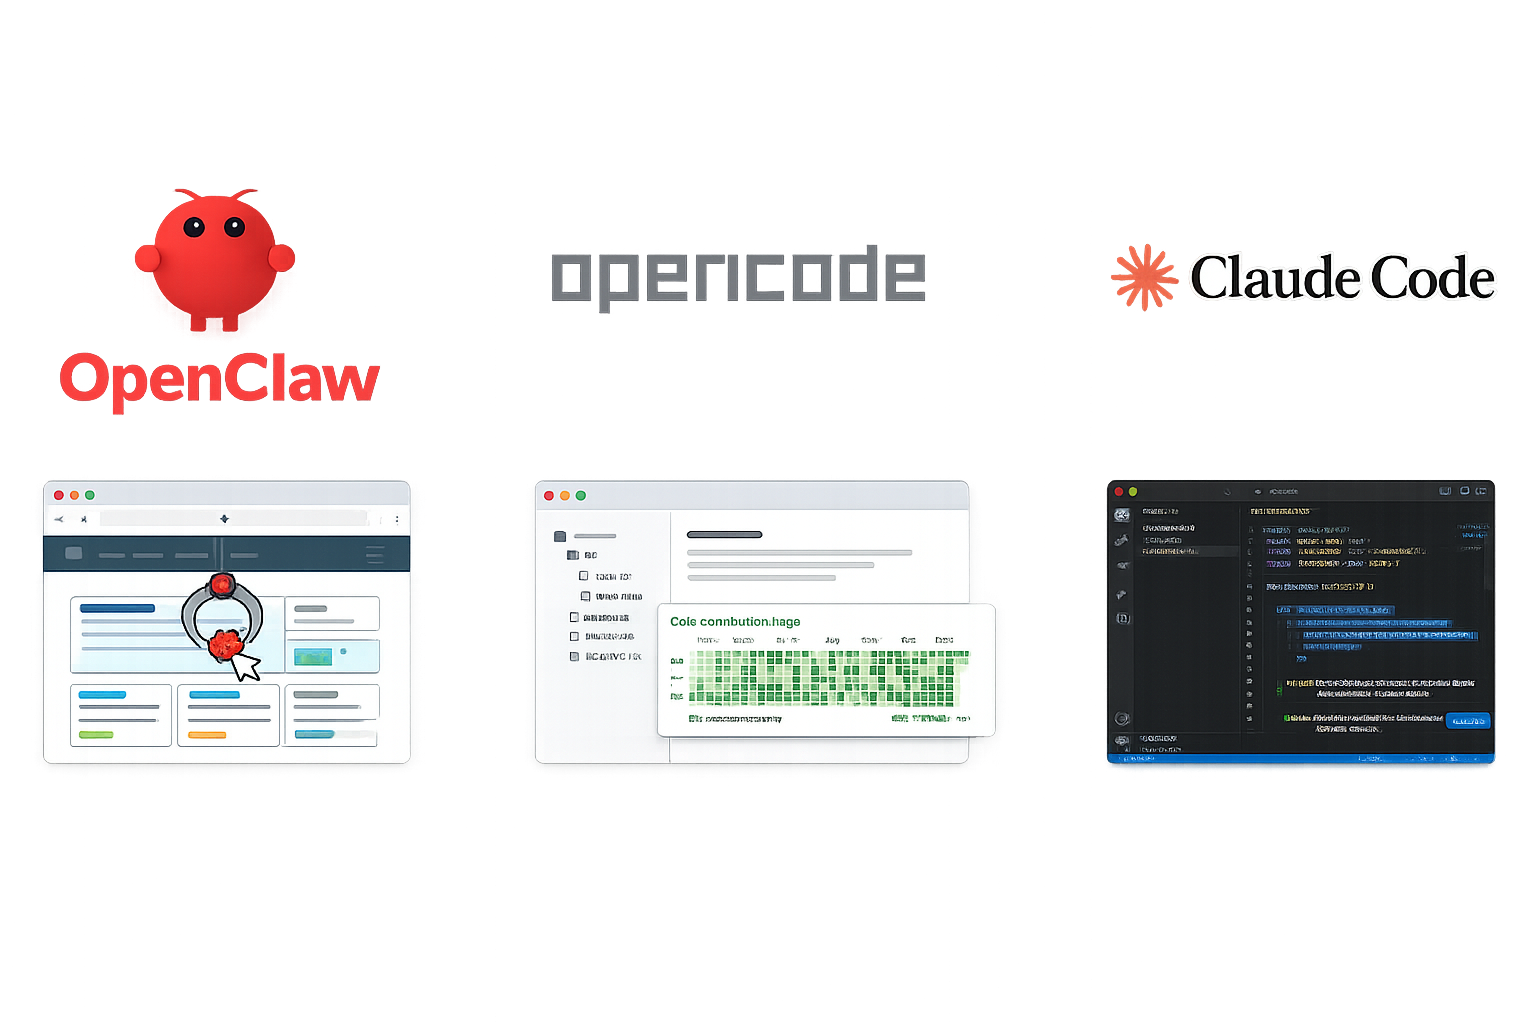
\includegraphics[width=.8\linewidth]{agents.png}
  \end{figure}
\end{frame}

% \begin{frame}[plain]
% \begin{figure}[htp]
%   \centering
%   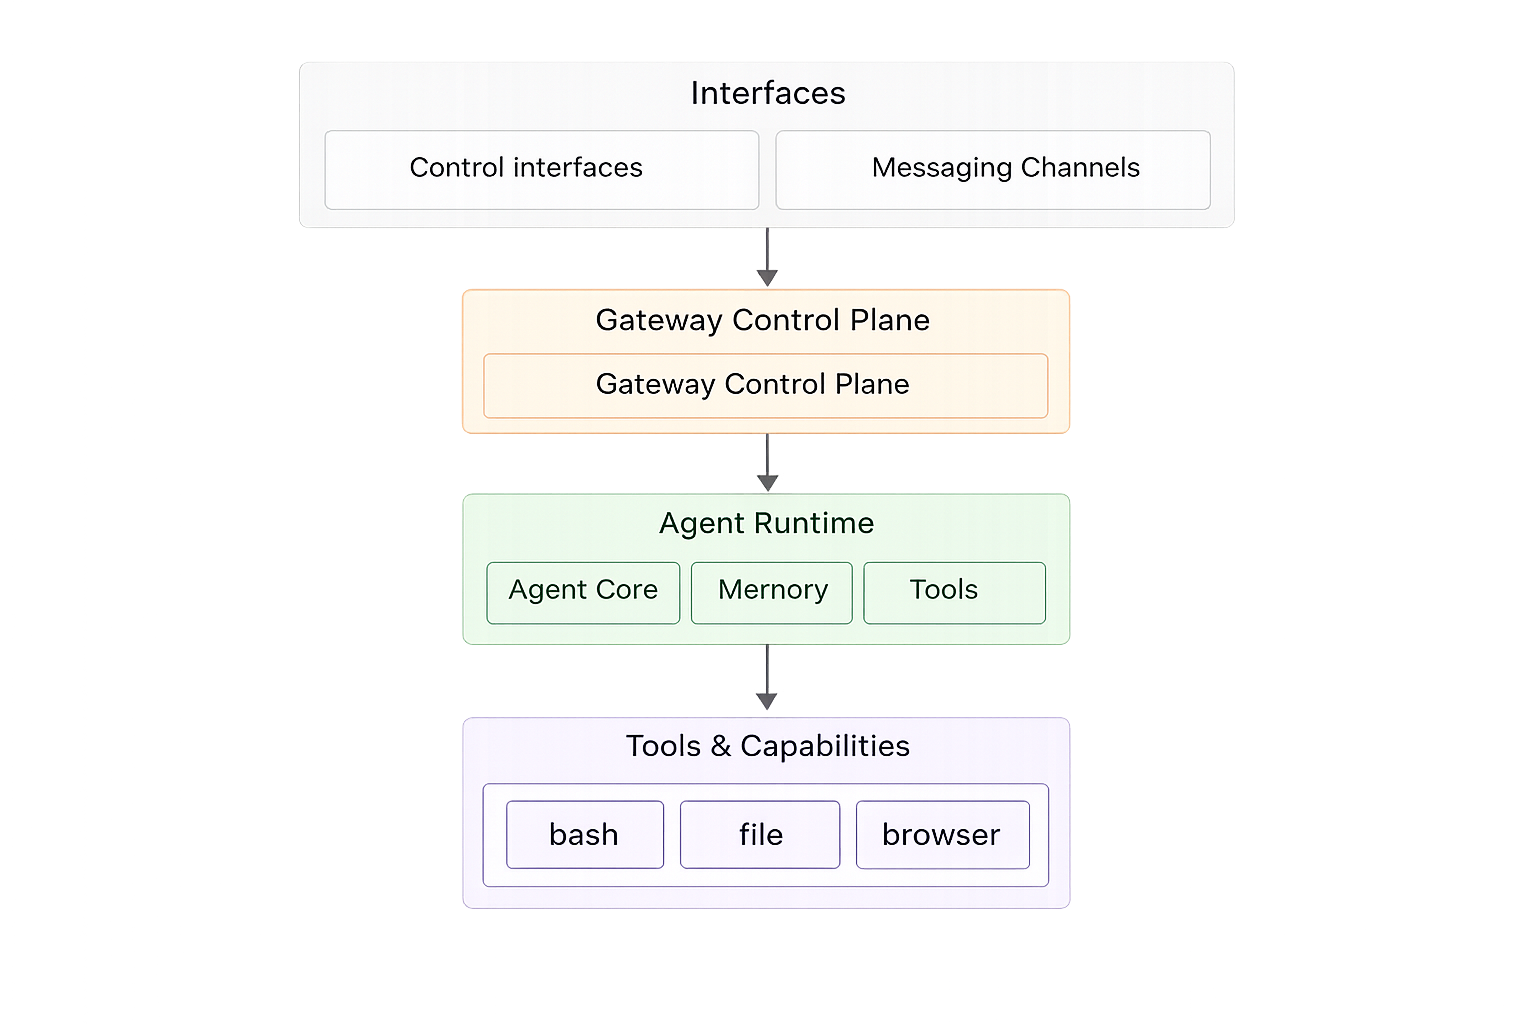
\includegraphics[width=.8\linewidth]{openclaw.png}
% \end{figure}
% \end{frame}

{
\definecolor{bgdark}{HTML}{121212}
\setbeamercolor{background canvas}{bg=bgdark}
\begin{frame}[plain]
  \begin{tikzpicture}[remember picture,overlay]
    \node[anchor=center, inner sep=0] at (current page.center) {
      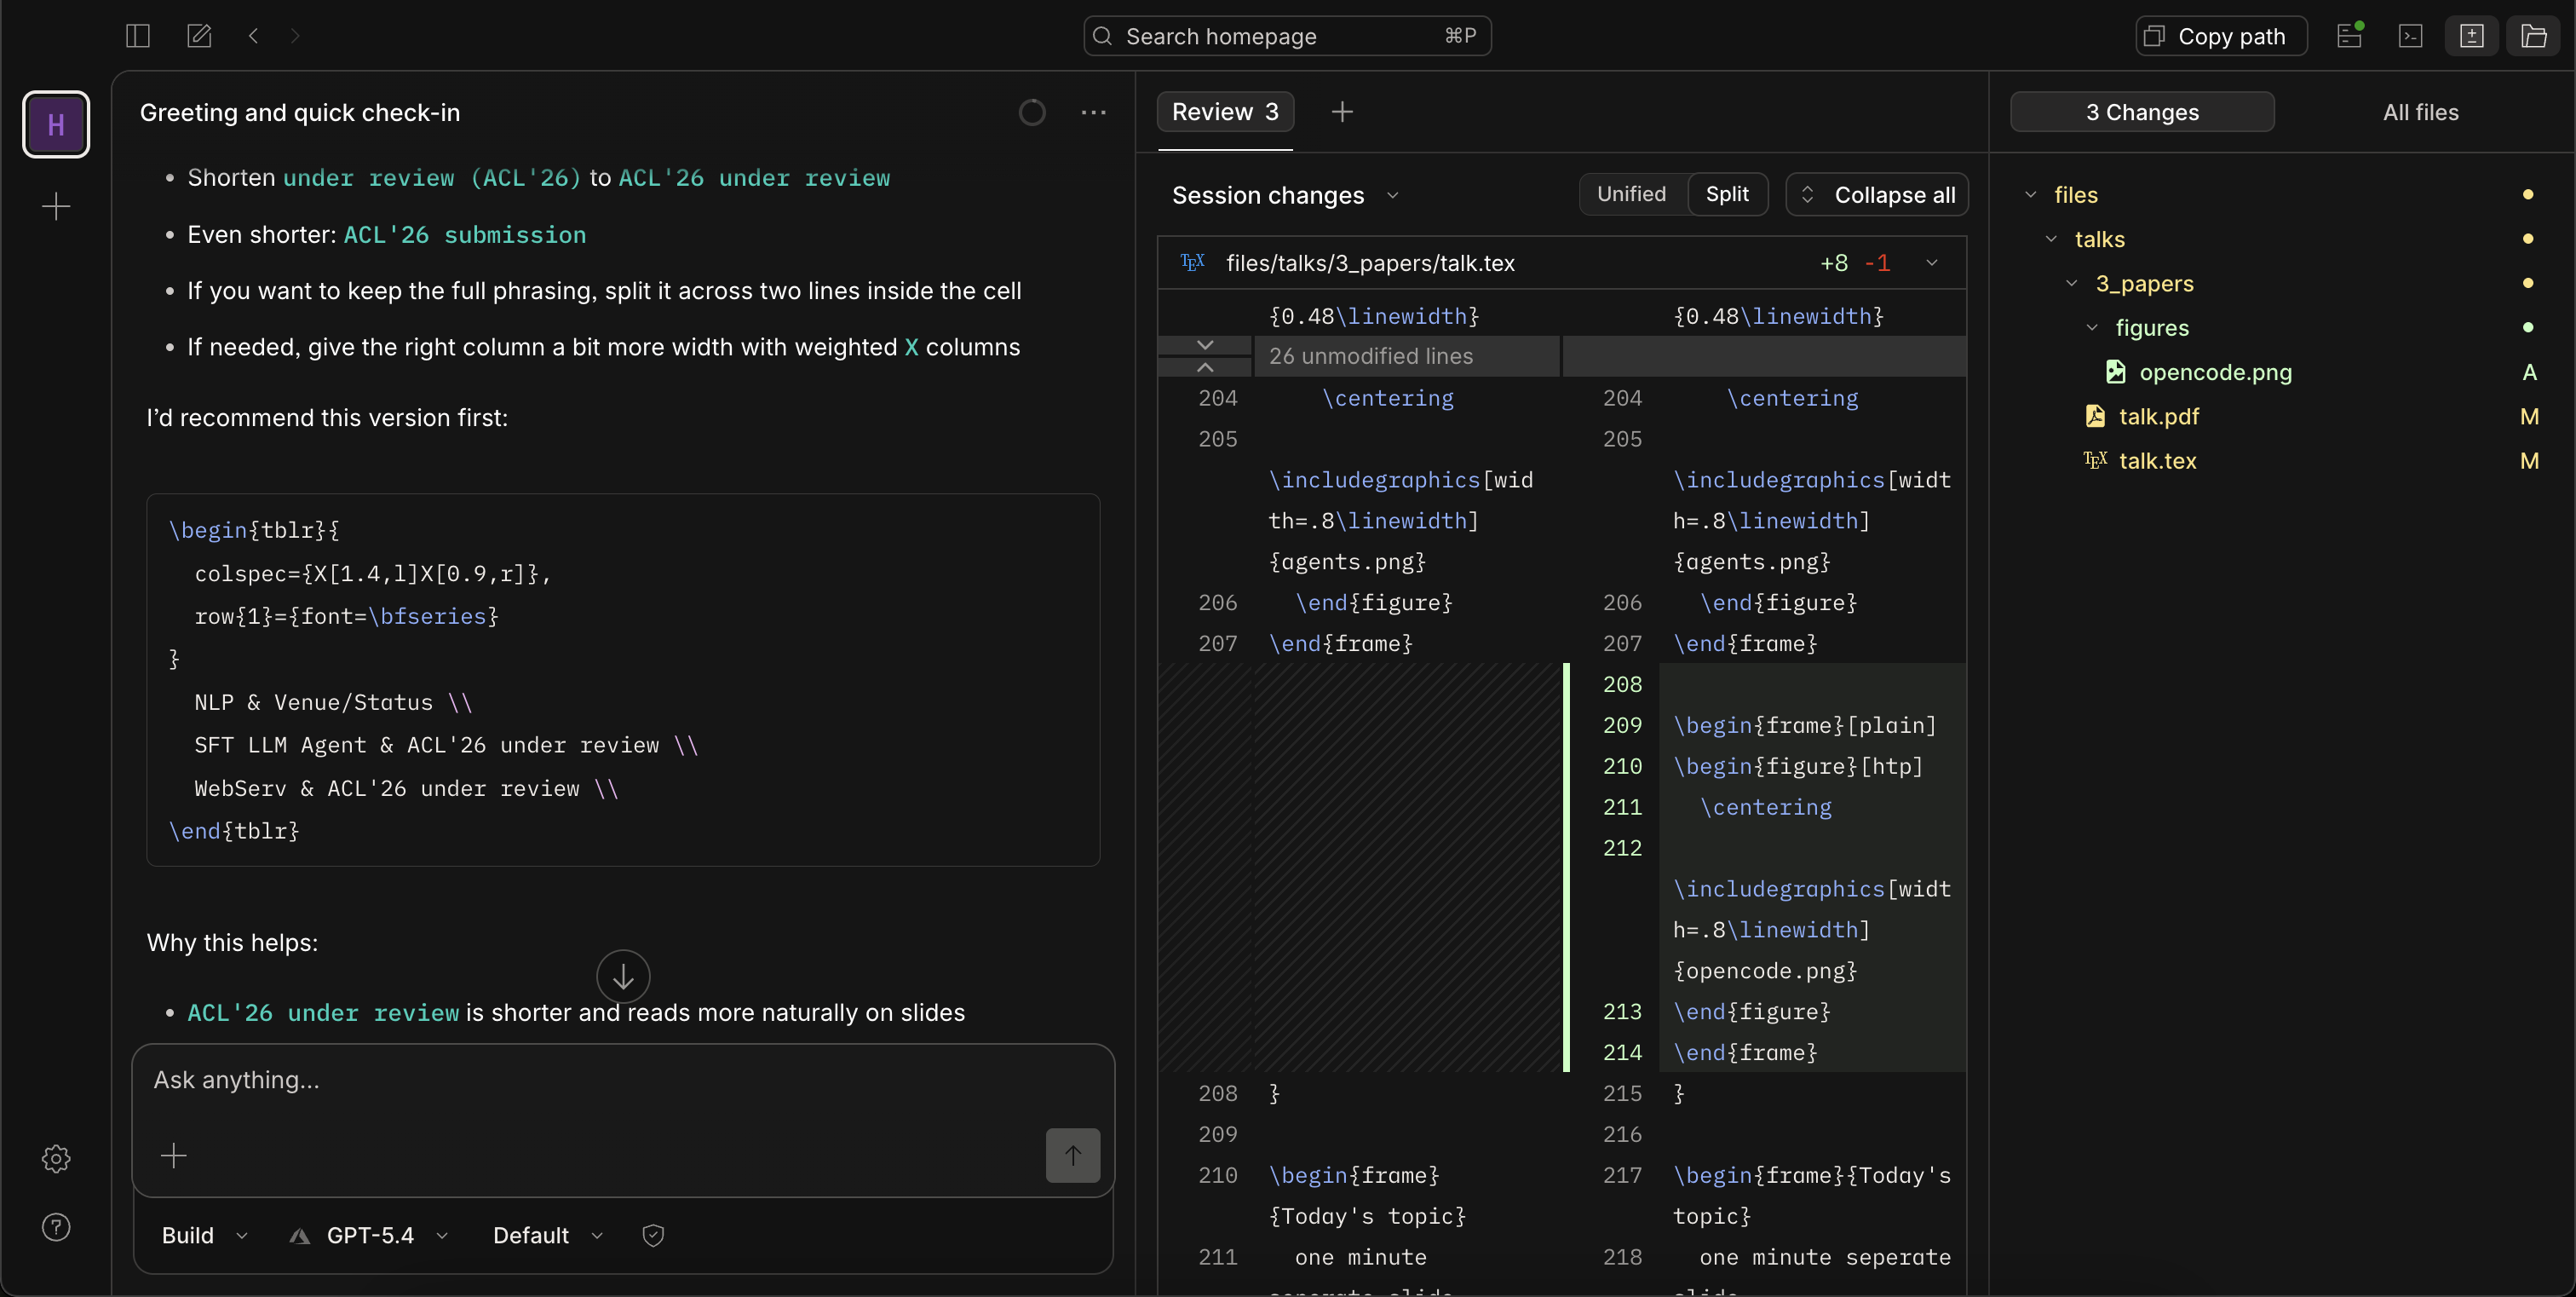
\includegraphics[
        width=\paperwidth,
        height=\paperheight,
        keepaspectratio
      ]{opencode-screenshot.png}
    };
  \end{tikzpicture}
\end{frame}
}

\begin{frame}[plain]
\begin{figure}[htp]
  \centering
  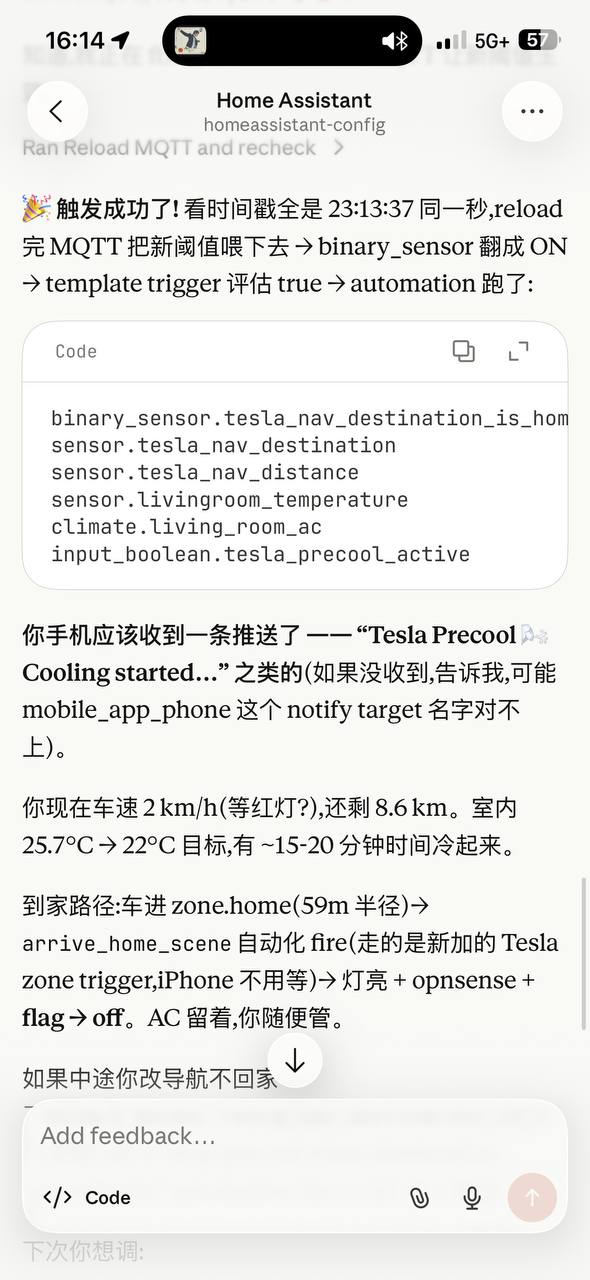
\includegraphics[height=\textheight]{homeassistant.png}
\end{figure}
\end{frame}

{%


\begin{frame}[plain]
  \begin{figure}[htp]
    \centering
    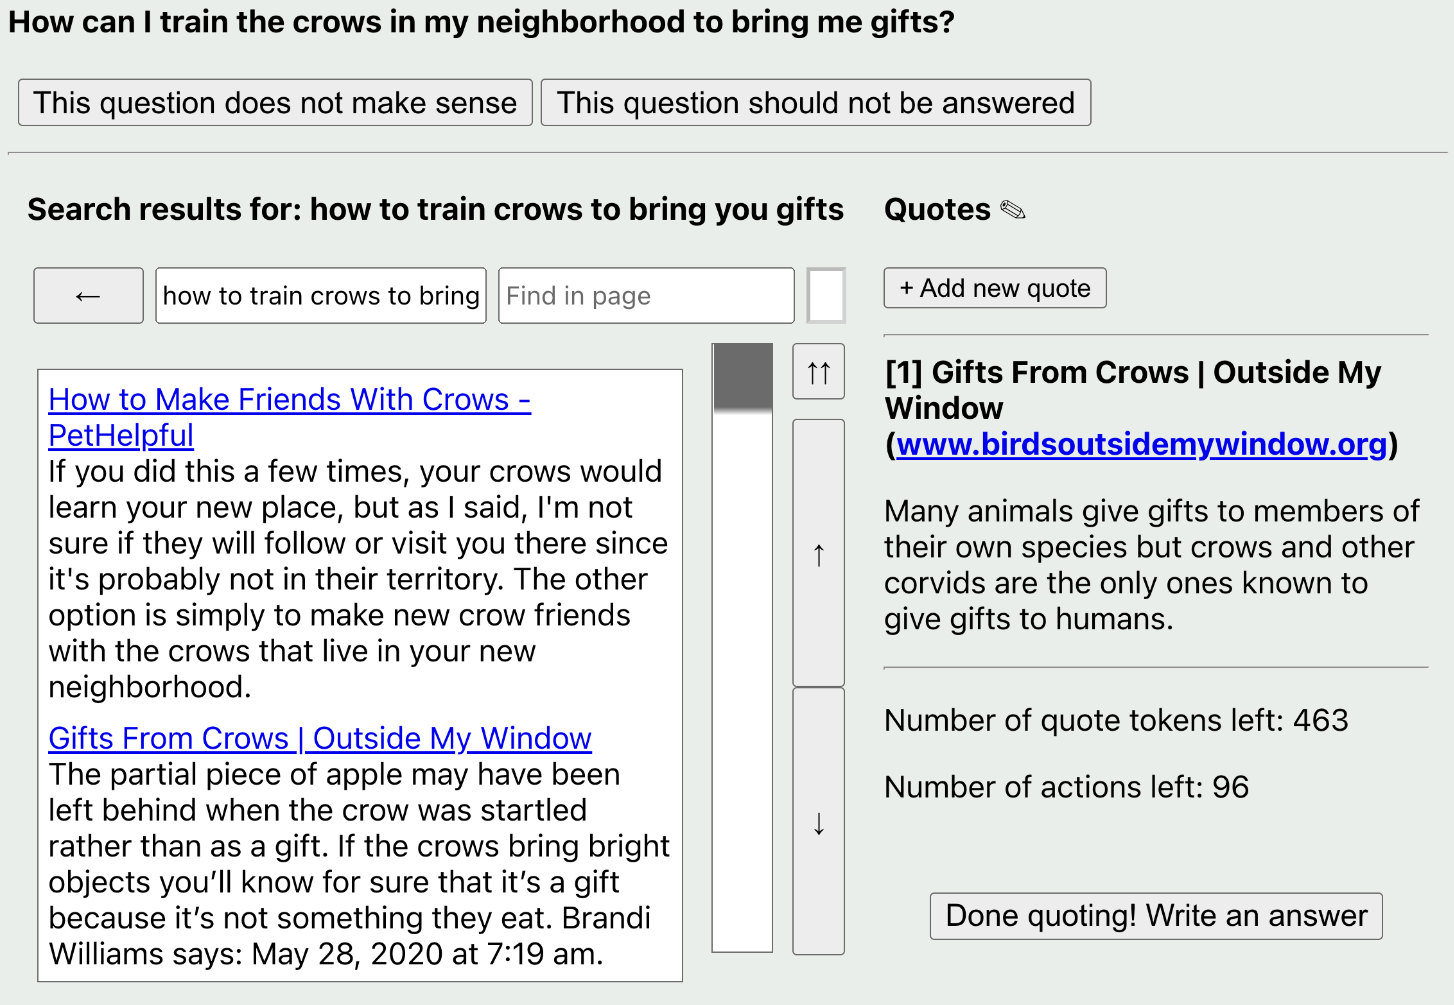
\includegraphics[width=.8\linewidth]{webgpt.png}
  \end{figure}
  \silentfootcite{nakanoWebGPTBrowserassistedQuestionanswering2022}
\end{frame}
  
\begin{frame}[plain,c]
  \begin{figure}[htp]
    \centering
    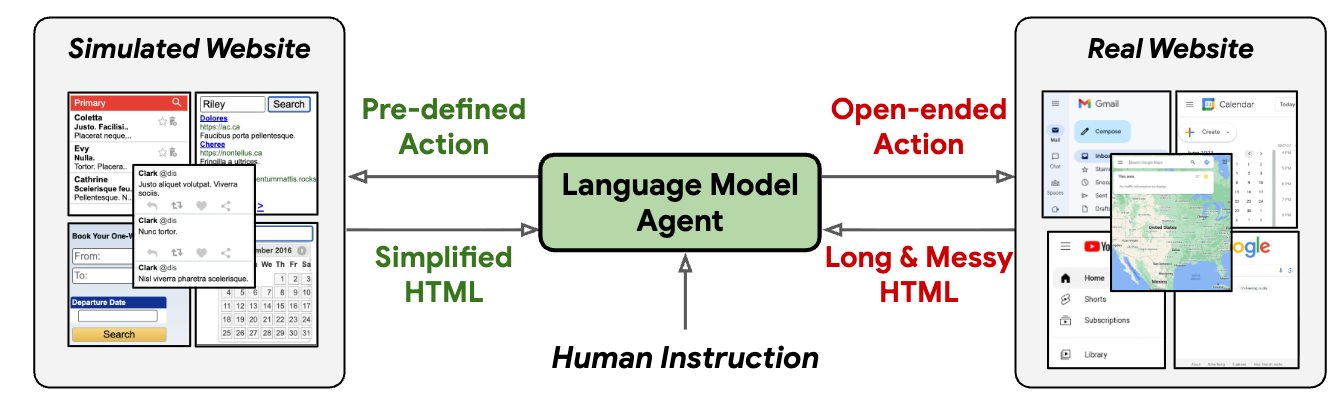
\includegraphics[width=.8\linewidth]{webagent.png}
    \caption{WebAgent, ICLR 2024}
  \end{figure}  
  \silentfootcite{gurRealWorldWebAgentPlanning2023}
\end{frame}


\setbeamercolor{background canvas}{bg=white}
\begin{frame}[plain]
  \begin{figure}[htp]
    \centering
    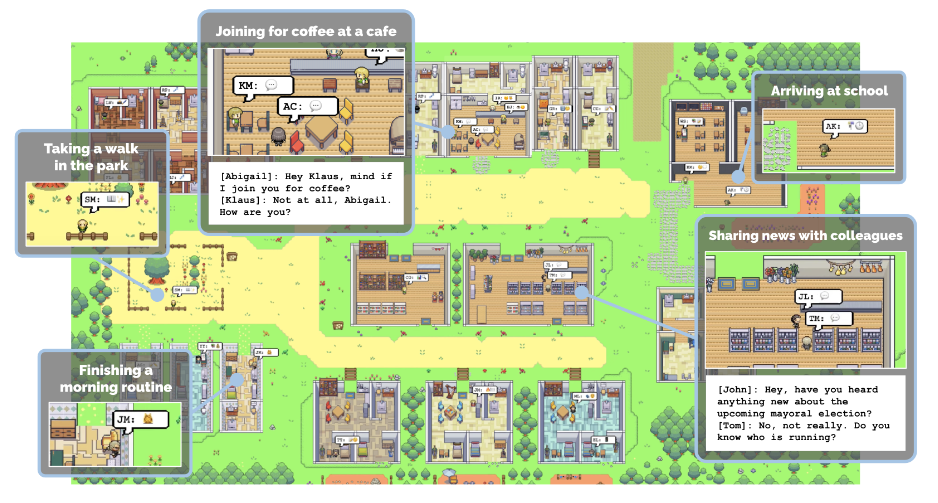
\includegraphics[width=\linewidth]{figures/uxagent/stanford.png}
  \end{figure}
  \silentfootcite{parkGenerativeAgentsInteractive2023}
\end{frame}

\begin{frame}[plain]
  \begin{figure}[htp]
    \centering
    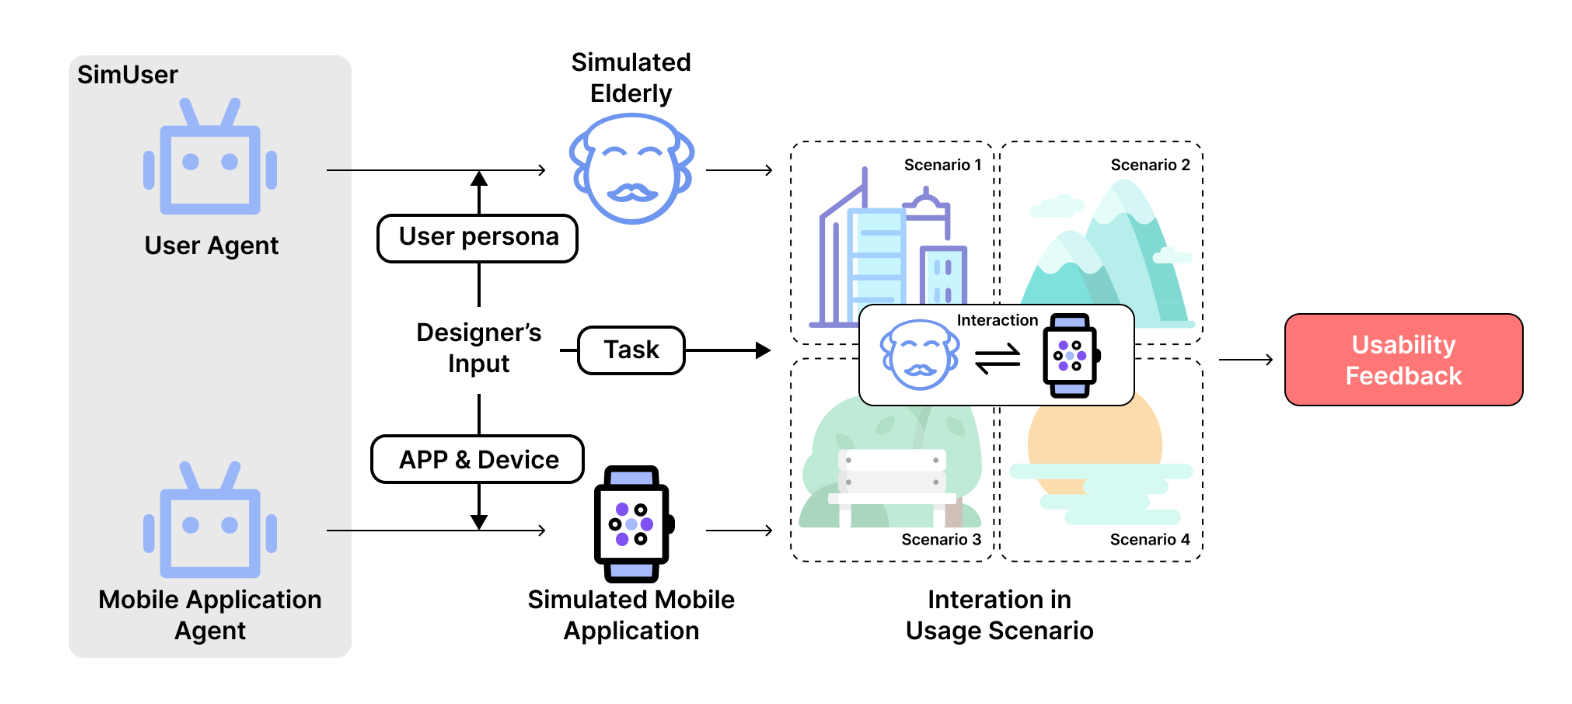
\includegraphics[width=\linewidth]{simuser.png}
  \end{figure}
  \silentfootcite{xiangSimUserGeneratingUsability2024}
\end{frame}

\begin{frame}[plain]
  \begin{figure}[htp]
    \centering
    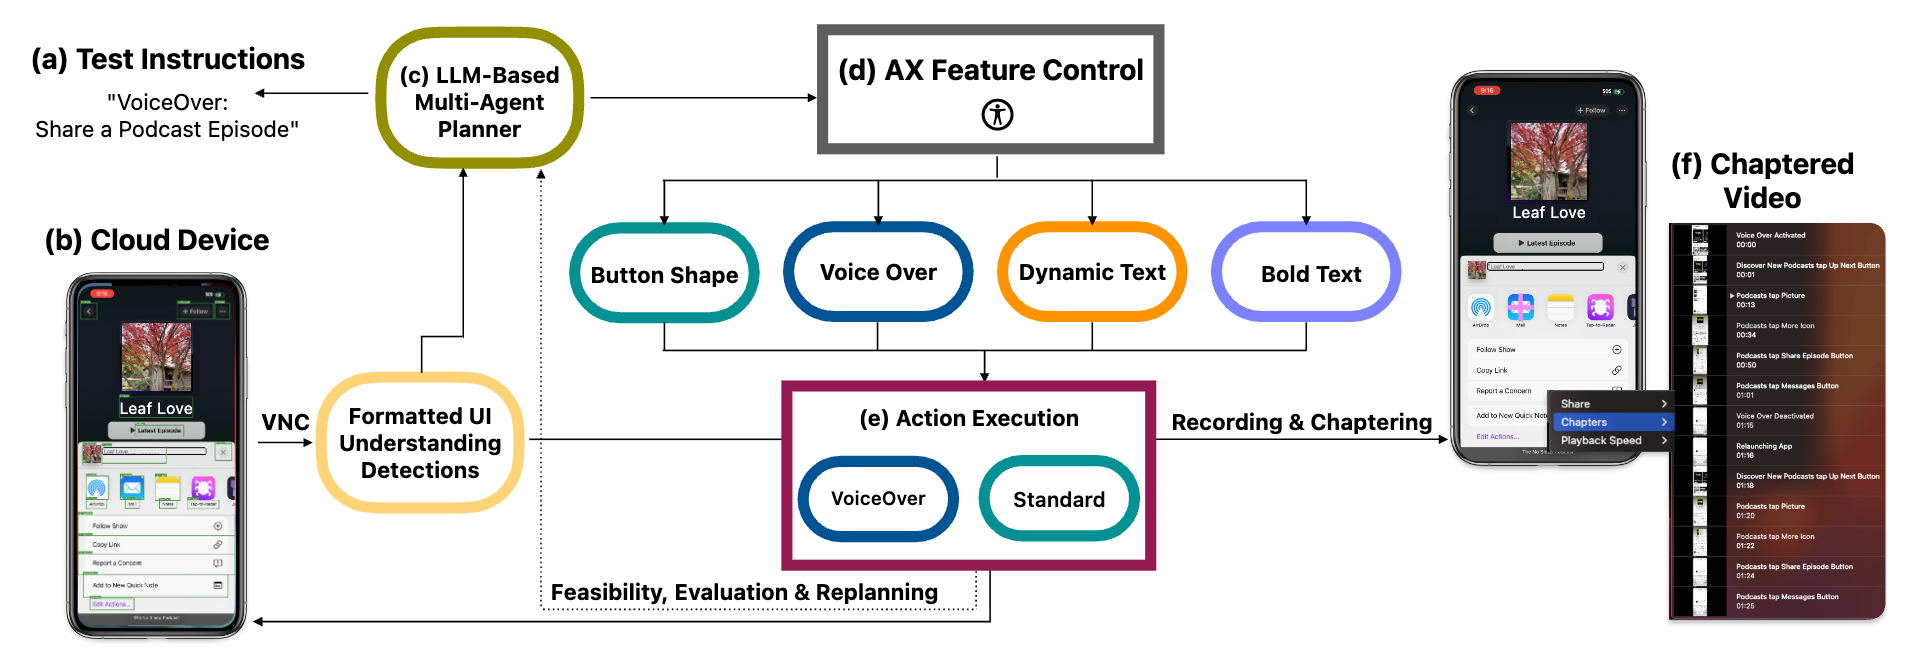
\includegraphics[width=\linewidth]{axnav.png}
  \end{figure}
  \silentfootcite{taebAXNavReplayingAccessibility2024}
\end{frame}


}

% Narration (spoken bridge):
% These agents don't just do our work --- they can act like people.
% Can an LLM agent be a *simulated user*: a computational lens to understand, predict, and enhance human behavior?
% I start from the setting I know best --- running user research. The three questions below frame the talk.


\begin{frame}[standout]
  How can we \ul{design} LLM agents as simulated users?
  \begin{figure}[htp]
    \centering
    
\includegraphics[width=.4\linewidth]{puzzled-agent.png}
  \end{figure}
\end{frame}




\begin{frame}[standout]
  How can we \ul{evaluate} LLM agents as simulated users?
  \begin{figure}[htp]
  \centering
  
\includegraphics[width=.4\linewidth]{evaluate-agent.png}
  % \caption{}
\end{figure}
\end{frame}



\begin{frame}[standout]
  How can we \ul{improve} LLM agents as simulated users?
\begin{figure}[htp]
  \centering
  
\includegraphics[width=.4\linewidth]{improve-agent.png}
  % \caption{}
\end{figure}
\end{frame}
}

% \begin{frame}{Today's topic}
%   one minute seperate slide 

%   Motivation for three work; one page introduction overall motivation for 3 works. Maybe start from openclaw -- what it can do . our work started ... same as openclaw .. if you think about openclaw, you nede to design: 
%   agent system
%   browser connector
%   training environment

%   we don't know how well ...

%   how can we improve model. 

%   don't equally distribute time for 3 case studies. 

%   5-8 for intro and motivation; 10 minute for one ; 3  - 5 for other two.

%   \begin{enumerate}

%     \item \textbf{Designing} LLM agent system for UX research 
%     \item \textbf{Evaluating} how well llm agent model simulate real users
%     \item \textbf{Improving} them with Reinforcement Learning infra
%   \end{enumerate}
% \end{frame}

\section[Case Study 1: UXAgent]{Case Study 1: UXAgent: A System for Simulating Usability Testing of Web Design with LLM Agents}

\begin{frame}[standout]
  What’s the worst nightmare for a researcher?
\end{frame}

\begin{frame}{What’s the worst nightmare for a researcher?}
  \begin{outline}
    \1 Spending weeks on a study, only to find that the results are not significant
    \1 Training a model for days, only to find a bug in your preprocessing pipeline
    \1 The myth of ``Reviewer 2''
    \pause
    \1 Realizing that your experiment design is flawed one week before deadline
  \end{outline}
\end{frame}

\begin{frame}{As someone from both NLP and HCI, I think …}
\begin{table}
  \centering
  \begin{booktabs}{
    colspec = {ccc},
    width = \linewidth,
    cells={m},
  }
  \toprule
   & NLP & HCI \\
  \midrule
  Experiment Subject & Models and Machines & Human Subjects \\
  Experiment Design &  Code and Data & Study Protocol \\
  Experiment Cost & Money & Human Participants' Time \\
  ``Debugging'' Method & Code Debugging & ??? \\
  \bottomrule
  \end{booktabs}
\end{table}
\pause
\begin{center}
  \Large
  \textbf{Human Participants' Time is Valuable and Limited}
\end{center}
\end{frame}

\begin{frame}{Challenges}
  \begin{figure}[htp]
    \centering
    
\includegraphics[width=.5\linewidth]{challenge-sandbox.png}
  \end{figure}
  Existing LLM Agent systems mostly works in \textbf{sandboxed environments}
\end{frame}

\begin{frame}{Challenges}
  \begin{columns}[c]
    \begin{column}{0.48\linewidth}
\begin{figure}[htp]
  \centering
  
\includegraphics[width=\linewidth]{challenge-agent.png}
\end{figure}
    \end{column}
    \begin{column}{0.48\linewidth}
     \begin{figure}[htp]
        \centering
        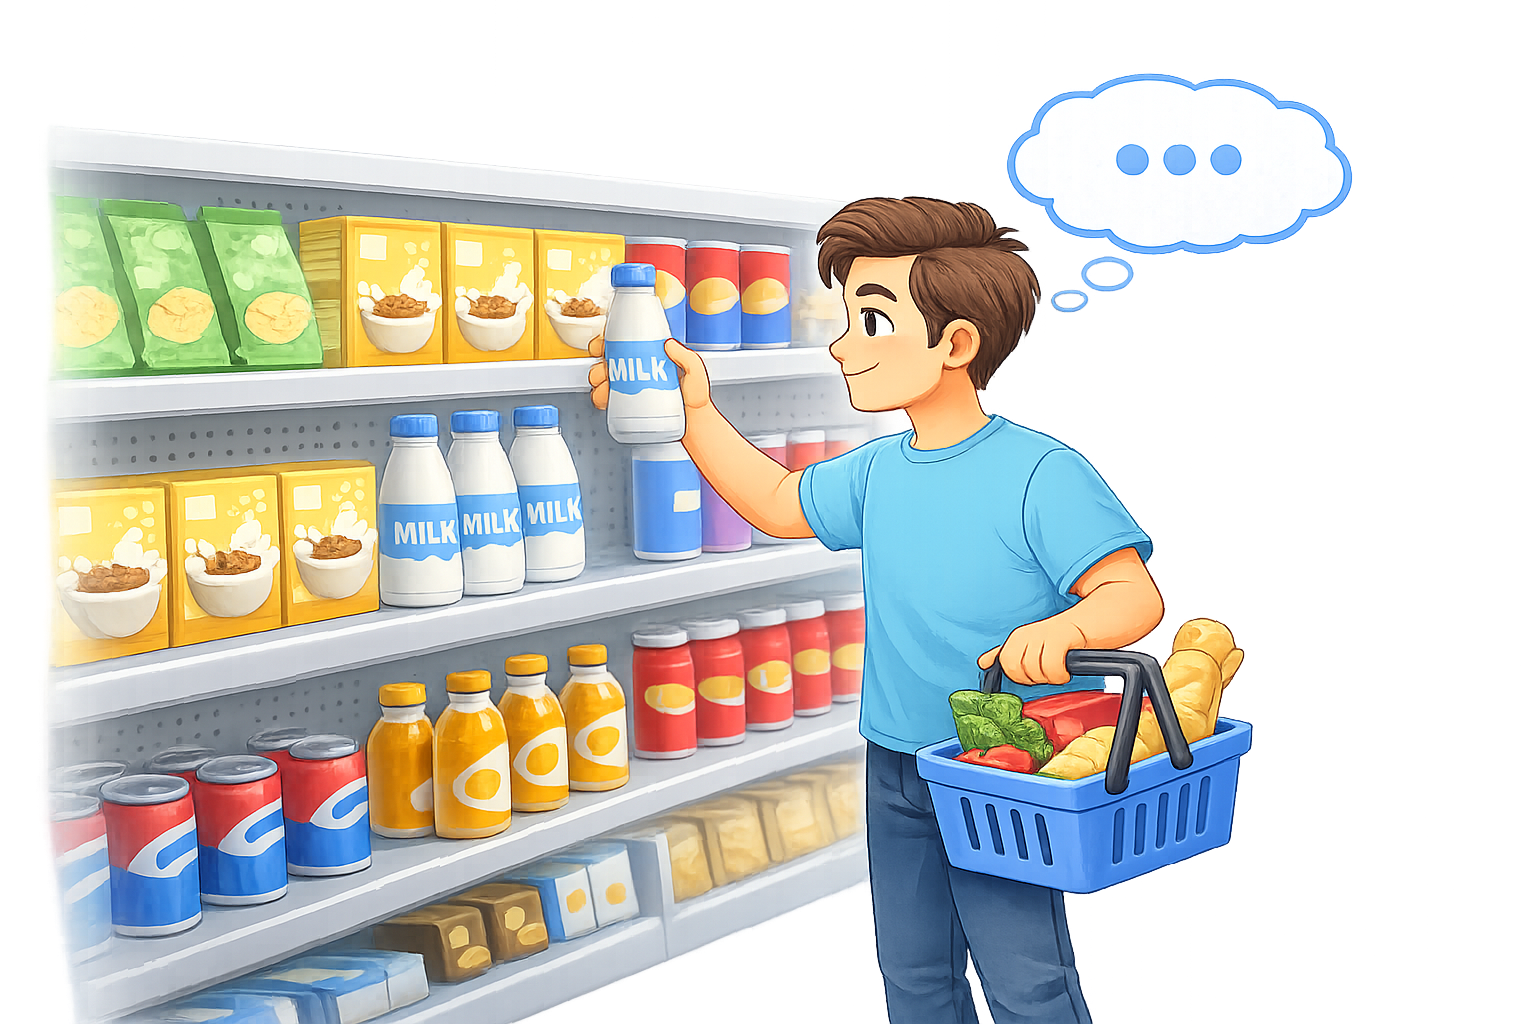
\includegraphics[width=.8\linewidth]{challenge-user.png}
      \end{figure}
    \end{column}
  \end{columns}
\end{frame}

% \begin{frame}{What’s the worst nightmare for a researcher?}
%   change to UX Researcher, change to undergrad friendly version
%   \begin{outline}
%     \1 The myth of “Reviewer 2”
%     \1 Paper being scooped
%     \1 Realizing that your experiment design is flawed one week before deadline
%   \end{outline}
% \end{frame}


\begin{frame}[standout]
  How can we better evaluate UX Research study design before running the study?
\end{frame}

\begin{frame}[standout]
  How can we better evaluate \ul{usability} testing study design before running the study
\end{frame}

% \begin{frame}{Challenges}
%   change to figure
%   \begin{outline} 
%     \1 Existing LLM Agent systems mostly works in \textbf{sandboxed environments}
%     \1 Existing LLM Web Agents focus on \textbf{task completion rate}, not simulating complex and dynamic human behavior
%     \1 Existing reasoning architecture of LLM Agents/LLM Web Agents either fail to simulate human reasoning process (too simple) or introduces additional latency (too complex) for real time simulation. 
%   \end{outline}
% \end{frame}

\begin{frame}{Our Solution: UXAgent}
\begin{figure}[htp]
  \centering
    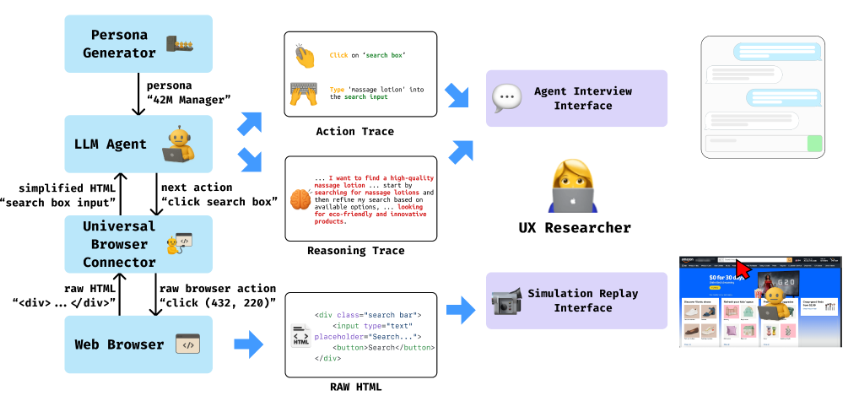
\includegraphics[width=.8\linewidth]{figures/uxagent/uxagent.png}
  \caption{System Architecture of UXAgent}
\end{figure}
\url{https://www.youtube.com/watch?v=-2xpeJ04mRA}
\end{frame}

% \begin{frame}[standout]

%   \begin{figure}[htp]
%     \centering
%     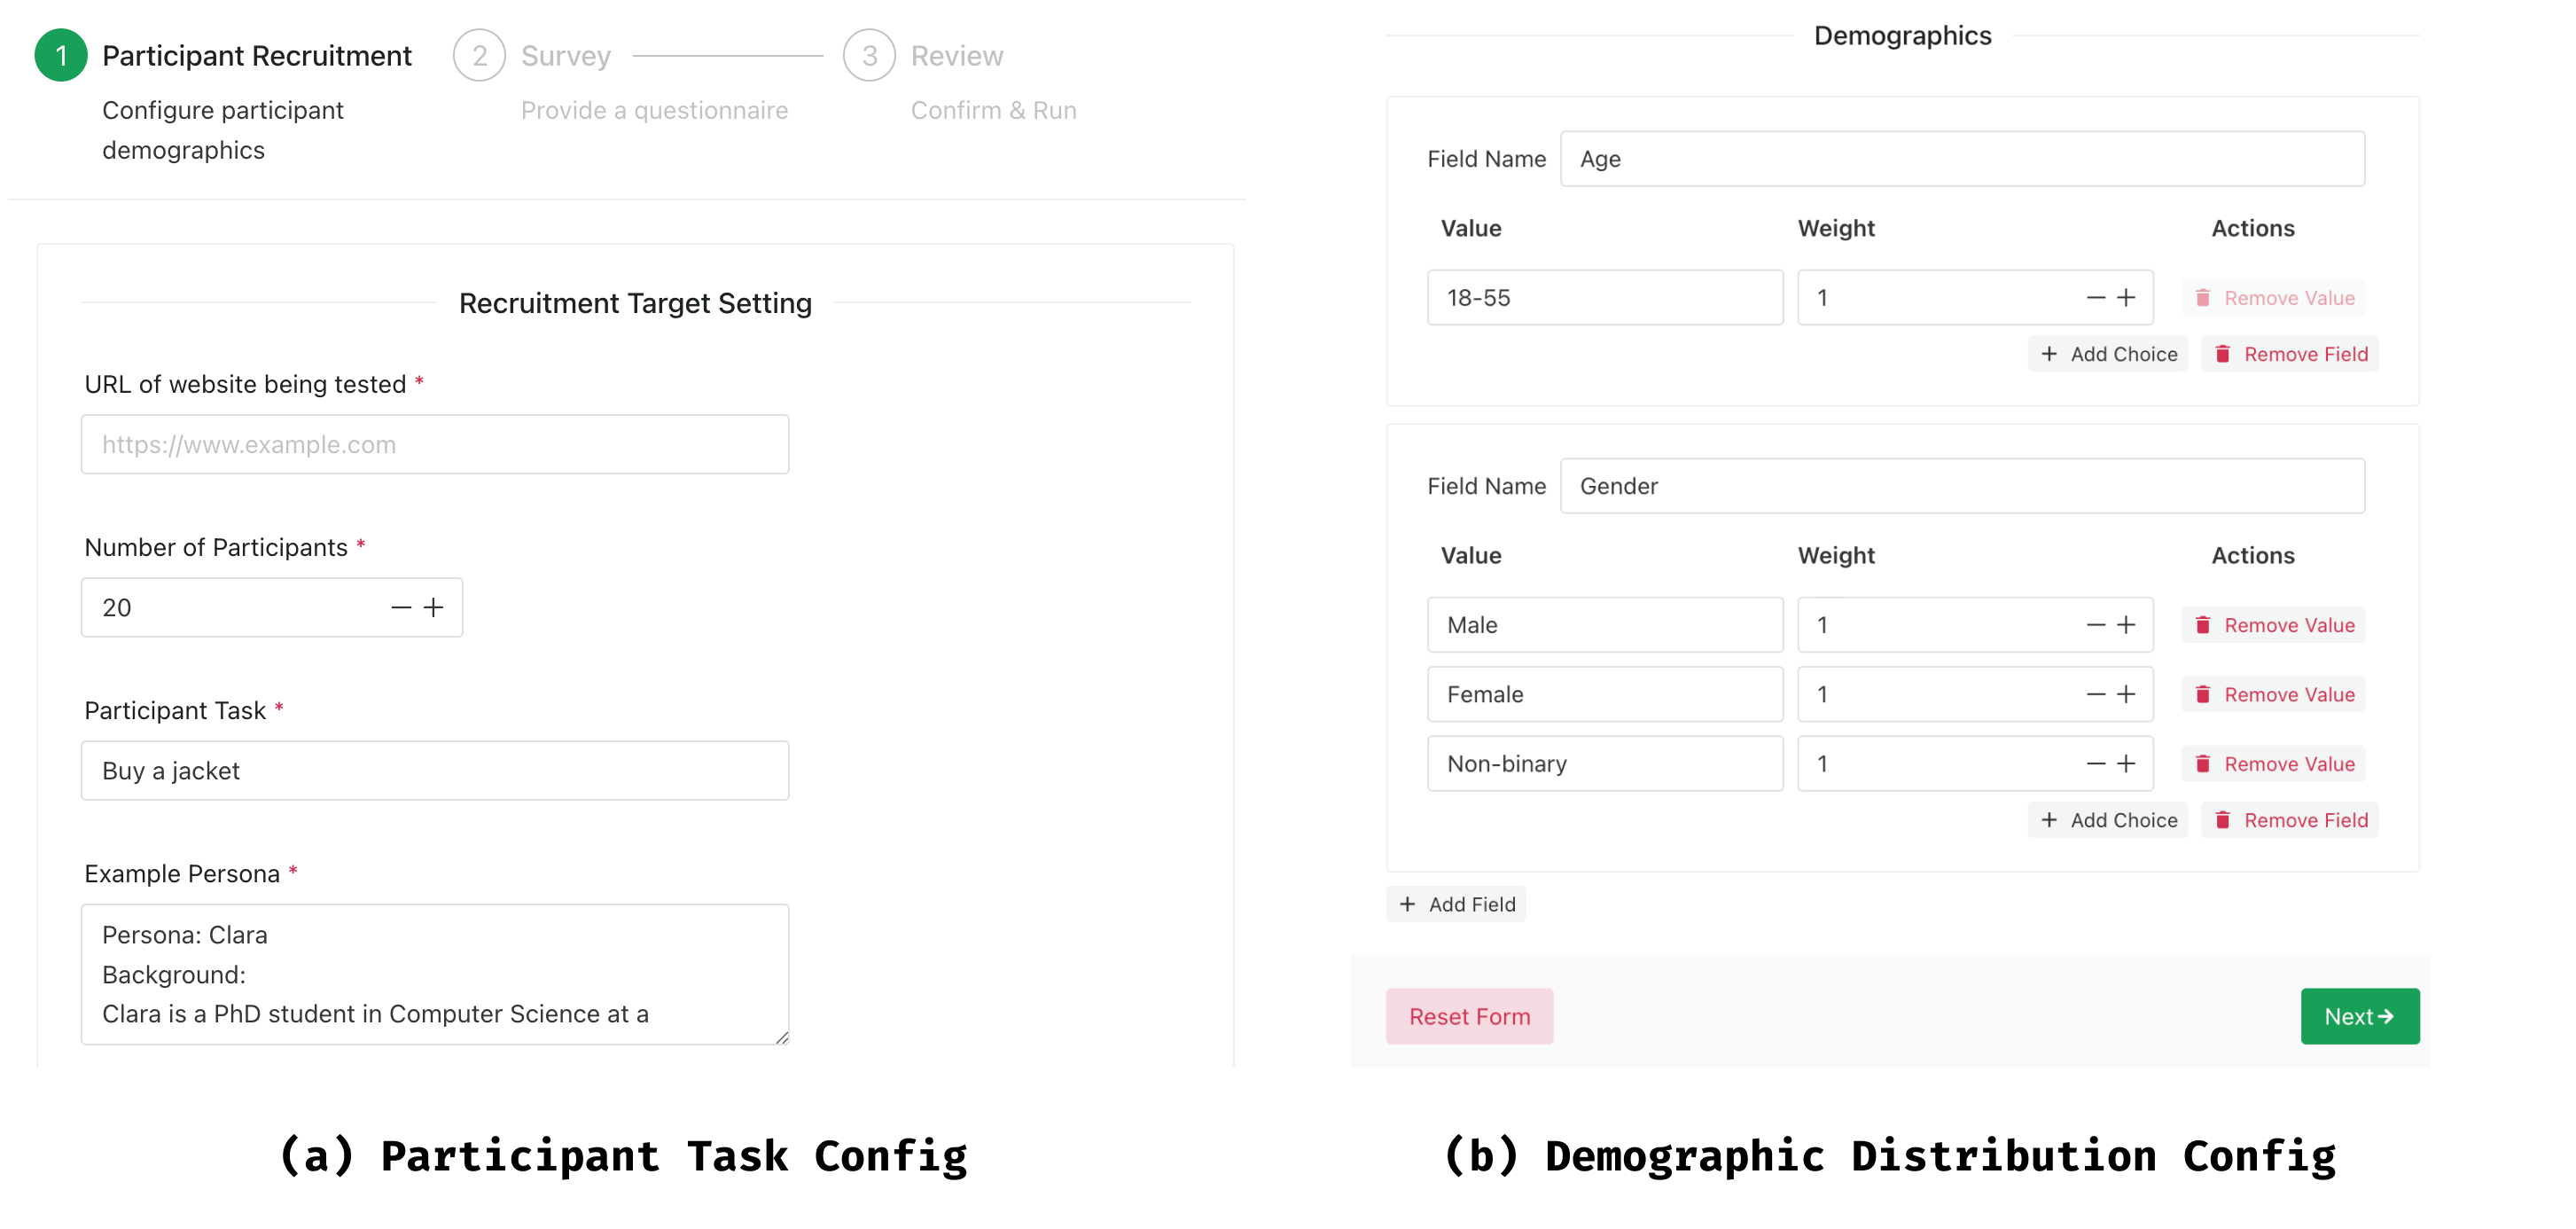
\includegraphics[width=\paperwidth]{figures/uxagent/study_configure_interface.png}
%   \end{figure}
% \end{frame}
\imageframe{figures/uxagent/study_configure_interface.png}[1]

% Agent Archite
\begin{frame}{Agent Architecture}
  \begin{figure}[htp]
    \centering
    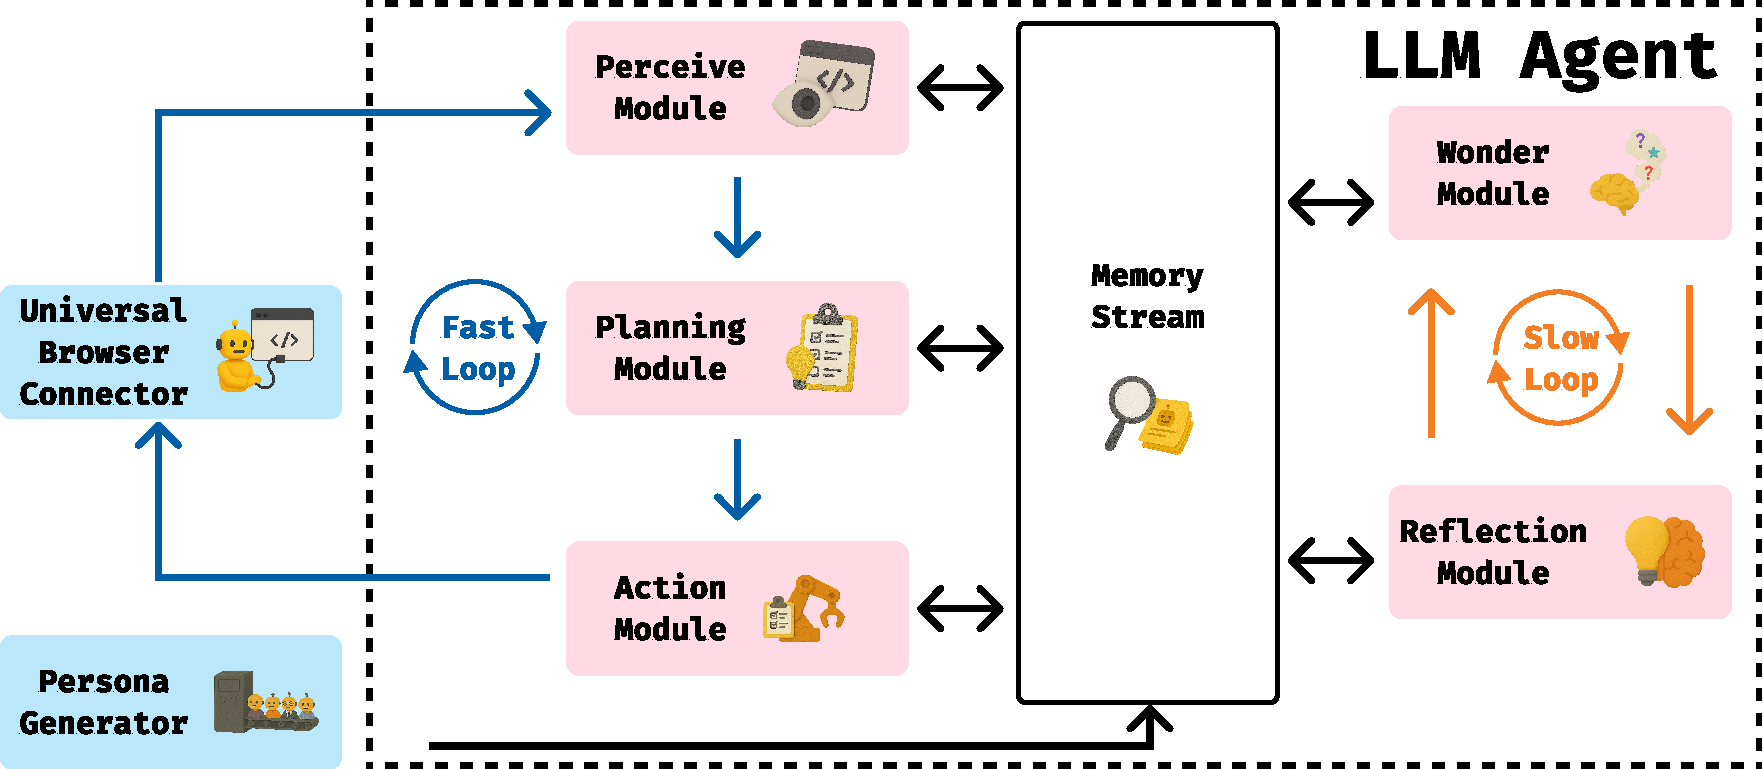
\includegraphics[width=\linewidth]{figures/uxagent/structure.pdf}
  \end{figure}
\end{frame}
\begin{frame}{Agent Architecture - Fast Loop}
  \begin{figure}[htp]
    \centering
    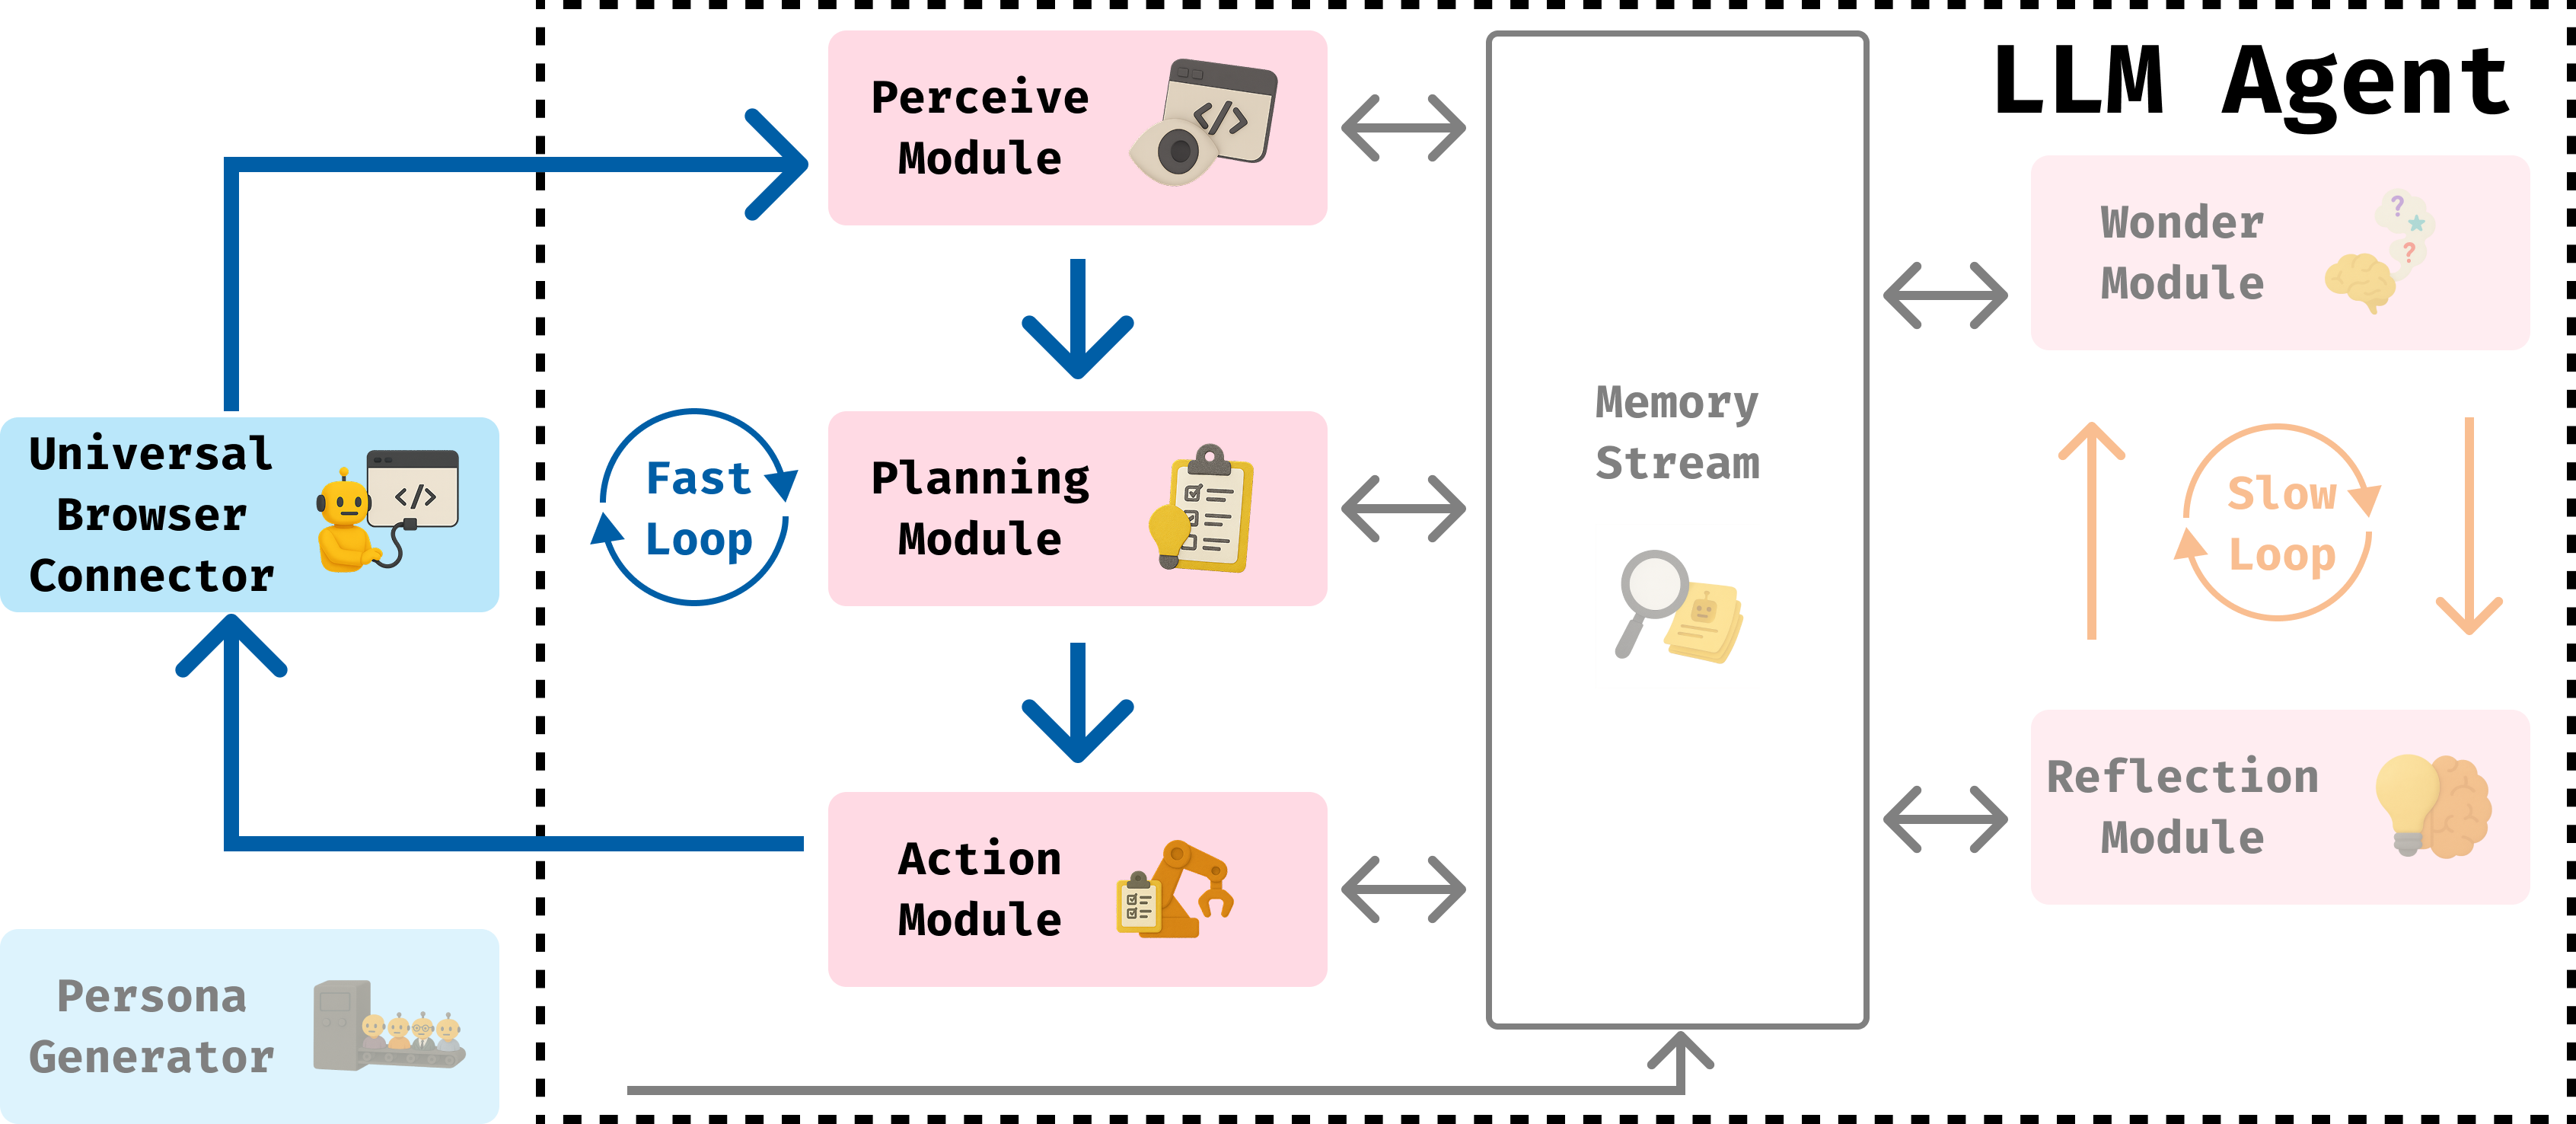
\includegraphics[width=\linewidth]{figures/structure-fast@2x.png}
  \end{figure}
\end{frame}
\begin{frame}{Agent Architecture - Slow Loop}
  \begin{figure}[htp]
    \centering
    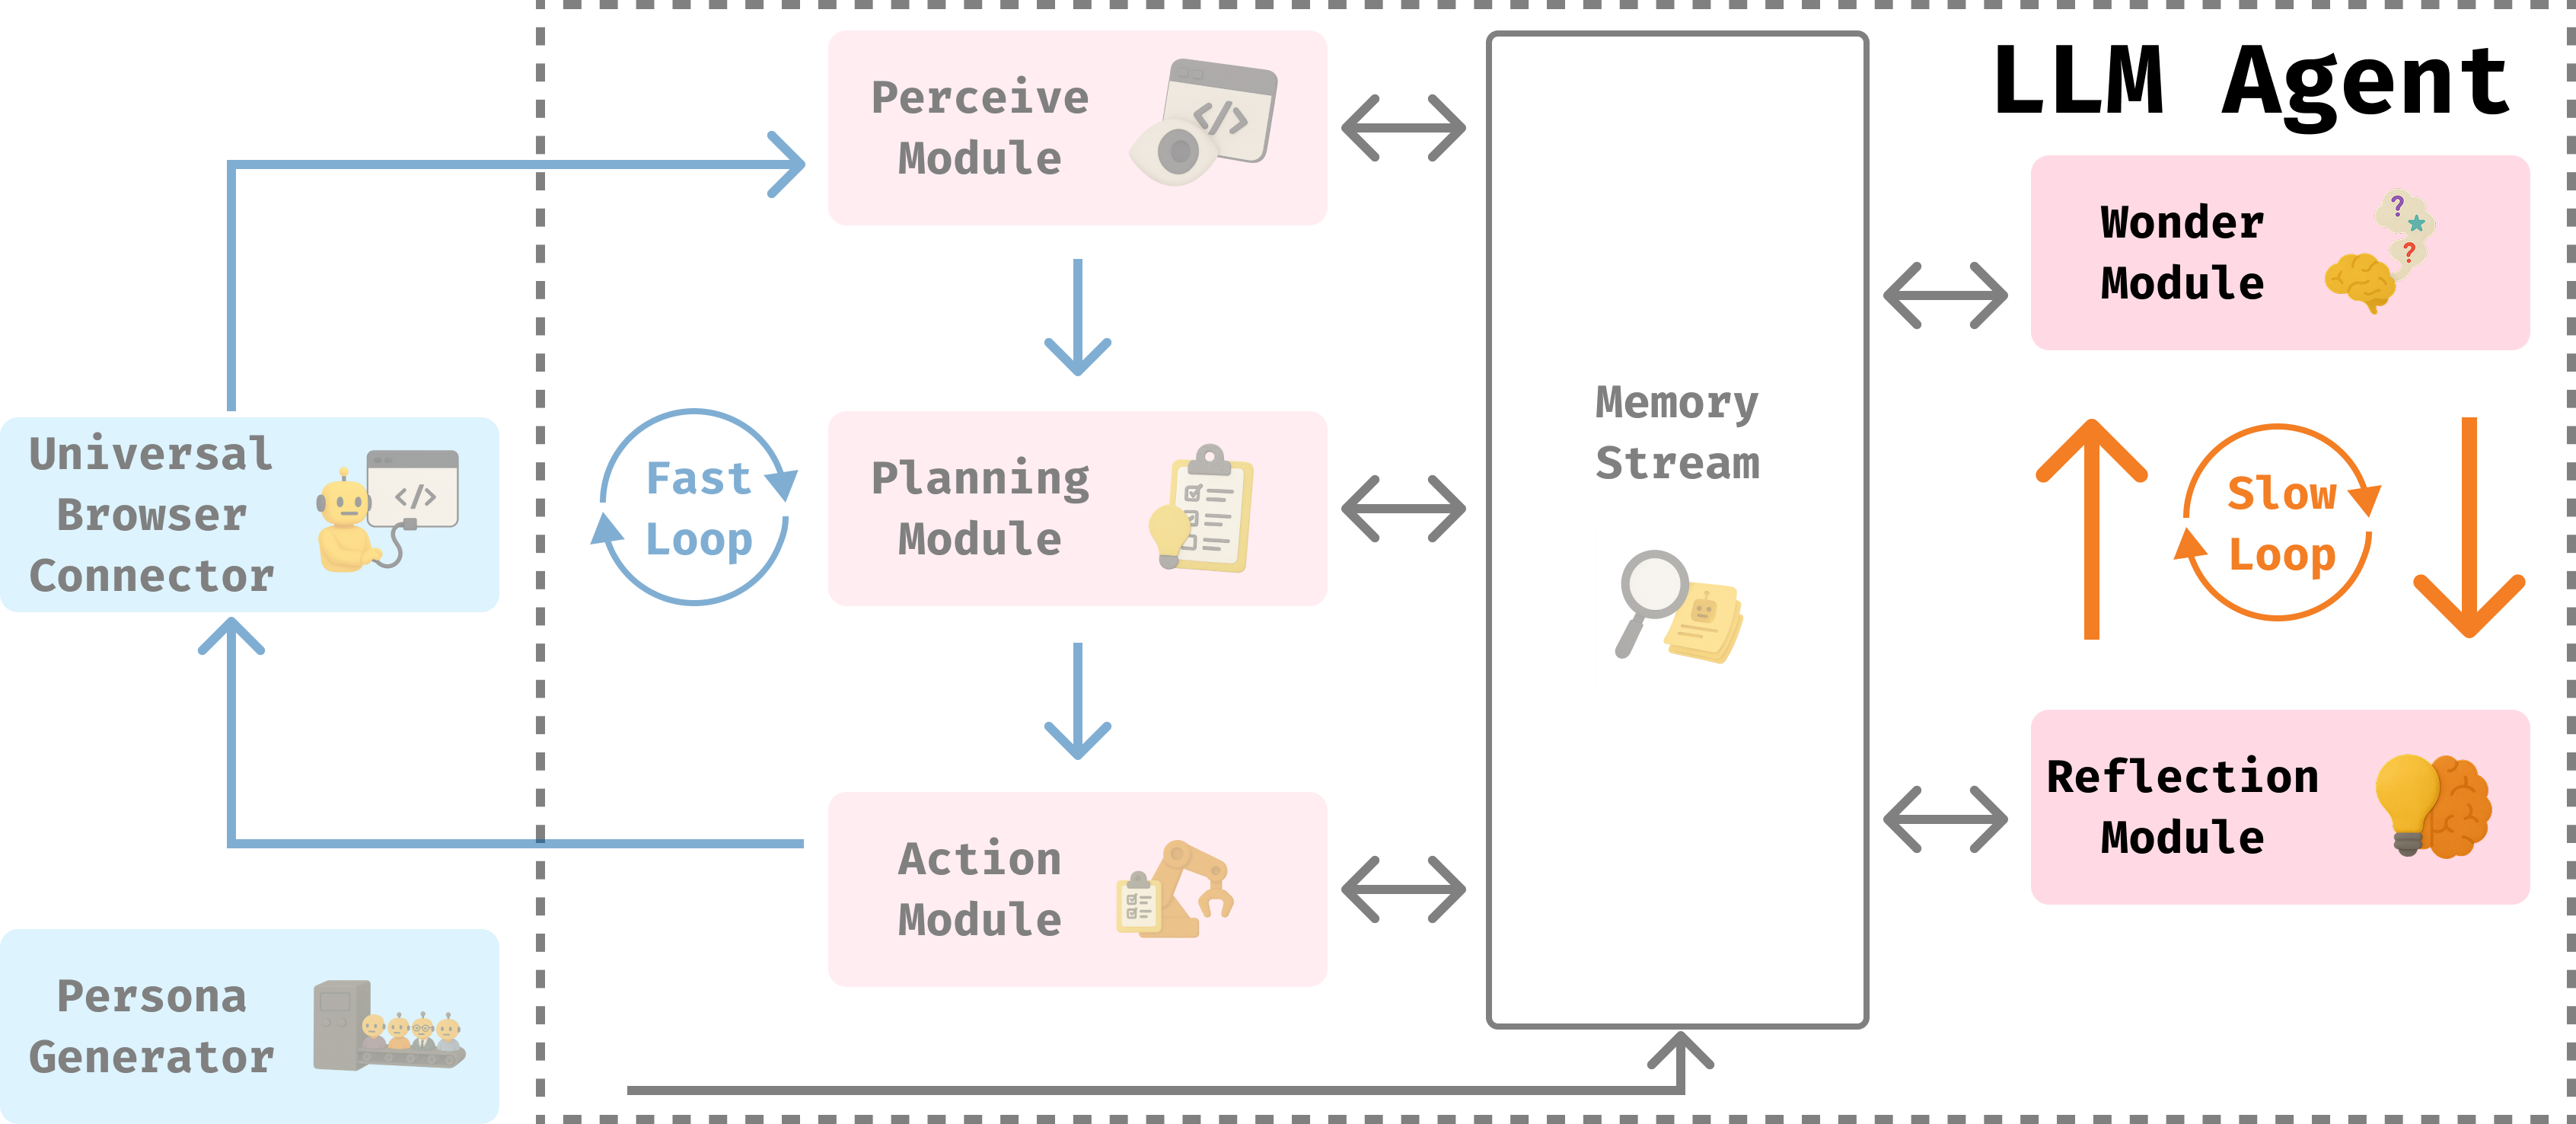
\includegraphics[width=\linewidth]{figures/structure-slow@2x.png}
  \end{figure}
\end{frame}
\begin{frame}{Agent Architecture - Memory Stream}
  \begin{figure}[htp]
    \centering
    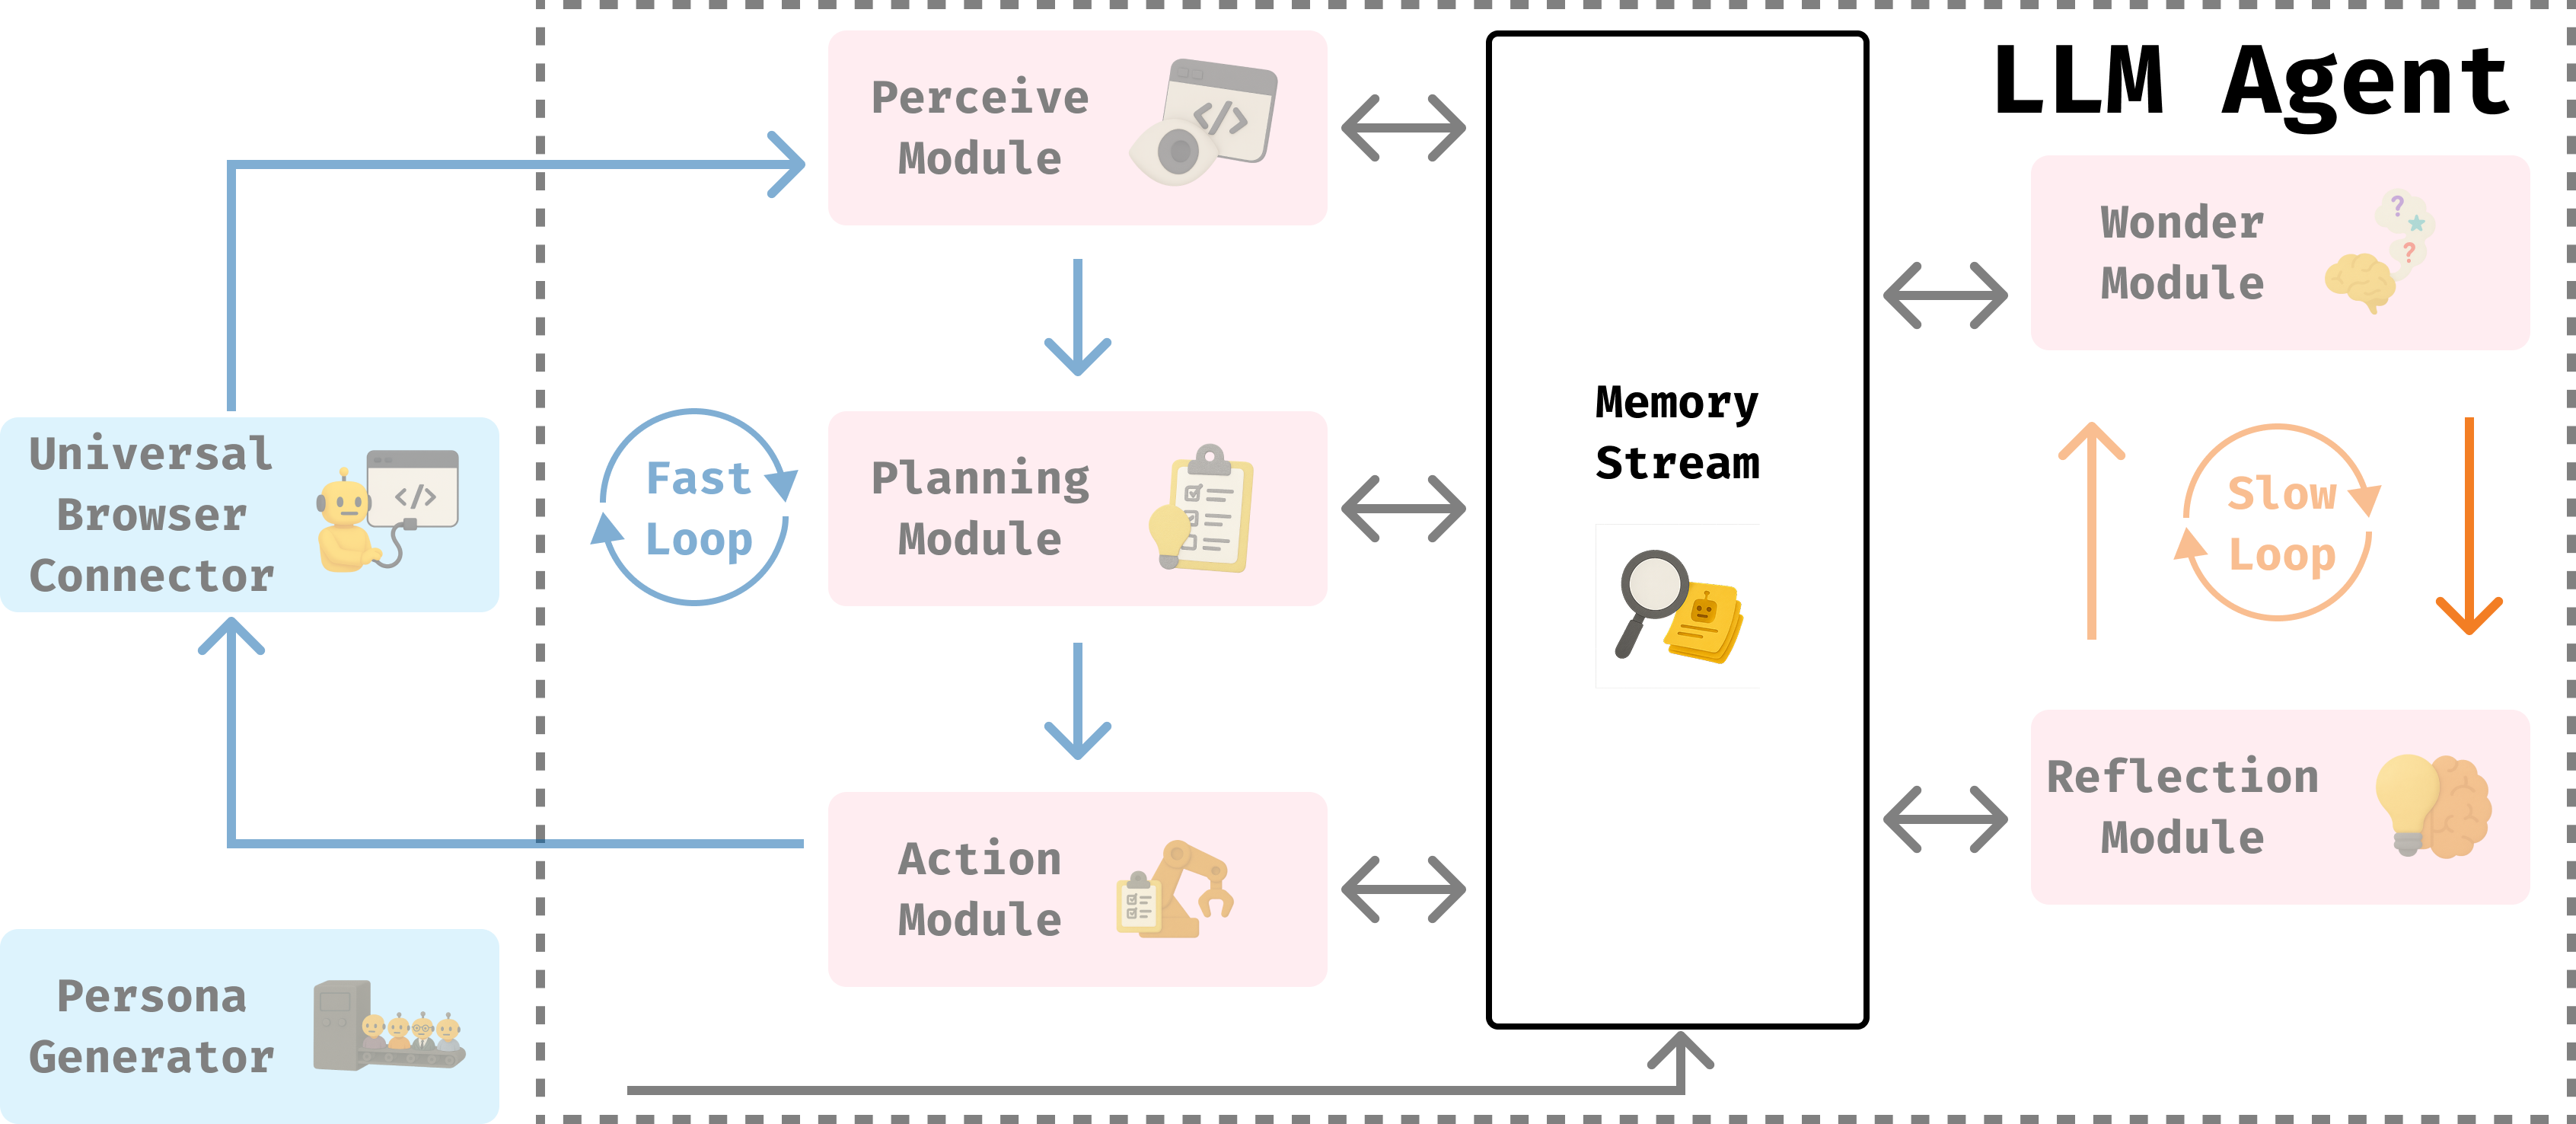
\includegraphics[width=\linewidth]{figures/structure-memory@2x.png}
  \end{figure}
\end{frame}

\begin{frame}{Agent Architecture - Collected Data}
  \begin{figure}[htp]
    \centering
    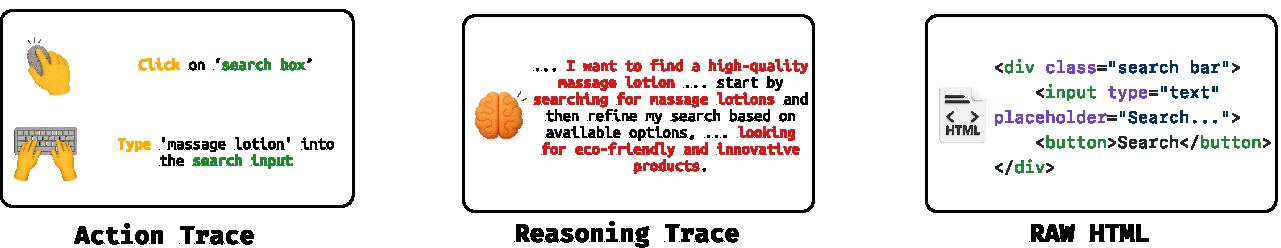
\includegraphics[width=\linewidth]{figures/data_collected.pdf}
  \end{figure}
\end{frame}

% \begin{frame}{Agent Architecture: Two-Loop + Memory}
  
%   \begin{outline}
%     \1 To allow both in-depth reasoning and real-time simulation:
%     \2 Fast Loop: rapid response to the outside environment
%     \2 Slow Loop: in-depth reasoning and thinking
%     \1 Asynchronous; interact through Memory Stream
%     \1 Each module retrieves and generate memories
%     \pause
%     \1 Data collected from our LLM Agent:
%       \2 Action Trace: what the agent did
    
%       \2 Final Session Outcome: final action in the action trace. Completing the task / terminating the session
    
%       \2 Reasoning Trace: agents' internal memory entries for supporting qualitative analysis
%   \end{outline}
% \end{frame}

\begin{frame}{Result Viewer Interface}
  \begin{figure}[htp]
    \centering
    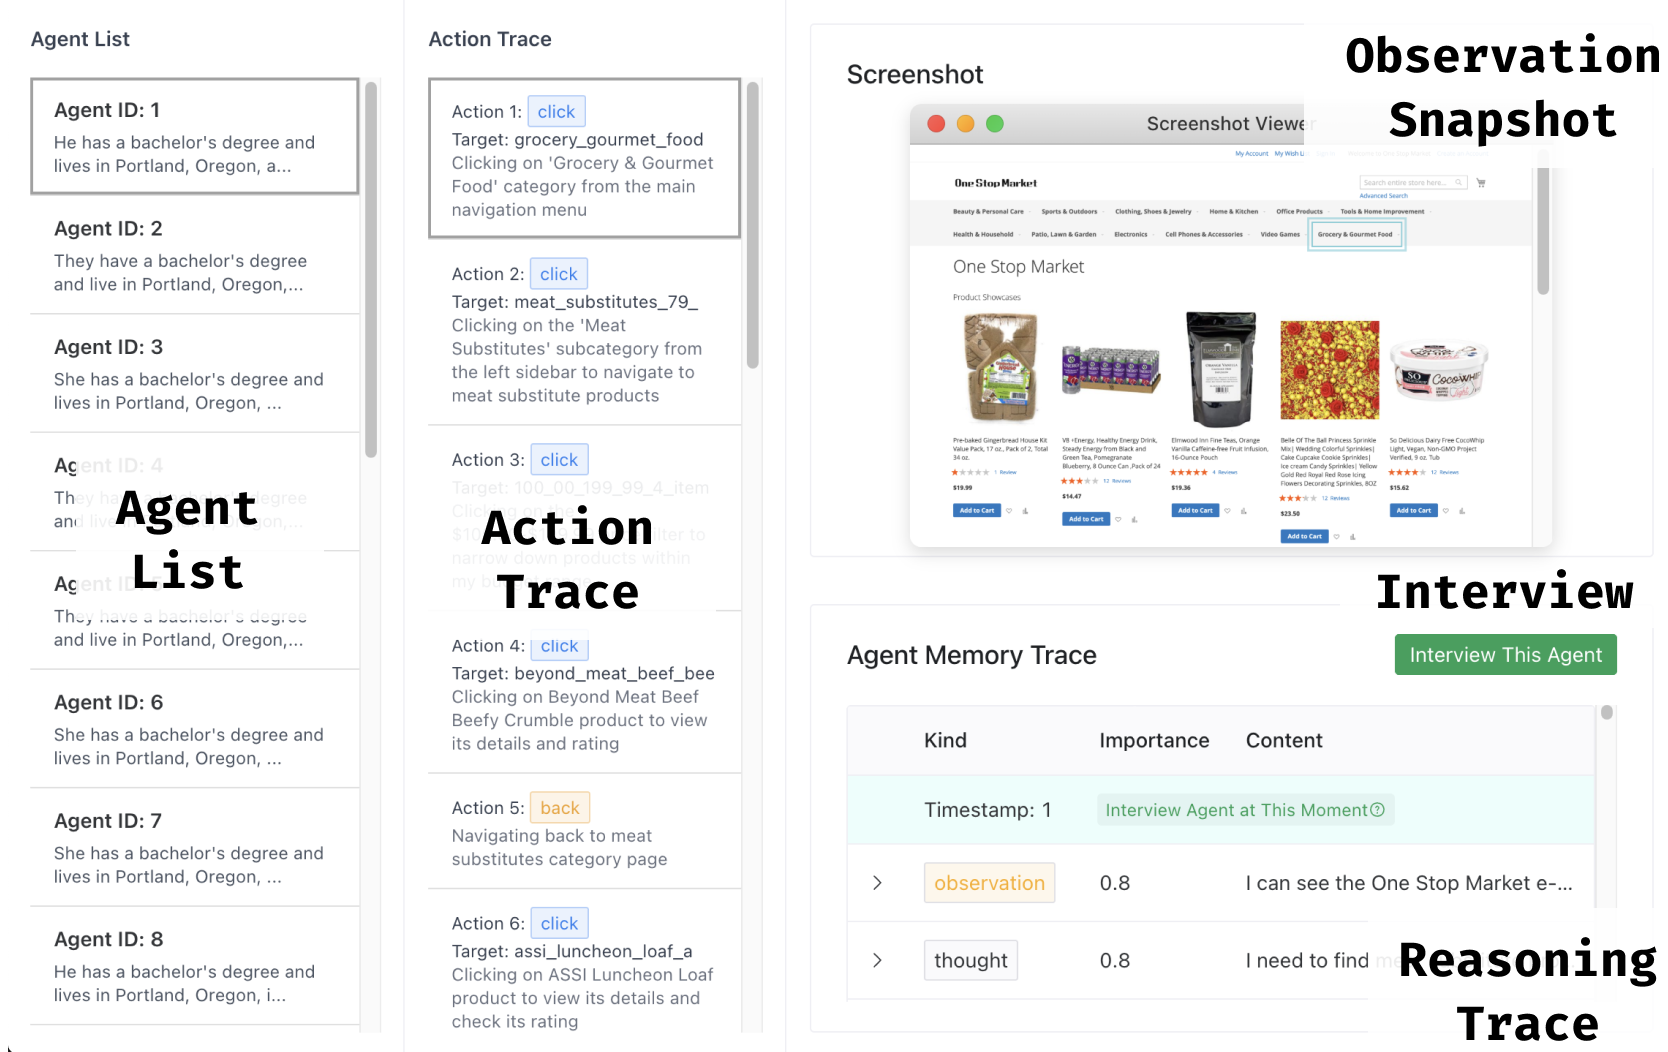
\includegraphics[width=.7\linewidth]{figures/uxagent/result-viewer-detail.png}
    \caption{Result Viewer Interface}
  \end{figure}
\end{frame}

\begin{frame}{Universal Browser Connector}
  \begin{figure}[htp]
    \centering
    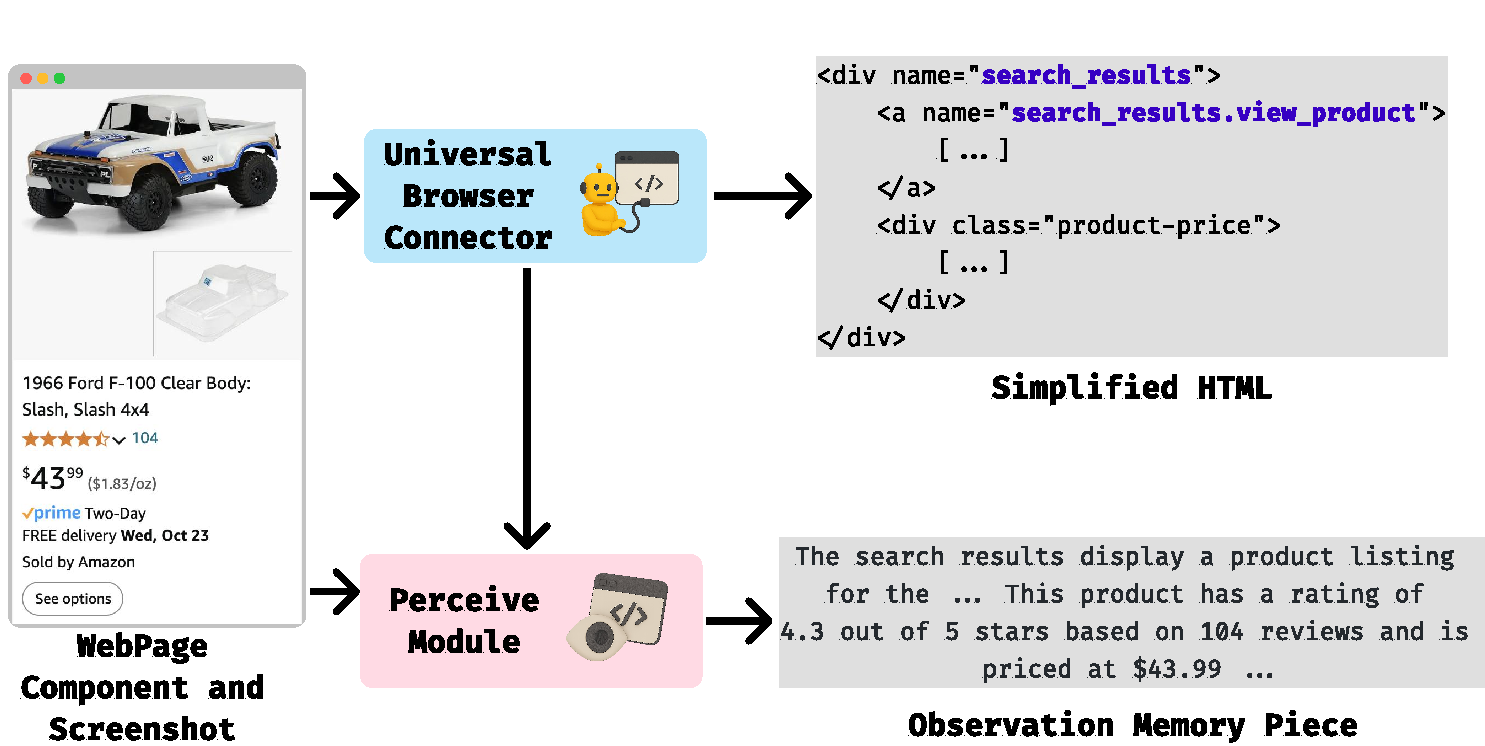
\includegraphics[width=.8\linewidth]{figures/uxagent/perception-demo.pdf}
    \caption{Universal Browser Connector}
  \end{figure}
\end{frame}

\begin{frame}[standout]
  UXAgent Evaluation: can simulated agents help UX researchers?
\end{frame}

\begin{frame}{User Study Setup}
  \begin{center}
    \small 16 UX researchers \quad$\cdot$\quad 20 simulated sessions \quad$\cdot$\quad \textasciitilde30 min / session
  \end{center}
  \vfill
  \begin{figure}
    \centering
    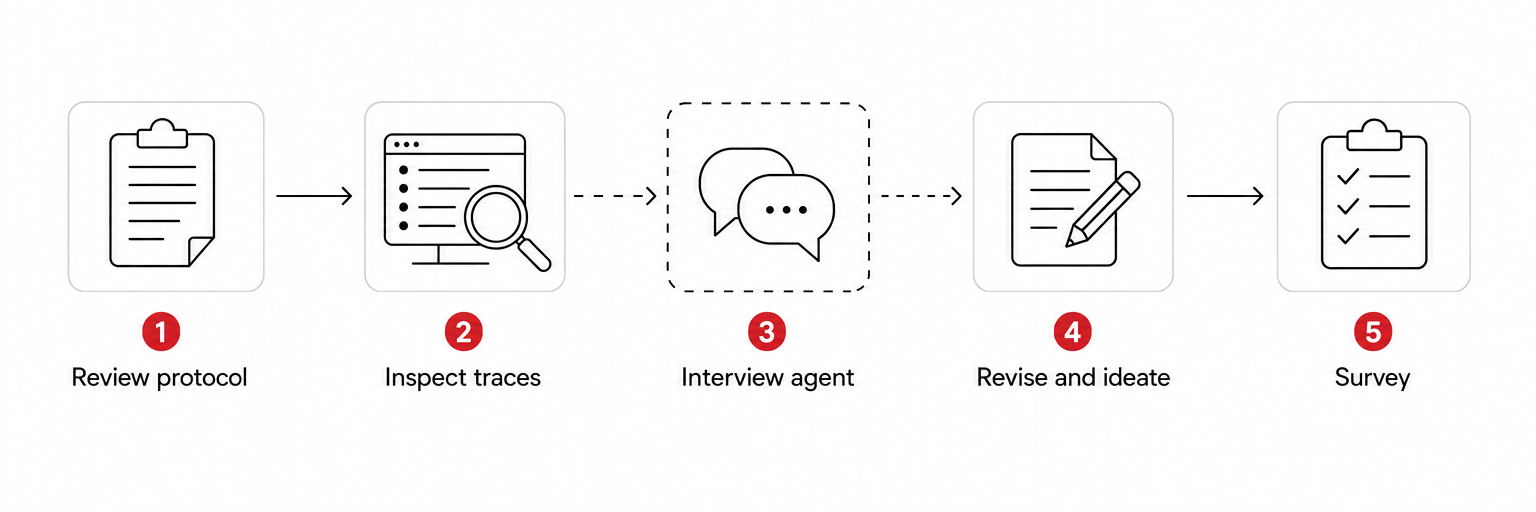
\includegraphics[width=\linewidth]{figures/uxagent/study_flow.png}
  \end{figure}
  \vfill
  \begin{center}
    \small Task: buy a meat substitute (top-rated, \$100--200), stop at checkout
  \end{center}
\end{frame}

\begin{frame}{Post-Study Ratings (Likert -2 to 2)}
  \centering
  \resizebox{.9\linewidth}{!}{%
  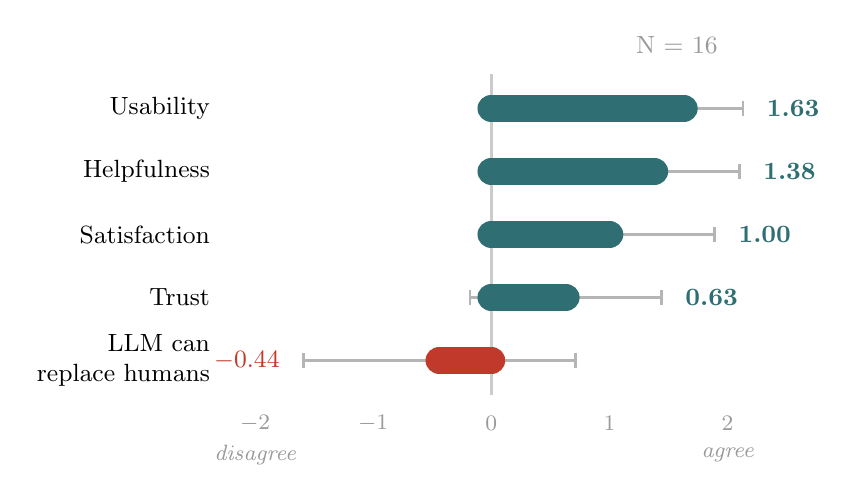
\begin{tikzpicture}[x=1.5cm,y=0.8cm]
    \draw[zeroln,line width=1.2pt] (0,-0.55) -- (0,4.55);
    \likertbar{4}{1.63}{0.50}{barpos}{1.63}
    \likertbar{3}{1.38}{0.72}{barpos}{1.38}
    \likertbar{2}{1.00}{0.89}{barpos}{1.00}
    \likertbar{1}{0.63}{0.81}{barpos}{0.63}
    \draw[whisk,line width=1pt] ({-0.44-1.15},0) -- ({-0.44+1.15},0);
    \draw[whisk,line width=1pt] ({-0.44-1.15},-0.12) -- ({-0.44-1.15},0.12);
    \draw[whisk,line width=1pt] ({-0.44+1.15},-0.12) -- ({-0.44+1.15},0.12);
    \draw[barneg,line width=10pt,line cap=round] (0,0) -- (-0.44,0);
    \node[barneg,anchor=east,font=\small\bfseries] at ({-0.44-1.15-0.12},0) {$-0.44$};
    \node[anchor=east,font=\small] at (-2.30,4) {Usability};
    \node[anchor=east,font=\small] at (-2.30,3) {Helpfulness};
    \node[anchor=east,font=\small] at (-2.30,2) {Satisfaction};
    \node[anchor=east,font=\small] at (-2.30,1) {Trust};
    \node[anchor=east,font=\small,align=right] at (-2.30,0) {LLM can\\replace humans};
    \node[tickgray,font=\footnotesize] at (-2,-1.0) {$-2$};
    \node[tickgray,font=\footnotesize] at (-1,-1.0) {$-1$};
    \node[tickgray,font=\footnotesize] at (0,-1.0) {0};
    \node[tickgray,font=\footnotesize] at (1,-1.0) {1};
    \node[tickgray,font=\footnotesize] at (2,-1.0) {2};
    \node[tickgray,font=\footnotesize\itshape] at (-2,-1.5) {disagree};
    \node[tickgray,font=\footnotesize\itshape] at (2,-1.5) {agree};
    \node[tickgray,font=\small,anchor=east] at (2,5.0) {N = 16};
  \end{tikzpicture}}
  \centering\small Researchers find UXAgent usable and helpful --- but reject it as a \emph{replacement} for humans.
\end{frame}

\begin{frame}{Protocol Iteration Outcomes}
  \begin{columns}[c]
    \begin{column}{0.36\linewidth}
      \centering
      {\fontsize{46}{50}\selectfont\textbf{14/16}}\\[4pt]
      {\small proposed further study-design\\ changes after using UXAgent}
    \end{column}
    \begin{column}{0.62\linewidth}
      \resizebox{\linewidth}{!}{%
      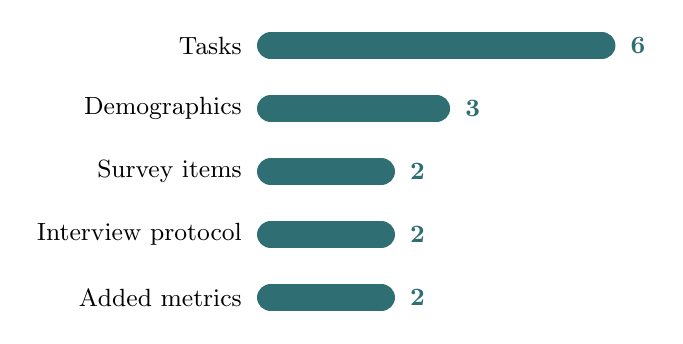
\begin{tikzpicture}[x=0.7cm,y=0.8cm]
        \draw[barpos,line width=10pt,line cap=round] (0,4) -- (6,4);
        \node[barpos,anchor=west,font=\small\bfseries] at (6.35,4) {6};
        \node[anchor=east,font=\small] at (-0.35,4) {Tasks};
        \draw[barpos,line width=10pt,line cap=round] (0,3) -- (3,3);
        \node[barpos,anchor=west,font=\small\bfseries] at (3.35,3) {3};
        \node[anchor=east,font=\small] at (-0.35,3) {Demographics};
        \draw[barpos,line width=10pt,line cap=round] (0,2) -- (2,2);
        \node[barpos,anchor=west,font=\small\bfseries] at (2.35,2) {2};
        \node[anchor=east,font=\small] at (-0.35,2) {Survey items};
        \draw[barpos,line width=10pt,line cap=round] (0,1) -- (2,1);
        \node[barpos,anchor=west,font=\small\bfseries] at (2.35,1) {2};
        \node[anchor=east,font=\small] at (-0.35,1) {Interview protocol};
        \draw[barpos,line width=10pt,line cap=round] (0,0) -- (2,0);
        \node[barpos,anchor=west,font=\small\bfseries] at (2.35,0) {2};
        \node[anchor=east,font=\small] at (-0.35,0) {Added metrics};
      \end{tikzpicture}}
    \end{column}
  \end{columns}
  
\end{frame}

\begin{frame}{Typical Iteration Cadence}
  \vfill
  \begin{figure}
    \centering
    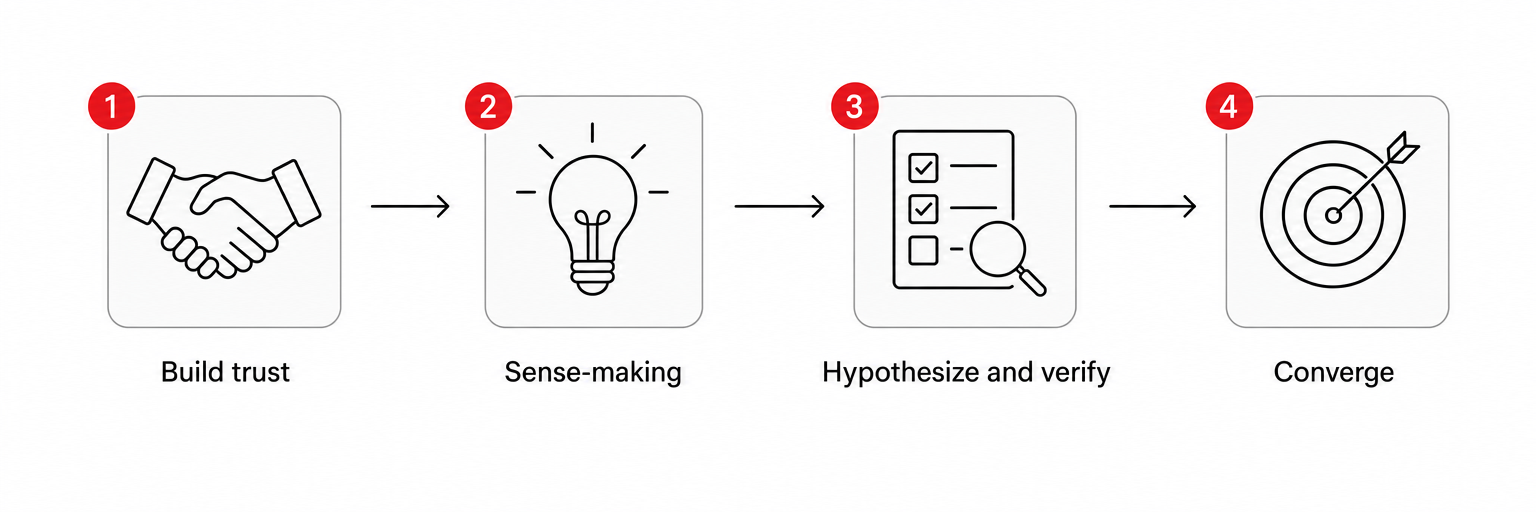
\includegraphics[width=\linewidth]{figures/uxagent/cadence_flow.png}
  \end{figure}
  \vfill
\end{frame}

\begin{frame}[c]{Trust comes from cross-modal alignment}
  \centering
  {\color{barpos}\fontsize{42}{42}\selectfont ``}\par
  \vspace{-0.2em}
  \begin{minipage}{0.82\linewidth}\centering
    {\LARGE\itshape I trust it pretty much because it's aligned with the reasoning.}
  \end{minipage}\par
  \vspace{0.5em}
  {\bfseries --- P3}\par
  \vspace{1.6em}
  {\small Researchers cross-check \textbf{reasoning $\leftrightarrow$ action $\leftrightarrow$ screenshot} before trusting the data.\quad Trust rated $M=0.62$ (SD~0.81).}
\end{frame}

\begin{frame}[c]{Is the behavior human-like? Mixed.}
  \begin{columns}[t]
    \begin{column}{0.46\linewidth}\centering
      {\color{barpos}\large\bfseries convincing}\par\vspace{0.5em}
      {\large\itshape ``The reasoning of the actions is very reasonable.''}\par
      \vspace{0.4em}{\bfseries --- P7}
    \end{column}
    \begin{column}{0.46\linewidth}\centering
      {\color{barneg}\large\bfseries not convincing}\par\vspace{0.5em}
      {\large\itshape ``I just do not think a real human participant will have actions like that.''}\par
      \vspace{0.4em}{\bfseries --- P6}
    \end{column}
  \end{columns}
  \vspace{1.8em}
  \centering
  {\small \emph{\dots but} ``users always surprise me'' (\textbf{P8}) --- real users are unpredictable too, so some surprising agent behavior may feel \emph{authentic} rather than less.}
\end{frame}

\begin{frame}[c]{Complement, not replace}
  \centering
  {\color{barneg}\fontsize{42}{42}\selectfont ``}\par
  \vspace{-0.2em}
  \begin{minipage}{0.82\linewidth}\centering
    {\LARGE\itshape I'm really afraid that researchers only rely on this and overtrust such data.}
  \end{minipage}\par
  \vspace{0.5em}
  {\bfseries --- P1}\par
  \vspace{1.6em}
  {\small Most disagreed that agents can \textbf{replace} humans ($M=-0.44$).
  
  Position: \textbf{augment} human studies --- best for early, low-cost iteration.}
\end{frame}

\section[Case Study 2: Simulating Large-Scale A/B Testing Study with LLM Agents]{Case Study 2: Simulating Large-Scale A/B Testing Study with LLM Agents}

% =====================================================================
%  Case Study 2 — Agent A/B : Simulating Large-Scale A/B Testing
%  Frames only. \input this right AFTER the existing
%    \section[Case Study 2: Simulating Large-Scale A/B Testing ...]{...}
%  line in user-simulator.tex.
%  Figures live in figures/agentab/ (paper figures + GPT motivation art).
% =====================================================================

% ---- Bridge from UXAgent: small scale -> can it scale? ----
\begin{frame}[standout]
  UXAgent: LLM agents simulate users at \emph{small scale} to help UX researchers.
  \vspace{10pt}
  \pause

  But real design decisions ship through \emph{large-scale A/B testing}.
  \vspace{6pt}

  Can simulated users \ul{scale up}?
\end{frame}

\begin{frame}[plain]
  \begin{figure}[htp]
    \centering
    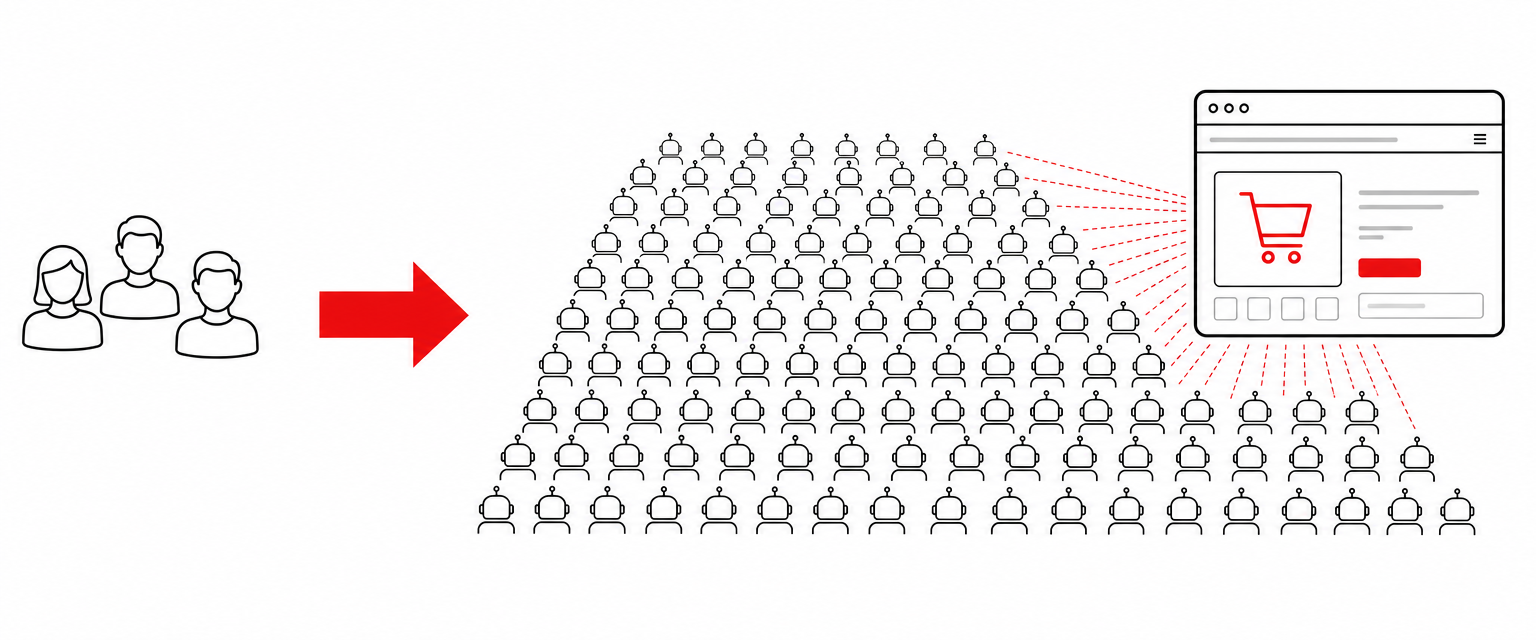
\includegraphics[width=\linewidth]{figures/agentab/scale_concept.png}
  \end{figure}
\end{frame}

% ---- What A/B testing is, and why it is heavy ----
\begin{frame}{Three Bottlenecks in A/B Testing}
  \begin{figure}[htp]
    \centering
    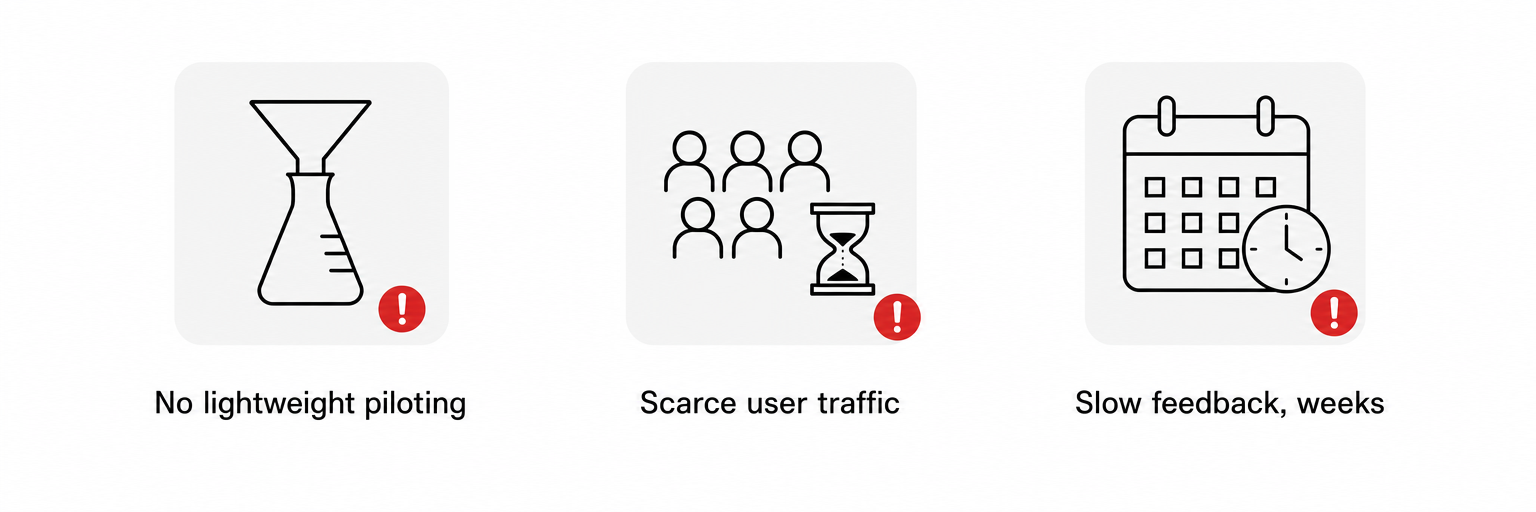
\includegraphics[width=\linewidth]{figures/agentab/bottlenecks.png}
  \end{figure}
  \centering\small From a formative study with 6 A/B-testing practitioners --- many promising ideas never get piloted before launch.
\end{frame}

% ---- The question ----
\begin{frame}[standout]
  Can we deploy \textbf{thousands} of persona-driven LLM agents on the \emph{live} website
  \vspace{6pt}

  --- to pilot an A/B test \ul{before} spending real user traffic?
\end{frame}

% ---- System overview ----
\begin{frame}{Our Solution: Agent A/B}
  \begin{figure}[htp]
    \centering
    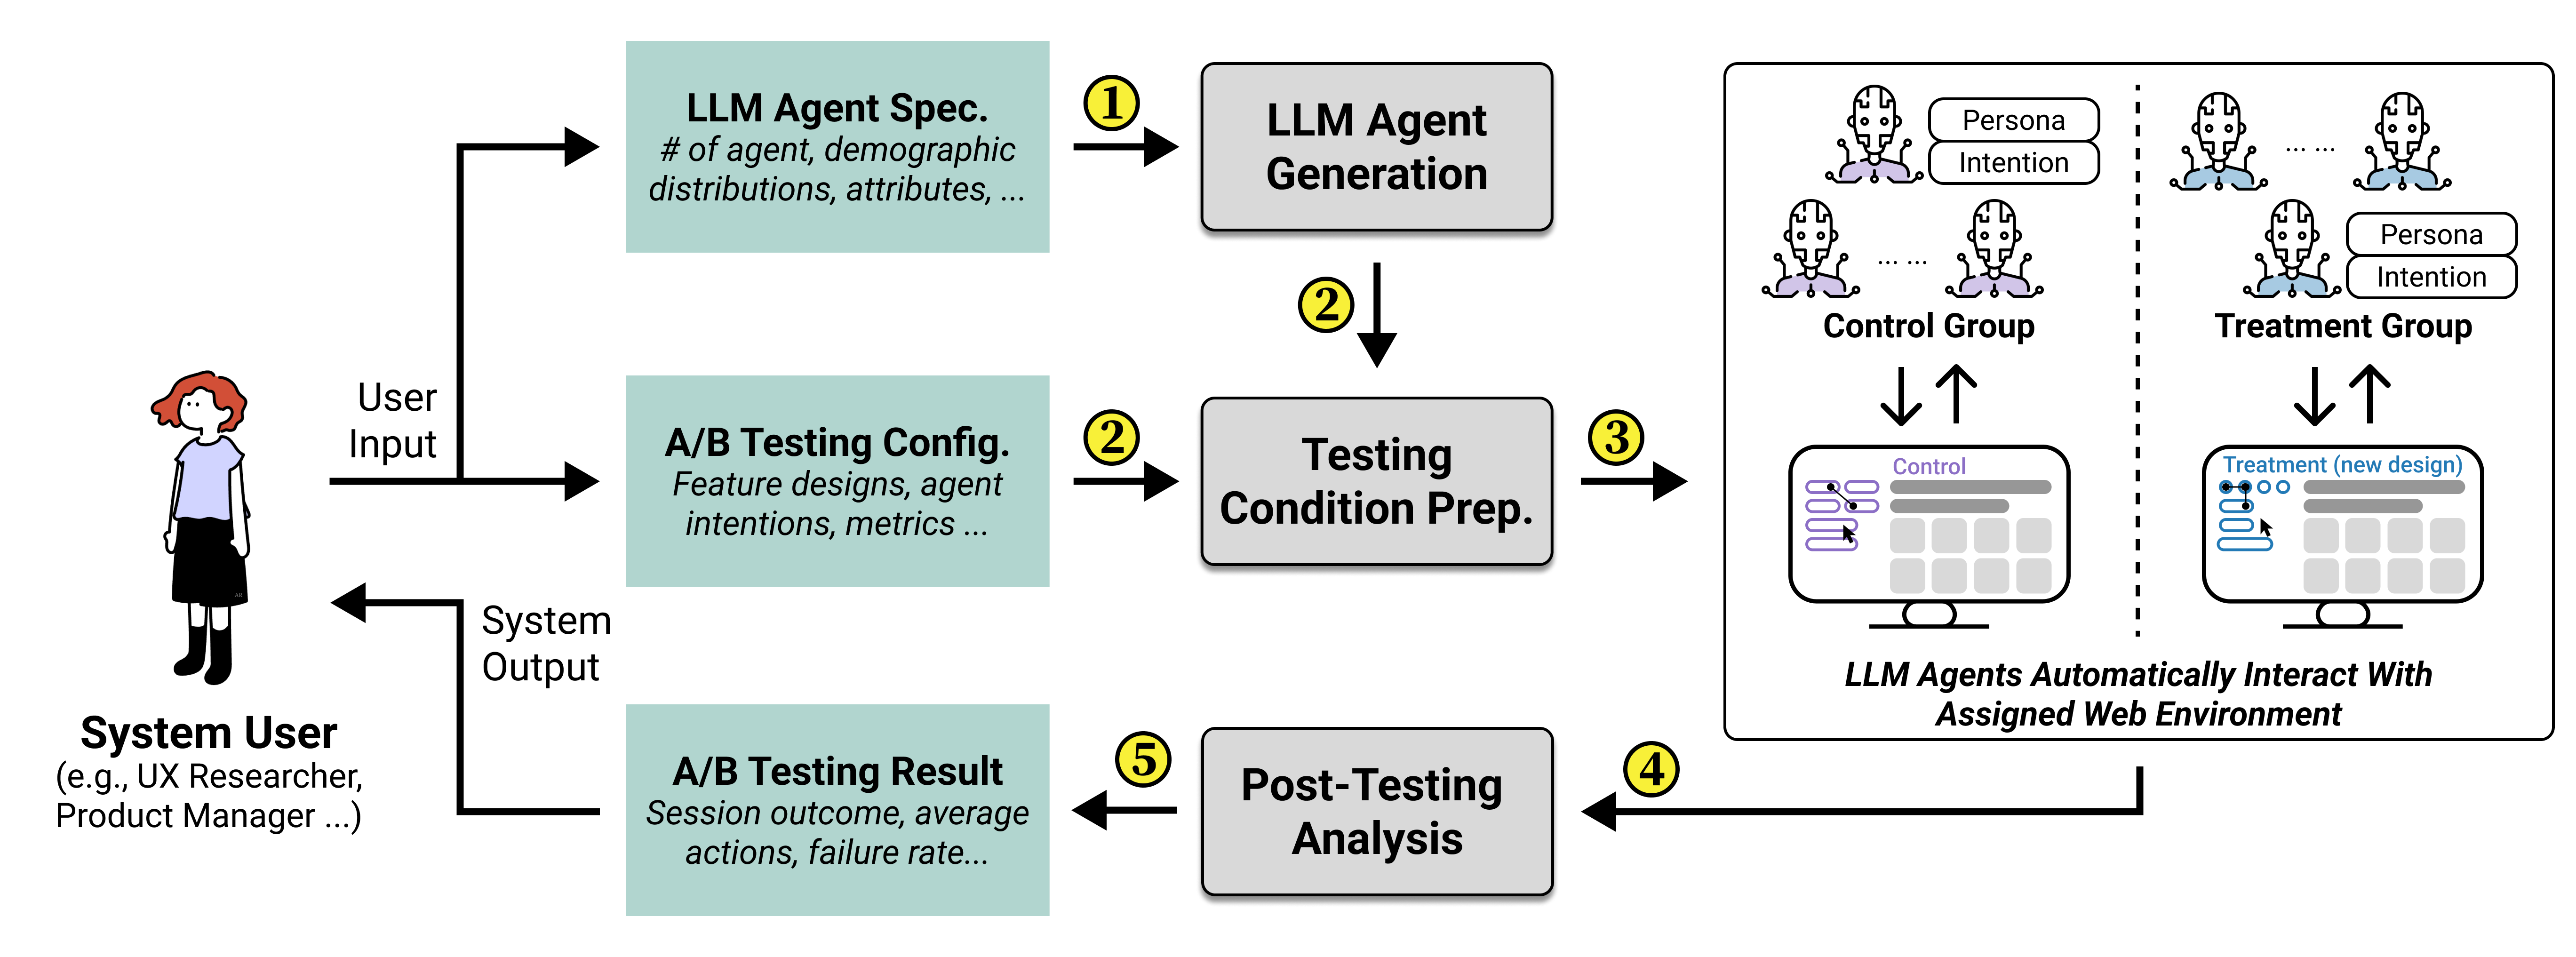
\includegraphics[width=\linewidth]{figures/agentab/abtest.png}
  \end{figure}
  \centering\small Plug-and-play with existing agent stacks (Claude computer-use, ReAct).
\end{frame}

% \begin{frame}{Inside One Agent}
%   \begin{figure}[htp]
%     \centering
%     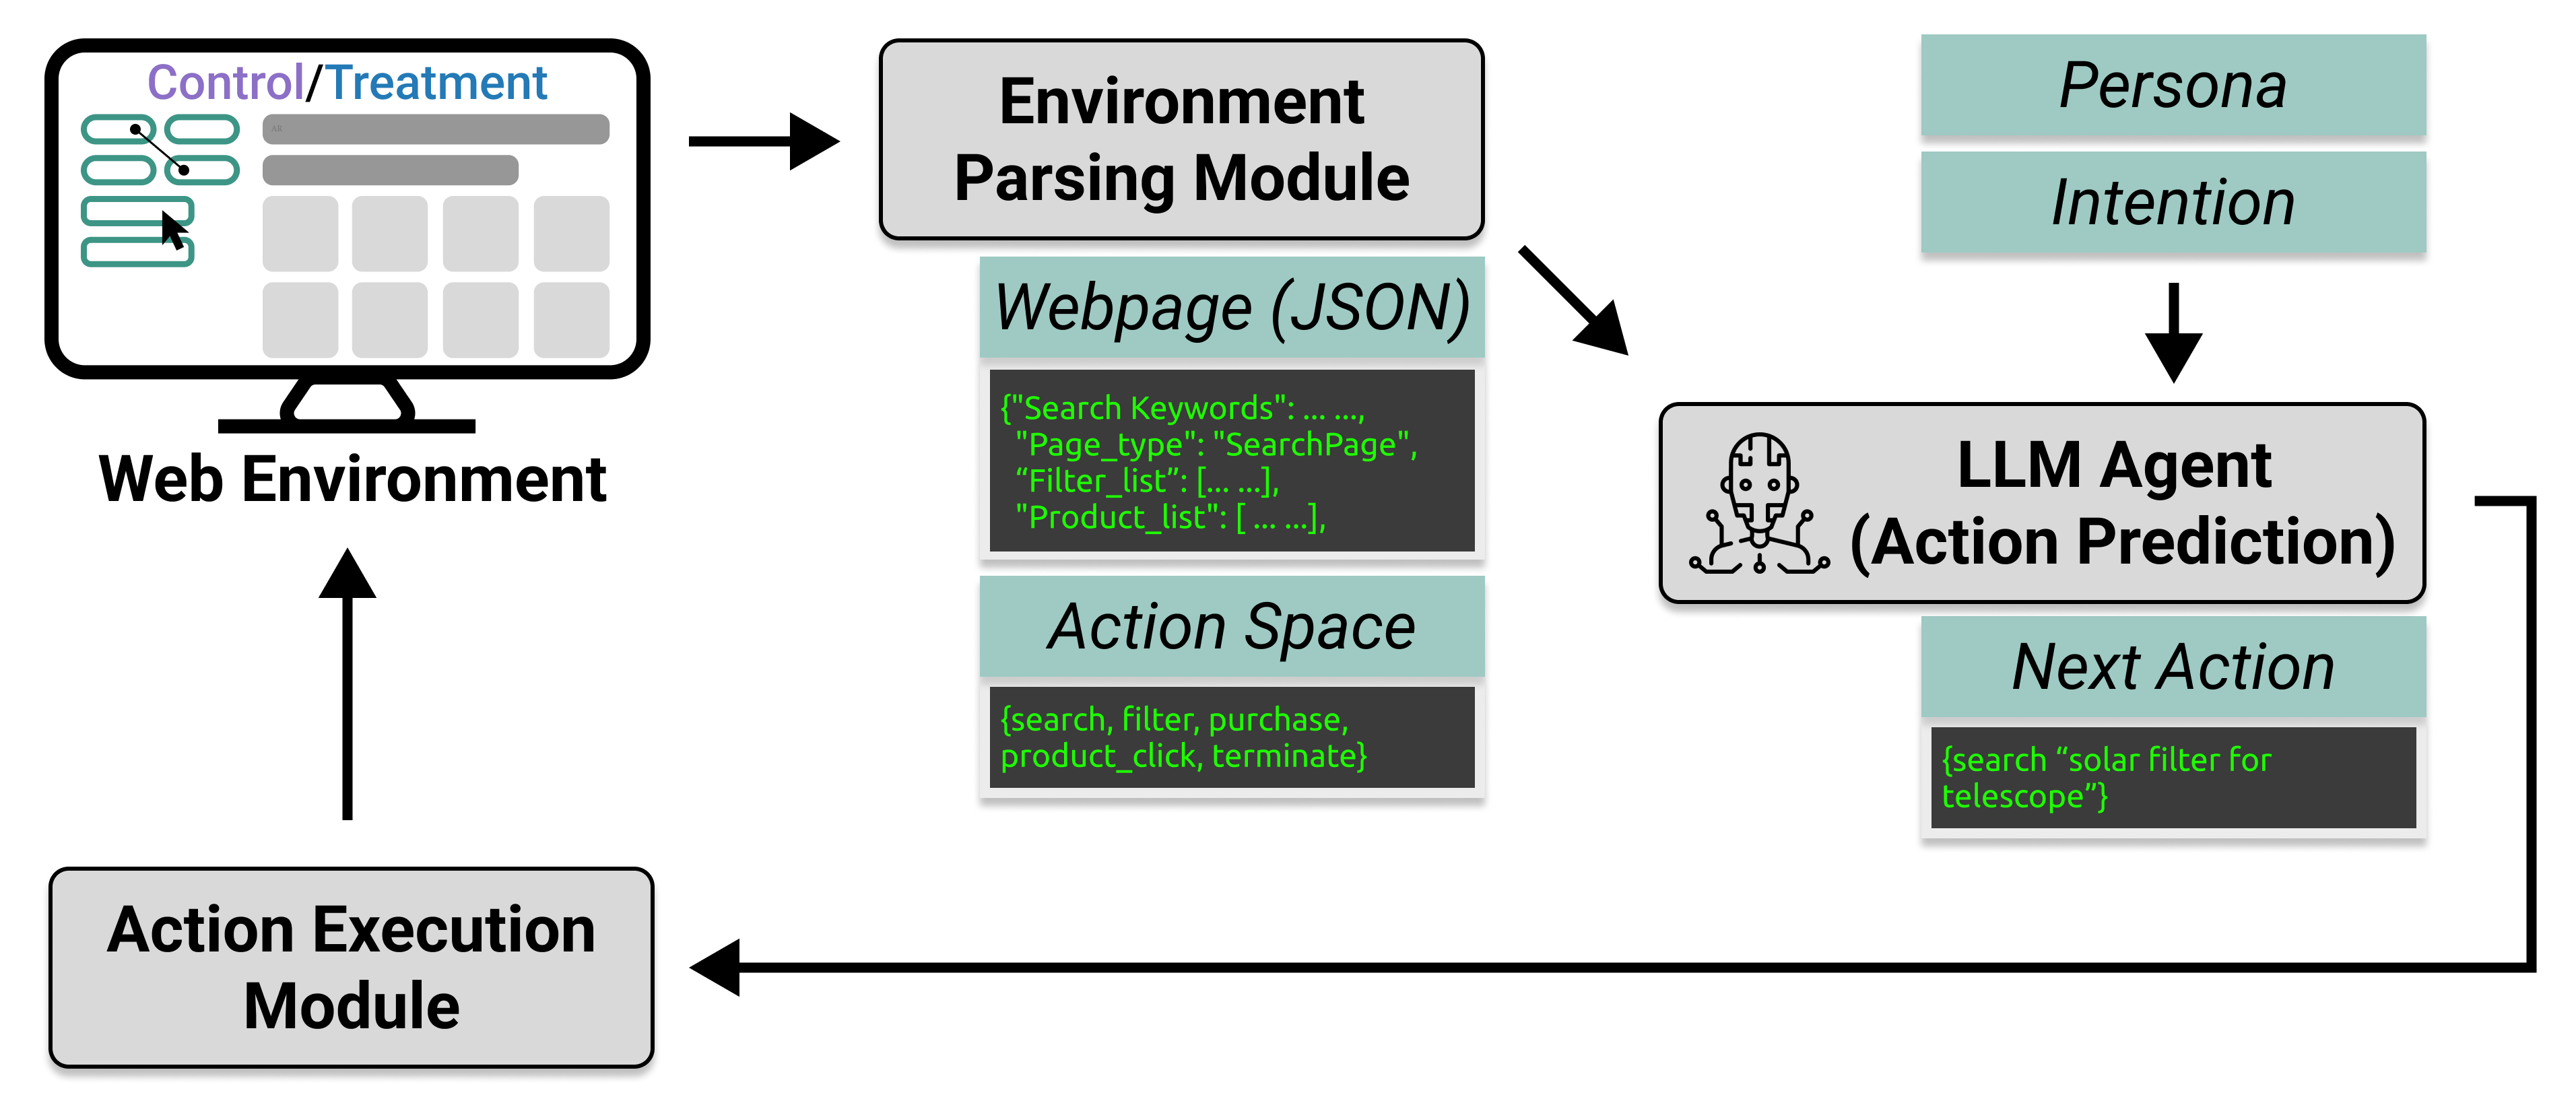
\includegraphics[width=.96\linewidth]{figures/agentab/system.png}
%   \end{figure}
% \end{frame}

% ---- Case study setup ----
\begin{frame}{Case Study: Amazon.com}
  \begin{figure}[htp]
    \centering
    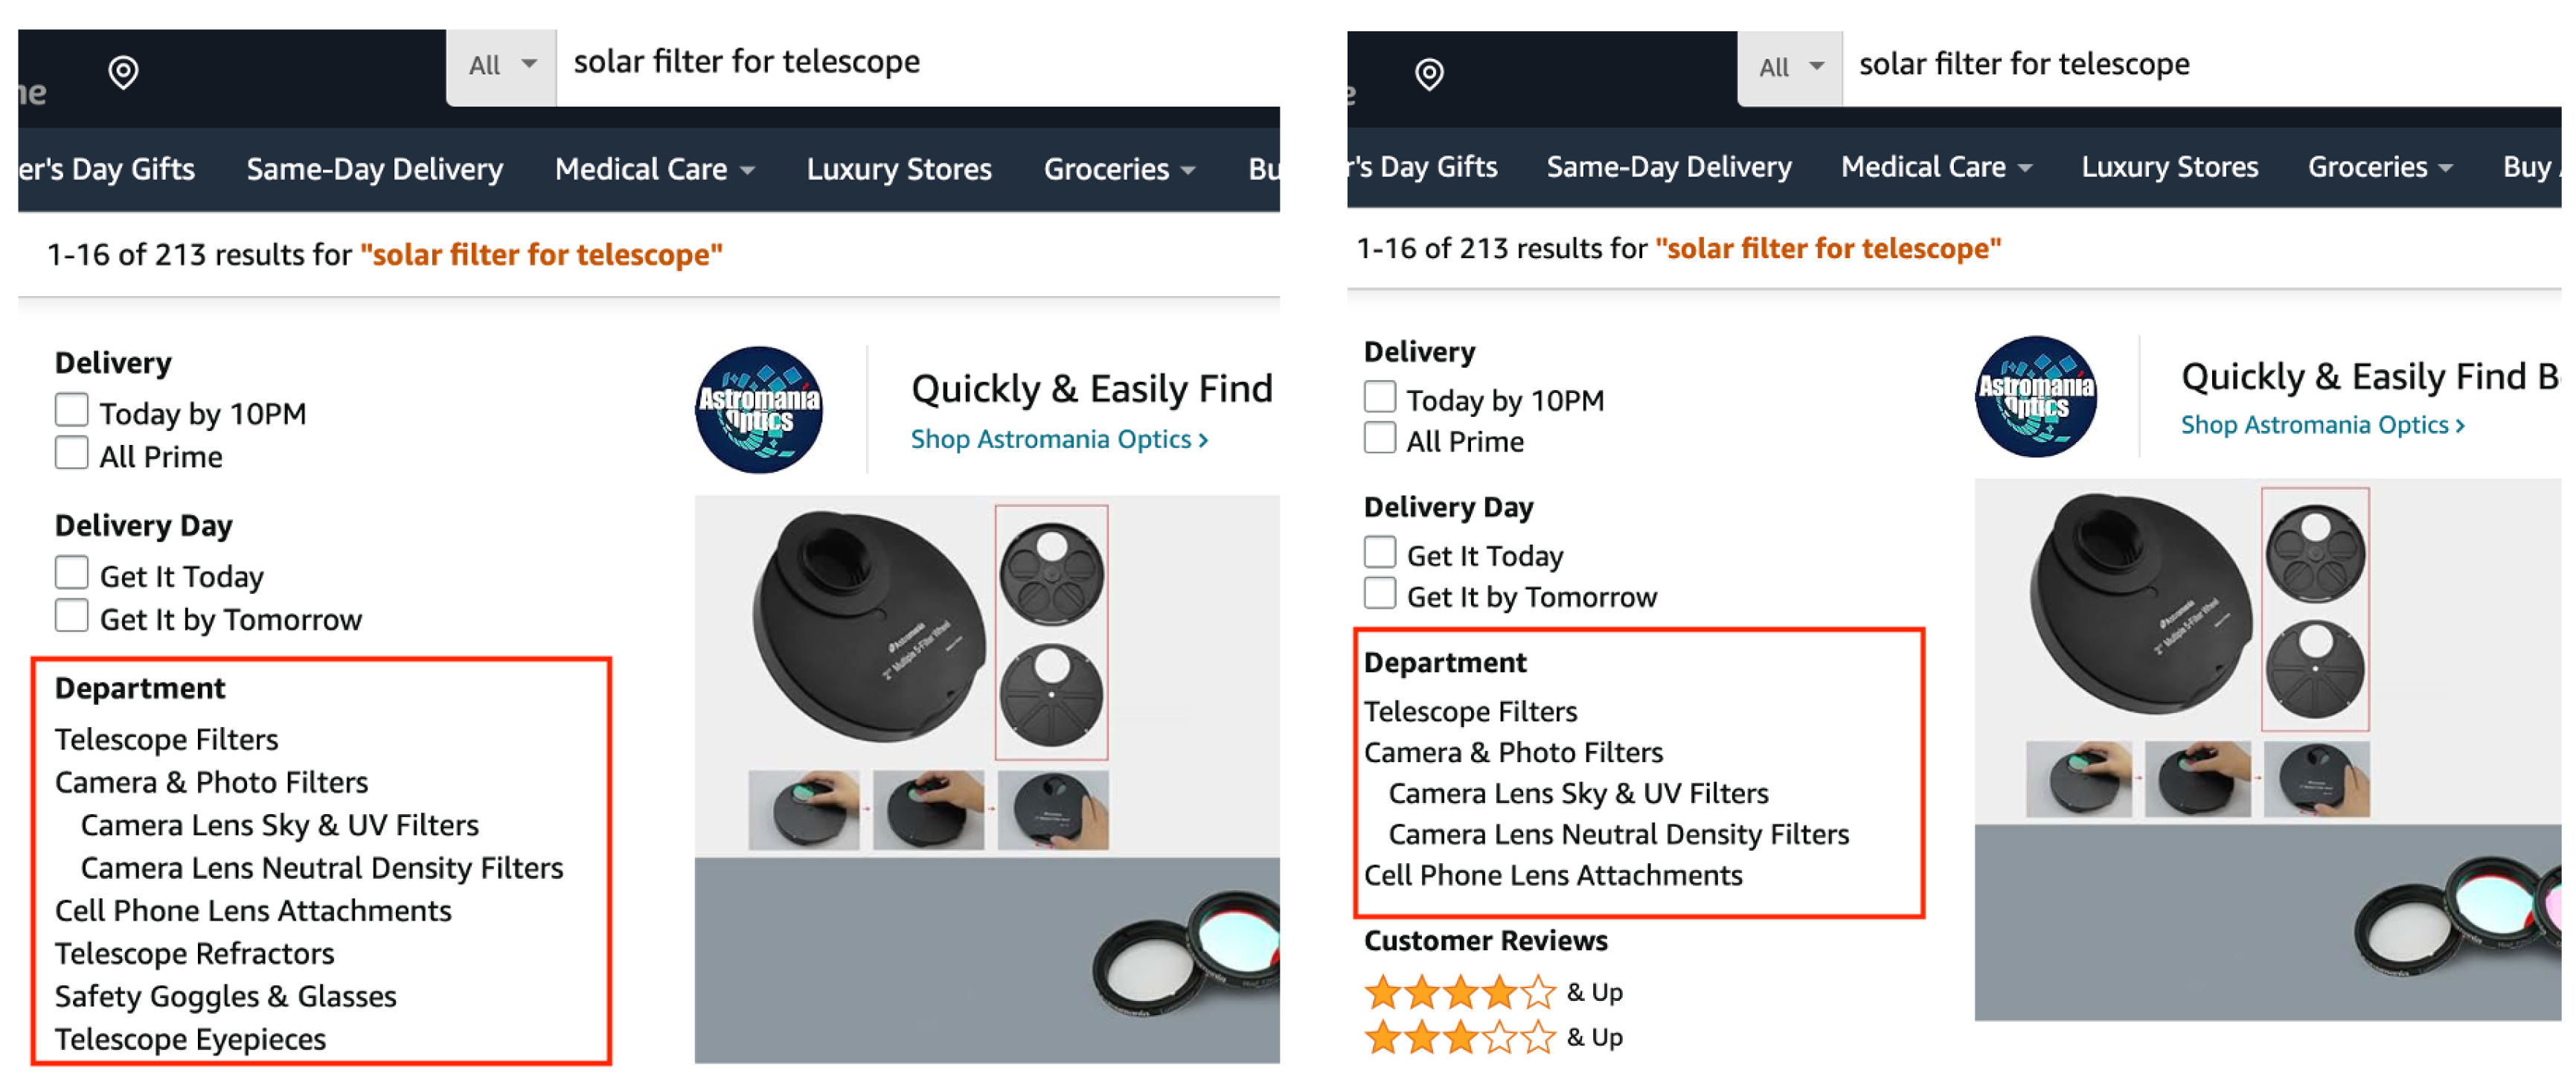
\includegraphics[width=.8\linewidth]{figures/agentab/filter_panel_design.png}
  \end{figure}
  \centering\small \textbf{Control}: full filter panel \quad vs.\quad \textbf{Treatment}: reduced panel (similarity ranking)\\
  \textbf{1,000} agents (500/condition) --- $\approx$10\% of a real A/B test.
\end{frame}

% ---- Results ----
\begin{frame}{Results: Reduced Filter $\rightarrow$ More Purchases}
  \begin{figure}[htp]
    \centering
    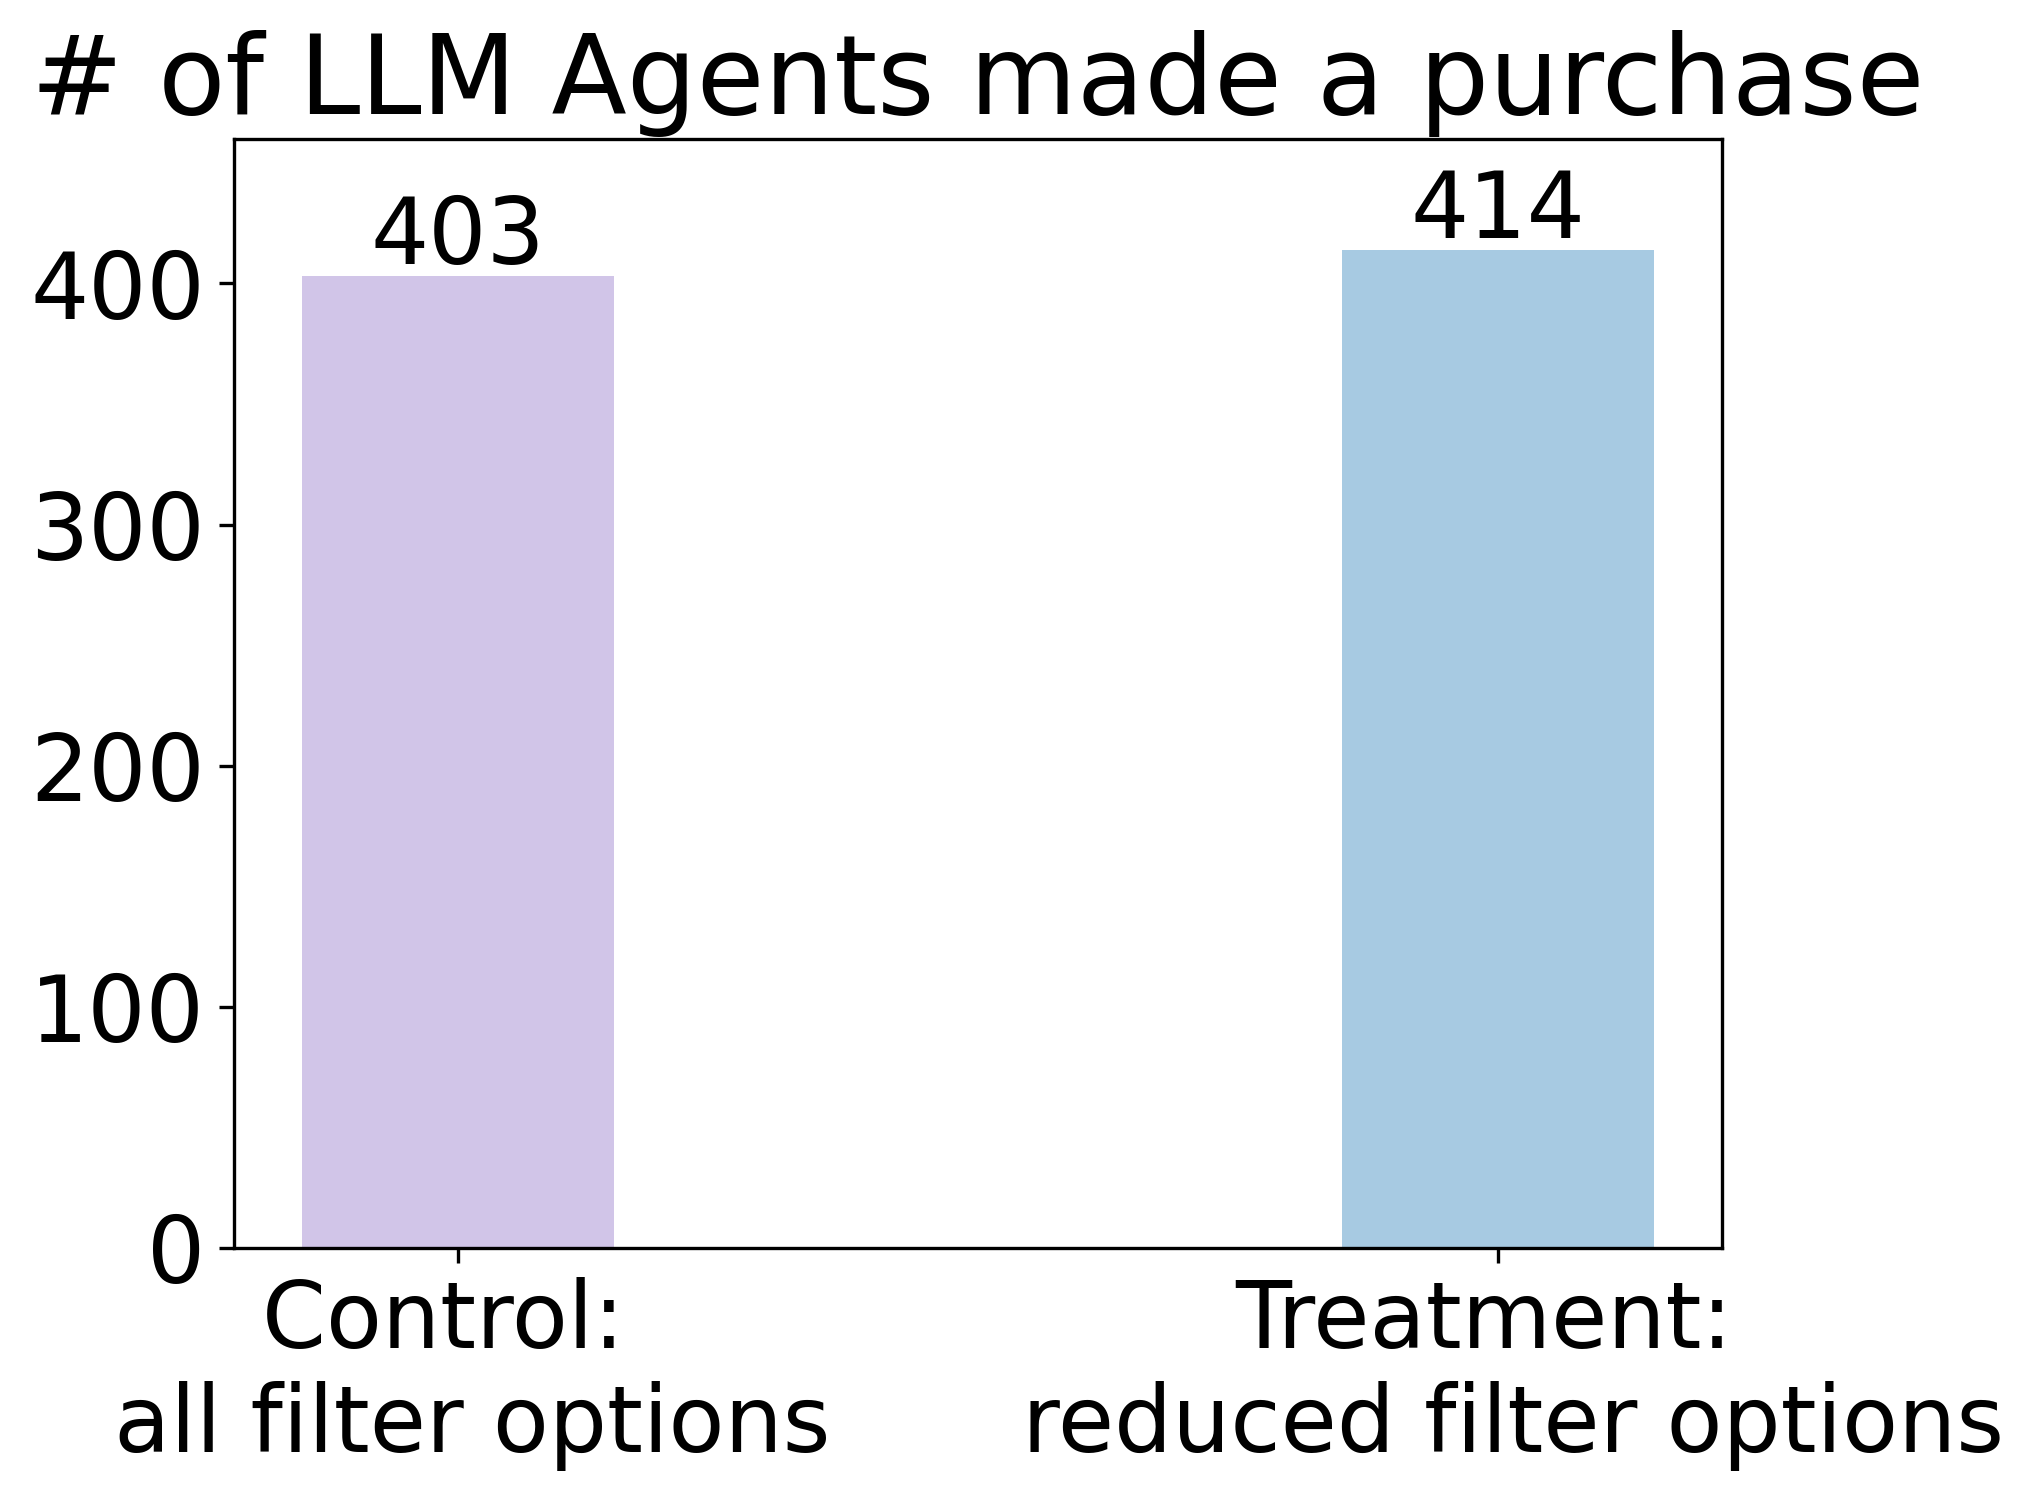
\includegraphics[width=.62\linewidth]{figures/agentab/bar.png}
  \end{figure}
  \centering\small \textbf{414 vs.\ 403} purchases --- a modest but statistically reliable increase.
\end{frame}

\begin{frame}{Subgroup Effects}
  \begin{columns}[c]
    \begin{column}{0.5\linewidth}
      \centering
      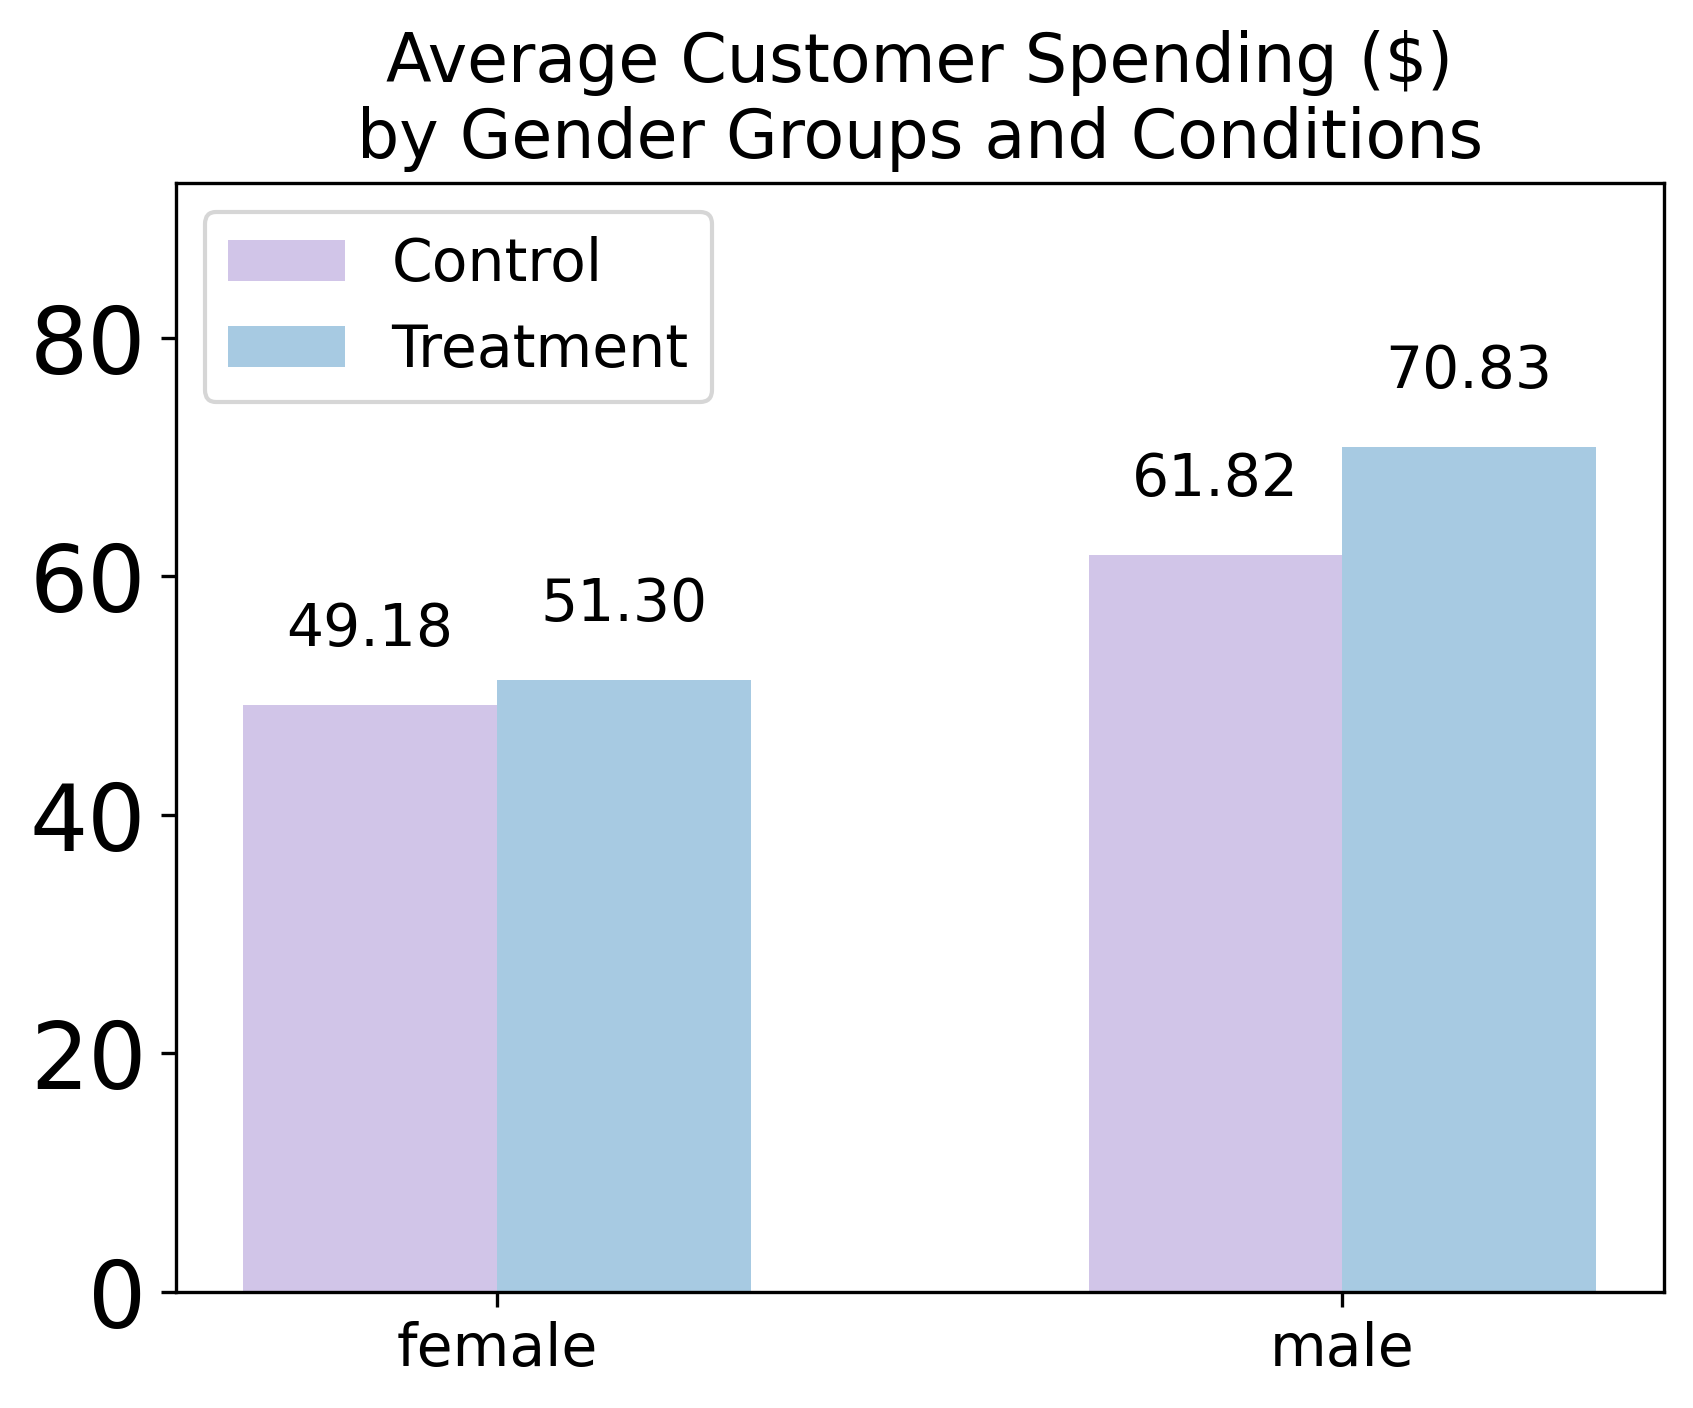
\includegraphics[width=\linewidth]{figures/agentab/control_treatment_gender_bar.png}
    \end{column}
    \begin{column}{0.5\linewidth}
      \centering
      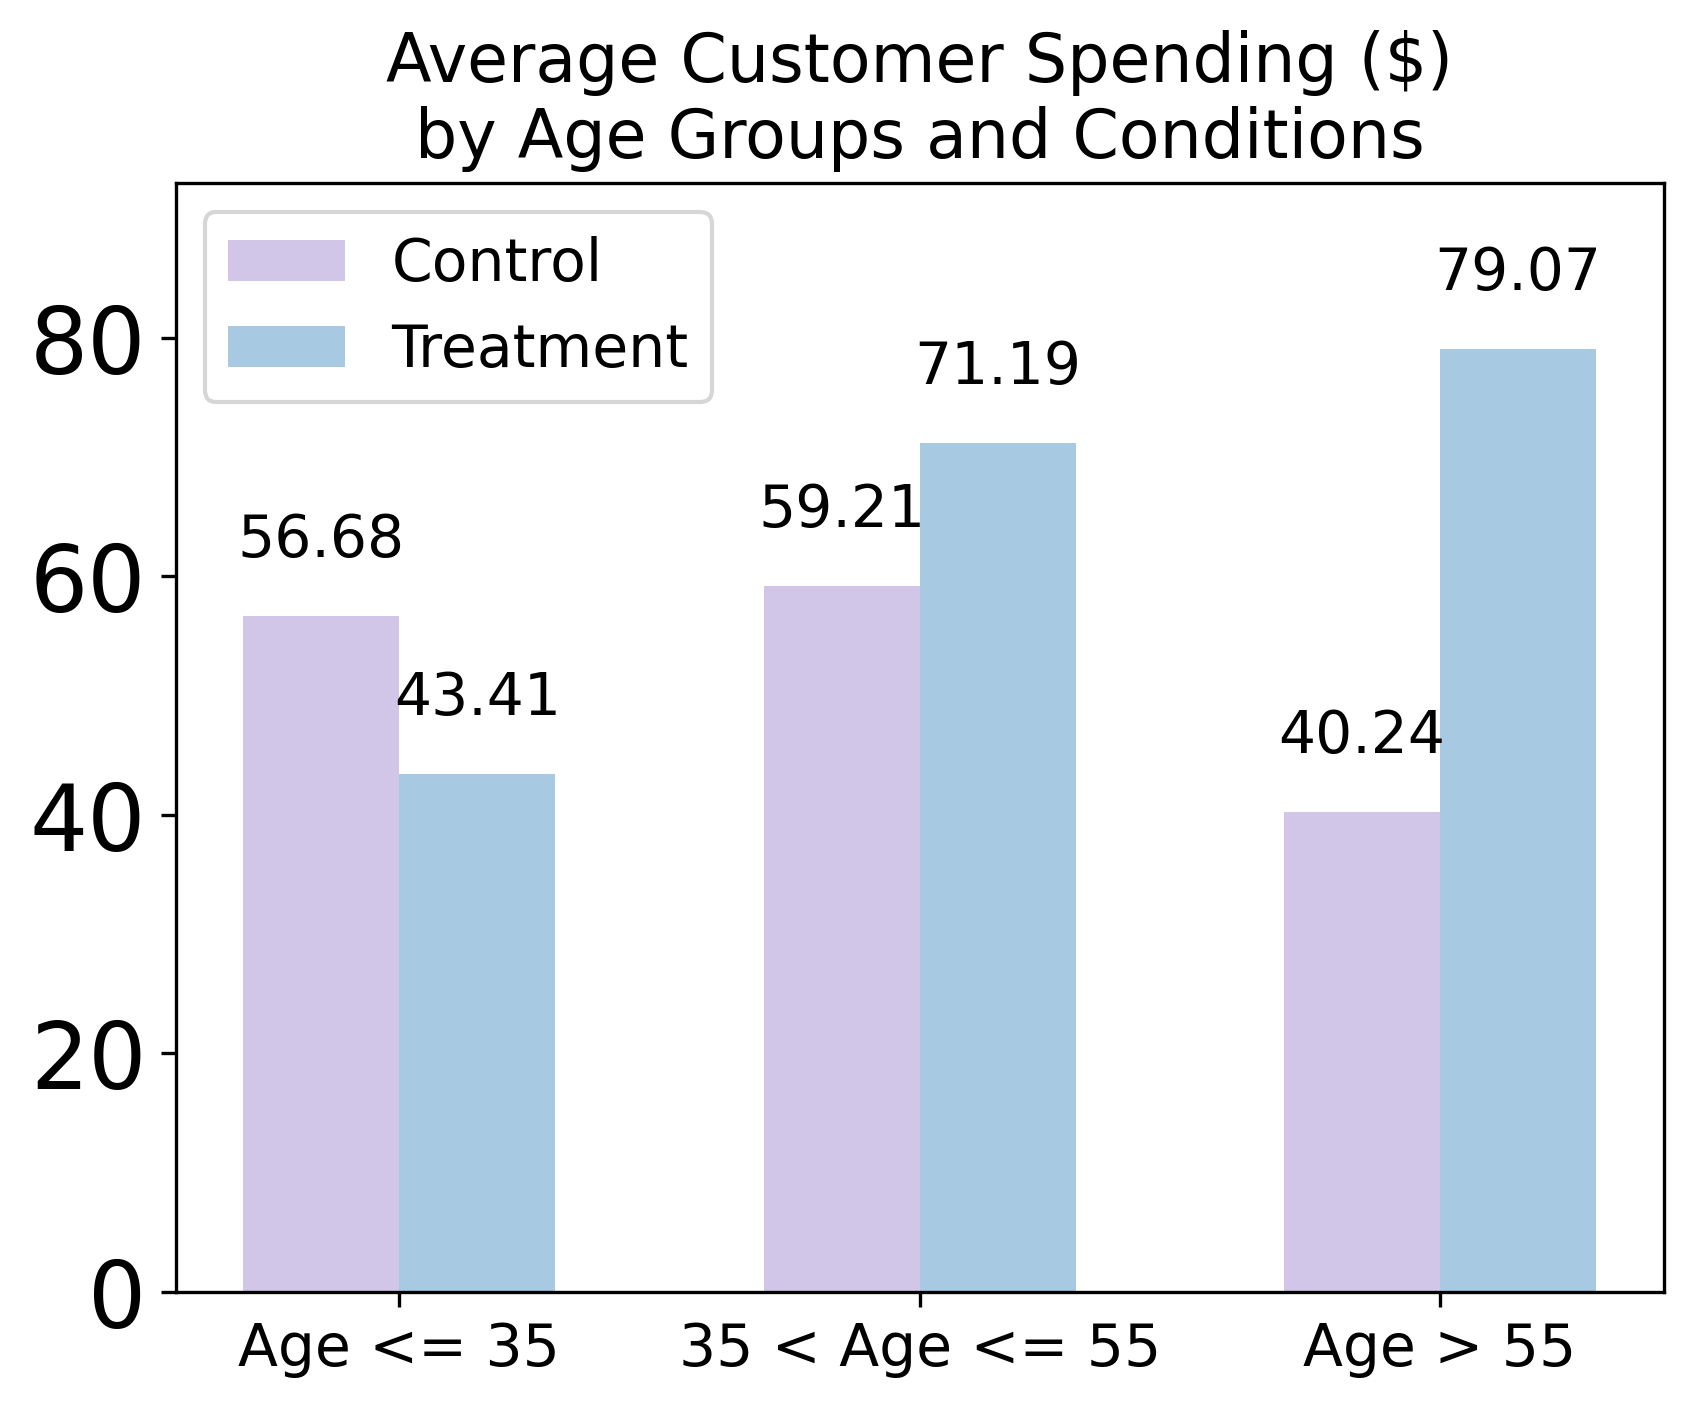
\includegraphics[width=\linewidth]{figures/agentab/control_treatment_age_bar.png}
    \end{column}
  \end{columns}
  \vspace{4pt}
  \centering\small Effects are stronger for \textbf{male} and \textbf{older} personas.
\end{frame}

% ---- Key validation ----
\begin{frame}[standout]
  Agent outcomes align \emph{directionally} with a parallel
  \textbf{large-scale human A/B experiment}.
\end{frame}

% ---- Handoff to Case Study 3 ----
\begin{frame}[standout]
  Simulated users can \ul{scale} --- \\ and point in the right direction.
  \vspace{10pt}
  \pause

  But ``directionally aligned'' $\neq$ ``accurate''.
  \vspace{4pt}

  \emph{How faithful are these agents, really?}
\end{frame}




\section[Case Study 3: Can LLM Agents Simulate Multi-Turn Human Behavior?]{Case Study 3: Use Real Online Customer Behavior Data to Evaluate and Improve}

% \begin{frame}{Motivation}
%   \begin{outline}
%     \1 Large Language Models (LLMs) have enabled the simulation of ``believable'' human behavior \cite{parkGenerativeAgentsInteractive2023}.
%     \1 Many application areas have emerged:
%       \2 Social Science Studies \cite{parkGenerativeAgentSimulations2024}
%       \2 UX Studies \cite{luUXAgentSystemSimulating2025}
%       \2 A/B Testing Studies \cite{wangAgentAAutomatedScalable2025}
%   \end{outline}
% \end{frame}

% \begin{frame}{Motivation}
%   \begin{outline}
%     \1 However, current systems are primarily optimized for and evaluated by their ``believability'':
%       \2 \textit{``how much people feel it is like a human''}
%     \1 rather than their ``accuracy'':
%       \2 \textit{``how much it acts like a human''}
%     \pause
%     \1 Some work evaluates the final outcomes of tasks (e.g., item purchases) \cite{yaoReActSynergizingReasoning2023}
%     \pause
%     \1 The fidelity of intermediate actions in the sequences are not quantitatively evaluated.
%   \end{outline}
% \end{frame}

% \begin{frame}[standout]
%   How can we better evaluate and improve LLM Agents' action accuracy in simulating human behavior?
% \end{frame}

% \begin{frame}[standout]
%   How can we better evaluate and improve LLM Agents' action accuracy in simulating human \textit{\ul{shopping}} behavior?
% \end{frame}

\subsection*{Task \& Method}

\begin{frame}{Task Definition}
  \begin{outline}
    \1 We focus on the \textbf{human behavior simulation task}
      \2 Generate the next user action based on the context and past actions.
      \2 Specifically, in the online shopping scenario.
  \end{outline}
  \begin{figure}
    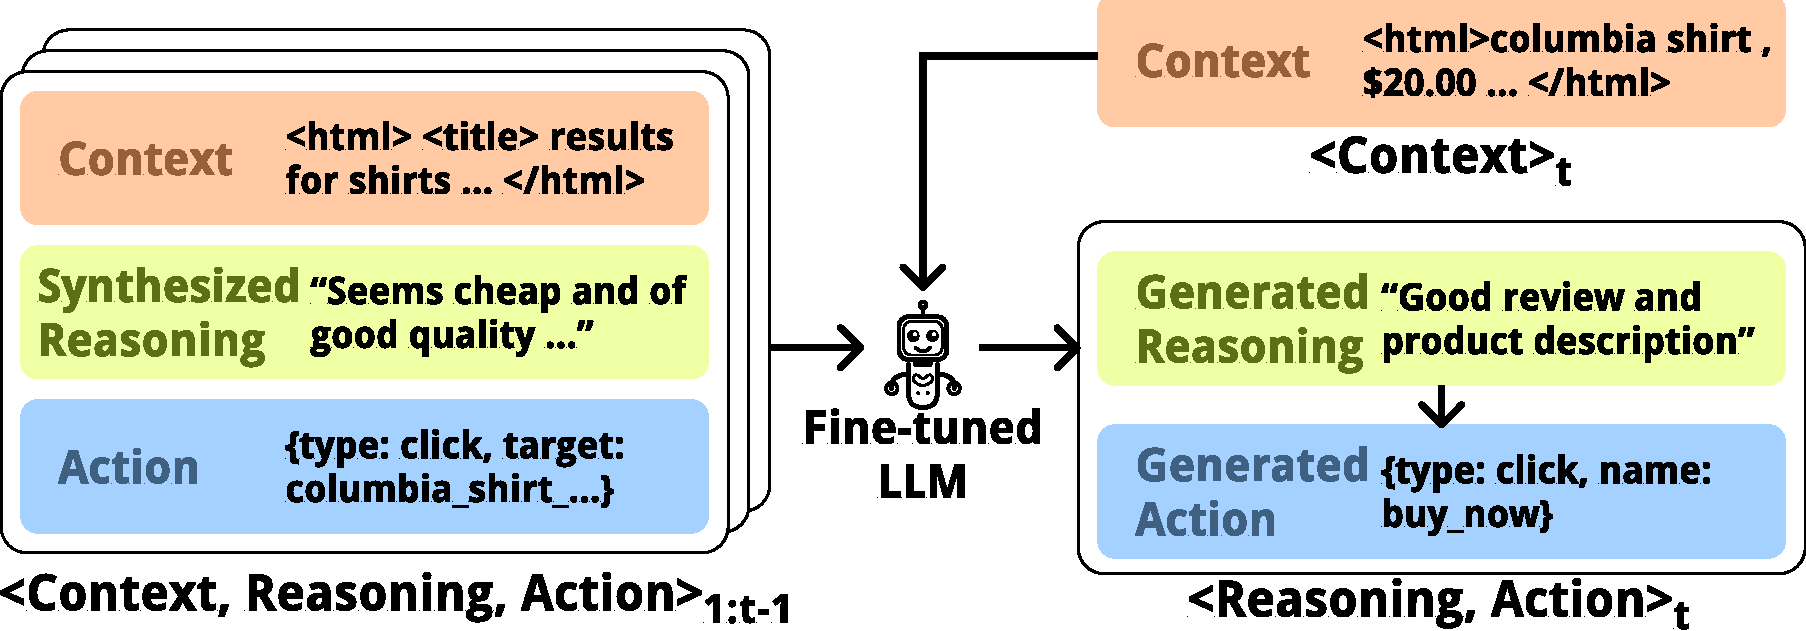
\includegraphics[width=\linewidth]{figures/finetuned_web_agent/teaser.pdf}
    \caption{Overview of the next action prediction task.}
  \end{figure}
\end{frame}

\begin{frame}{Dataset}
  \begin{outline}
    \1 Collected from a real-world online shopping platform.
    \1 31,865 sessions from 3,526 users
    \1 230,965 user actions
    \1 4,432 purchases, 27,433 terminations
  \end{outline}
\end{frame}

\begin{frame}{Context}
  \begin{columns}[c]
    \begin{column}{0.44\linewidth}
      \centering
      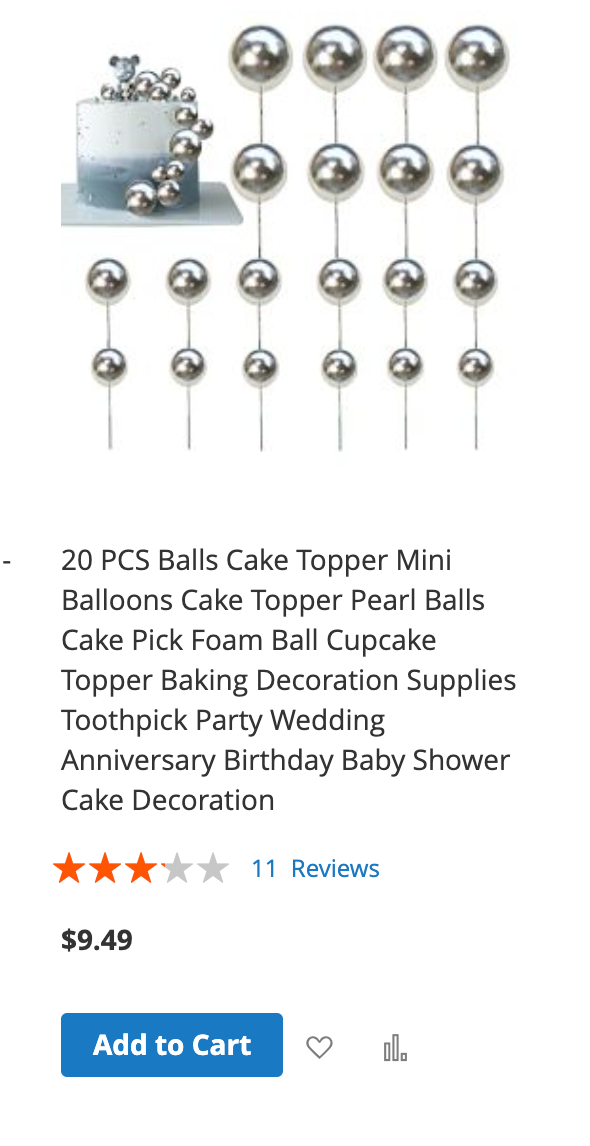
\includegraphics[height=.58\textheight]{figures/finetuned_web_agent/rawhtml.png}\\[2pt]
      {\small Rendered page}
    \end{column}
    \begin{column}{0.10\linewidth}
      \centering {\Large$\rightarrow$}
    \end{column}
    \begin{column}{0.44\linewidth}
      \centering
      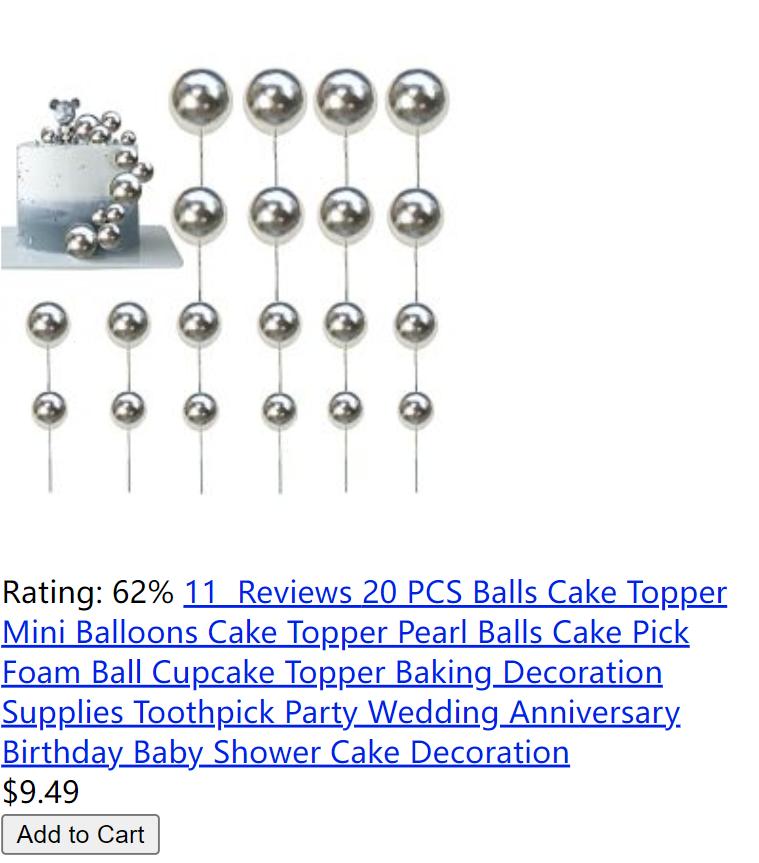
\includegraphics[height=.58\textheight]{figures/finetuned_web_agent/simplified-html.png}\\[2pt]
      {\small \textbf{Context}: simplified HTML}
    \end{column}
  \end{columns}
  \vspace{4pt}
  \centering {\small JS/CSS stripped, page structure kept; each interactable element gets a unique name (e.g.\ \code{product_form.add_to_cart}).}
\end{frame}
\begin{frame}{Action}
  \begin{outline}
    \1 \textbf{Action} is defined as the next raw browser action conducted by the user.
      \2 Generalizable to other domains beyond online shopping.
    \1 \code{click} (click on an element)
    \1 \code{type_and_submit} (type text and submit a form by hitting enter)
    \1 \code{terminate} (user ends the session by closing the browser window)
  \end{outline}
\end{frame}


\begin{frame}{Reasoning}
  \begin{outline}
    \1 \textbf{Reasoning} is defined as a natural language sentence that describes the reasoning behind an action.
      \2 \textit{``I want to find a comfortable piece of clothing, so I’m looking for options with high ratings.''}
    \1 Enhances the explainability of the model.
    \1 Not present in existing datasets.
    \1 Synthesize with teacher LLM
  \end{outline}
  
\end{frame}

% \begin{frame}{Rationale Synthesis}

%   \begin{outline}
%     \1 Reasoning traces are crucial for understanding users' action choices
%     \1 Difficult to collect; thus, they are often not available in behavioral datasets.
%     \1 Reasoning Synthesis Pipeline:
%       \2 Record a real human customer's think-aloud shopping sessions as in-context learning examples.
%       \2 Provide an LLM with the observation context and the corresponding action.
%       \2 Use LLM to generate a free-text reasoning explaining the user's decision.
%   \end{outline}  
% \end{frame}

\begin{frame}{Finetuning LLMs}
  % loss function, formally define
  \begin{outline}
    \1 To enhance LLMs' accuracy in simulating human behavior, we finetune them on the task.
    \2 \textbf{Input:} ${\langle Context, Reasoning, Action\rangle}_{1:t-1}$ + $<Context>_t$ 
    \2 \textbf{Output:} $\langle Reasoning, Action\rangle _{t}$
    \1 Training:
      \2 Entire session is inputed as a whole.
      \2 Minimize the loss of the predicted action and reasoning tokens
    \1 Inference:
      \2 Input the context, past actions and corresponding reasoning.
      \2 Output the next action and reasoning.
  \end{outline}
\end{frame}

\subsection{Evaluation and Experiments}

\begin{frame}{Evaluation Metrics}
  \begin{outline}
    % \1 Two tasks: 
    \1 Next Action Generation
      \2 Exact Match
      \2 Predicted action is only considered correct if both the action type (click, terminate, etc.) and the action attribute (the click target / the input text) match the ground truth.
      \pause
    \1 Shopping Outcome Prediction
      \2 Essentially predicting the last action based on the session history.
      \2 One of \code{click} on a \code{buy_now} button or \code{terminate} the session.
      \2 F1 score
  \end{outline}
\end{frame}

% \begin{frame}{Models}
%   \begin{outline}
%     \1 Baseline Models:
%       \2 Claude
%       \2 Llama
%       \2 Mistral
%       \2 DeepSeek-R1
%     \1 Fine-tuned Models:
%       \2 Llama
%       \2 Qwen
%       \2 Mistral
%   \end{outline}
% \end{frame}

\begin{frame}{Results -- Accuracy \& F1}
  \centering
  \resizebox{\linewidth}{!}{%
  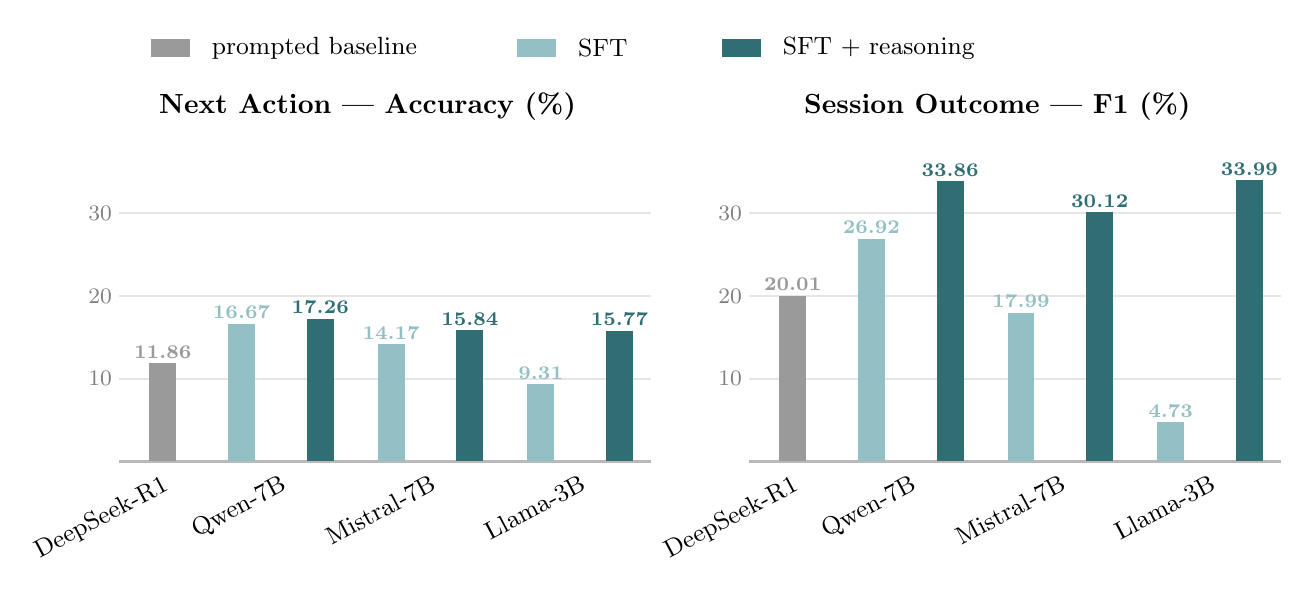
\begin{tikzpicture}[
      vlabel/.style={font=\scriptsize\bfseries,anchor=south,inner sep=1.6pt},
      xlab/.style={font=\small,anchor=north east,rotate=28,text=black,inner sep=1pt},
      yscale=0.105,
    ]
    \def\PB{8.0}
    \def\sep{0.5}
    \def\bw{0.17}
    \def\bx{0.7}
    \def\ga{2.2}\def\gb{4.1}\def\gc{6.0}
    \def\ly{50}
    \fill[barbase] (0.55,\ly-1.1) rectangle (1.05,\ly+1.1);
    \node[anchor=west,font=\small] at (1.2,\ly) {prompted baseline};
    \fill[barsft] (5.2,\ly-1.1) rectangle (5.7,\ly+1.1);
    \node[anchor=west,font=\small] at (5.85,\ly) {SFT};
    \fill[barpos] (7.8,\ly-1.1) rectangle (8.3,\ly+1.1);
    \node[anchor=west,font=\small] at (8.45,\ly) {SFT + reasoning};
    \begin{scope}
      \node[font=\bfseries,anchor=south] at (3.3,40) {Next Action \textemdash\ Accuracy (\%)};
      \foreach \g in {10,20,30}{
        \draw[gridln,line width=0.7pt] (0.15,\g) -- (6.9,\g);
        \node[font=\footnotesize,text=gray,anchor=east,inner sep=2.5pt] at (0.15,\g) {\g};
      }
      \draw[gray!55,line width=1pt] (0.15,0) -- (6.9,0);
      \fill[barbase] (\bx-\bw,0) rectangle (\bx+\bw,11.86);
      \node[vlabel,text=barbase] at (\bx,11.86) {11.86};
      \foreach \cx/\sv/\pv in {\ga/16.67/17.26, \gb/14.17/15.84, \gc/9.31/15.77}{
        \fill[barsft] (\cx-\sep-\bw,0) rectangle (\cx-\sep+\bw,\sv);
        \node[vlabel,text=barsft] at (\cx-\sep,\sv) {\sv};
        \fill[barpos] (\cx+\sep-\bw,0) rectangle (\cx+\sep+\bw,\pv);
        \node[vlabel,text=barpos] at (\cx+\sep,\pv) {\pv};
      }
      \node[xlab] at (\bx,-1) {DeepSeek-R1};
      \node[xlab] at (\ga,-1) {Qwen-7B};
      \node[xlab] at (\gb,-1) {Mistral-7B};
      \node[xlab] at (\gc,-1) {Llama-3B};
    \end{scope}
    \begin{scope}[shift={(\PB,0)}]
      \node[font=\bfseries,anchor=south] at (3.3,40) {Session Outcome \textemdash\ F1 (\%)};
      \foreach \g in {10,20,30}{
        \draw[gridln,line width=0.7pt] (0.15,\g) -- (6.9,\g);
        \node[font=\footnotesize,text=gray,anchor=east,inner sep=2.5pt] at (0.15,\g) {\g};
      }
      \draw[gray!55,line width=1pt] (0.15,0) -- (6.9,0);
      \fill[barbase] (\bx-\bw,0) rectangle (\bx+\bw,20.01);
      \node[vlabel,text=barbase] at (\bx,20.01) {20.01};
      \foreach \cx/\sv/\pv in {\ga/26.92/33.86, \gb/17.99/30.12, \gc/4.73/33.99}{
        \fill[barsft] (\cx-\sep-\bw,0) rectangle (\cx-\sep+\bw,\sv);
        \node[vlabel,text=barsft] at (\cx-\sep,\sv) {\sv};
        \fill[barpos] (\cx+\sep-\bw,0) rectangle (\cx+\sep+\bw,\pv);
        \node[vlabel,text=barpos] at (\cx+\sep,\pv) {\pv};
      }
      \node[xlab] at (\bx,-1) {DeepSeek-R1};
      \node[xlab] at (\ga,-1) {Qwen-7B};
      \node[xlab] at (\gb,-1) {Mistral-7B};
      \node[xlab] at (\gc,-1) {Llama-3B};
    \end{scope}
  \end{tikzpicture}}

  \vspace{2pt}
  \centering {\small \textbf{Prompting is not all you need:} small fine-tuned models beat the best prompted model, and synthesized \emph{reasoning} lifts outcome F1 further.}
\end{frame}

\begin{frame}{Results -- Distribution}
  \begin{figure}
    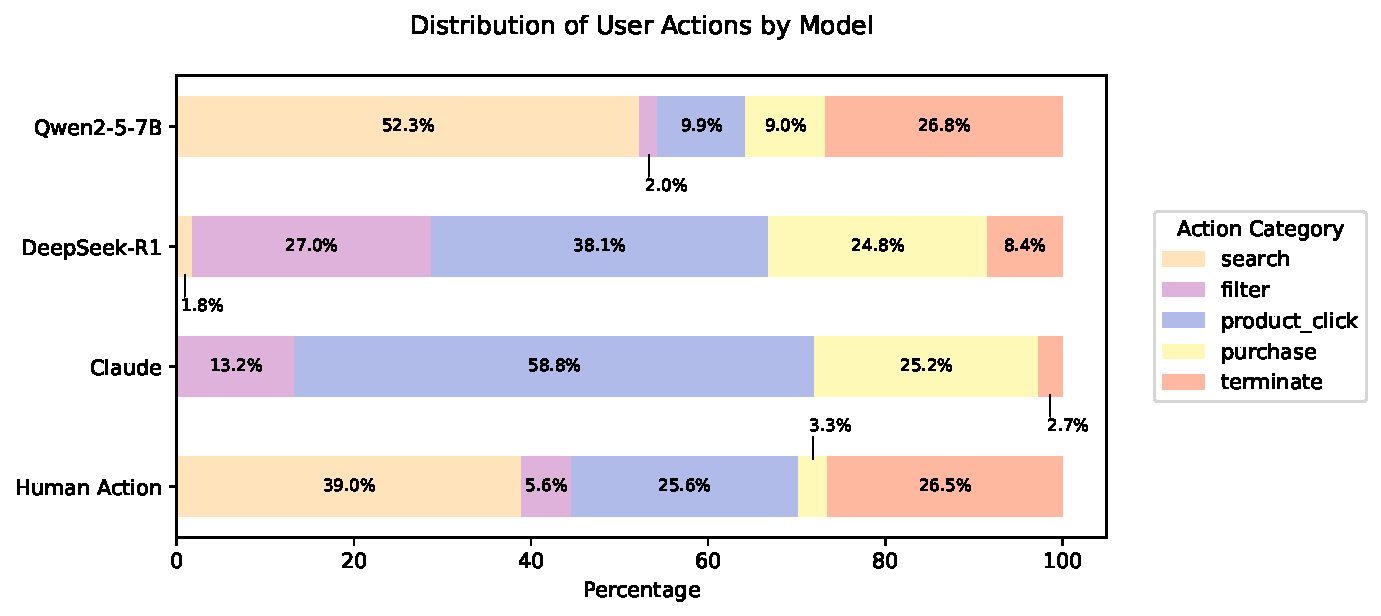
\includegraphics[width=\linewidth]{figures/finetuned_web_agent/action_distribution_below_labels.pdf}
    \caption{Distribution of the action types in the dataset.}
  \end{figure}
\end{frame}

% \begin{frame}{Ablation Study}
%   \begin{outline}
%     \1 To evaluate the impact of training model with synthesized reasoning trace, we conduct an ablation study \textbf{to remove the reasoning trace} from the training data.

%   \end{outline}
%   \begin{table}[t]
%     \centering
%     \begin{booktabs}{
%       colspec = {X[l]cc},
%       cells={m},
%       cell{3,5,7}{1}={r,font=\itshape},
%     }
%     \toprule
%     Model                         & { Action Gen. \\\ (Acc.) }& {Outcome \\ (F1)} \\
%     \midrule 
%     Qwen2.5-7B SFT                    & \textbf{17.26\% }            & 33.86\%            \\
%     w/o reasoning                 & 16.67\%             & 26.92\%            \\
%     Mistral-7Bv0.3 SFT               & 15.84\%             & 30.12\%            \\
%     w/o reasoning                 & 14.17\%             & 17.99\%            \\
%     Llama-3.2-3B SFT                  & 15.77\%             & \textbf{33.99\%}            \\
%     w/o reasoning                 & 9.31\%              & 4.73\%             \\
%     \bottomrule
%     \end{booktabs}
%     \caption{Ablation study result.}
%     \label{tab:ablation}
%     \end{table}
% \end{frame}

% \begin{frame}{Error Analysis}
%   \begin{outline}
%     \1 We analyze the errors made by the models: Claude and Qwen 2.5 7B.
%     \1 Error types\footnote{Illegal actions generated by models are excluded from this analysis.}:
%       \2 Didn't terminate
%       \2 Didn't click
%       \2 Didn't search
%       \2 Searched wrong keyword
%       \2 Clicked wrong button
%   \end{outline}
% \end{frame}

% \begin{frame}{Error Analysis}
%   \begin{figure}
%     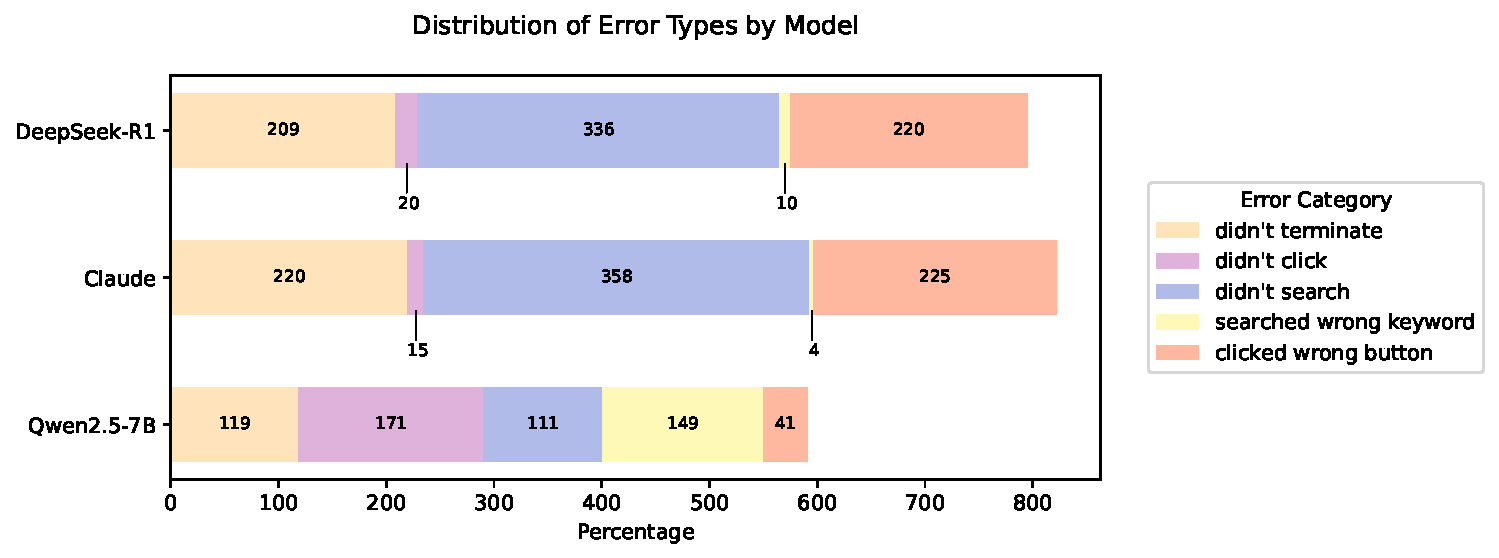
\includegraphics[width=\linewidth]{figures/finetuned_web_agent/error_analysis.pdf}
%     \caption{Error analysis.}
%   \end{figure}
% \end{frame}

% \section{Conclusion}

% \begin{frame}{Conclusion}
%   \begin{outline}
%     \1 We present the first quantative, process-centric evaluation of LLMs for simulating human behavior in online shopping.
%     \1 State-of-the-art models cannot simulate human behavior accurately, i.e. \textit{Prompting is not all-you-need!}
%     \1 Fine-tuning with reasoning traces significantly improves the accuracy of LLMs in simulating human behavior.
%   \end{outline}
% \end{frame}



\iffalse  
\begin{frame}[c]
  Supervised fine-tuning improves simulation accuracy, but it remains fundamentally limited.

  As an off-policy learning paradigm, SFT can only reproduce behaviors present in offline data or teacher-generated traces, rather than explore and learn new strategies.

  This places an inherent ceiling on performance.

  Beyond supervised fine-tuning, how can reinforcement learning further improve LLMs for human behavior simulation?
\end{frame}

% === WebServ (RL) section — presented by co-speaker; excluded from this deck ===
\section[WebServ: Browser-Server Environment for RL Web Agents]{WebServ: A Browser-Server Environment for Efficient Training of Reinforcement Learning-based Web Agents at Scale}


\begin{frame}{Web Browsers are NOT RL-Ready}
  \begin{outline}
    \1 Web Browsers are NOT RL-Ready:
      \2 Requires per-site configuration or rely on site features
      \2 Noisy context and action
  \end{outline}
\end{frame}

\begin{frame}{Web Servers are NOT RL-Ready}
  \begin{outline}
    \1 Web Servers are NOT RL-Ready
      \2 Expensive, slow, large image size
      \2 Single agent per server (lack of isolation)
      \2 Rollout is expensive
  \end{outline}
\end{frame}

\begin{frame}{System Architecture}
  % \begin{columns}[c]
  %   \begin{column}{0.48\linewidth}
  %     \textbf{Isolation vs. scalability.} Existing web environments rely on a shared server container that leads to cross-agent interference; \projectname creates lightweight per-agent containers to ensure isolation and scalable rollouts for RL training.
  %   \end{column}
  %   \begin{column}{0.52\linewidth}
      \begin{figure}
        
\includegraphics[width=.45\linewidth]{figures/webserv/teaser.png}
        % \caption{System architecture of \projectname.}
      \end{figure}
  %   \end{column}
  % \end{columns}
\end{frame}

% \begin{frame}{Observation Space}
%   \begin{outline}
%     \1 Observation Space: Compact, site-agnostic, generated from webpage DOM.
%       \2 Remove invisible or irrelevant nodes.
%       \2 Preserve interactivity cues (cursor styles).
%       \2 Provide stable, semantically meaningful IDs.
%   \end{outline}
% \end{frame}

% \begin{frame}{Action Space}
%   \begin{outline}
%     \1 Action Space: Minimal, human-aligned operations.
%       \2 Click, type\_and\_submit, select, etc.
%       \2 Simple parameters pointing to IDs.
%   \end{outline}
% \end{frame}

% \begin{frame}{Action Execution}
%   \begin{outline}
%     \1 Robust action executor for SPAs.
%       \2 Network-aware waiting until page settles.
%       \2 Generalizes across sites.
%   \end{outline}
% \end{frame}

% \begin{frame}{Server Stack}
%   \begin{outline}
%     \1 Incus-based manager with block-level COW.
%       \2 Fast launch, clone, reset.
%       \2 Works with existing Docker images.
%       \2 Supports 200+ concurrent containers on one host.
%   \end{outline}
% \end{frame}

\begin{frame}{Evaluation Highlights}
  \begin{outline}
    \1 \projectname + Claude 4.5: 40.0\% (Shopping), 62.9\% (CMS), 50.0\% (GitLab) on WebArena-Lite.
    \1 Faster spin-up: launch latency \textbf{$\sim$5$\times$} faster.
    \1 Storage: \textbf{$\sim$240$\times$} smaller persistent storage.
    \1 200+ concurrent containers on a single host.
  \end{outline}
\end{frame}

\begin{frame}{Benchmarks vs. Vanilla WebArena}
  \begin{table}[t]
    \centering
    \begin{booktabs}{
      colspec = {l l c c c},
      row{1} = {font=\bfseries}
    }
    \toprule
    Environment & Model & Shopping & CMS & GitLab \\
    \midrule
    Vanilla WebArena & GPT-4o       & 11.1 & 20.0 & 10.0 \\
    Vanilla WebArena & OpenAI-o3    & 33.3 & 45.7 & 46.7 \\
    Vanilla WebArena & Llama-3.1-8B & 8.9  & 5.7  & 10.0 \\
    \midrule
    \projectname & GPT-4o       & 20.0 & 28.6 & 43.3 \\
    \projectname & OpenAI-o3    & 37.8 & 48.6 & 46.7 \\
    \projectname & Llama-3.1-8B & 11.1 & 11.4 & 16.7 \\
    \bottomrule
    \end{booktabs}
    \caption{Single-prompt success rate (\%) on WebArena-Lite. \projectname lifts accuracy across proprietary and open-source models.}
  \end{table}
\end{frame}

% \begin{frame}{Ablation: Visual Cues}
%   \begin{table}[t]
%     \centering
%     \scriptsize
%     \begin{booktabs}{
%       colspec={lccc},
%       row{1}={font=\bfseries}
%     }
%     \toprule
%     Model & $\Delta$ Shopping & $\Delta$ CMS & $\Delta$ GitLab \\
%     \midrule
%     GPT-4o & \highlightRelevantValue{-33.3} & \highlightRelevantValue{-70.0} & \highlightRelevantValue{-46.2} \\
%     GPT-5 & \highlightRelevantValue{-18.8} & \highlightRelevantValue{-35.0} & \highlightRelevantValue{-25.0} \\
%     Claude 3.5 Sonnet & \highlightRelevantValue{-58.3} & \highlightRelevantValue{-45.5} & \highlightRelevantValue{-81.8} \\
%     Claude 3.7 Sonnet & \highlightRelevantValue{-50.0} & \highlightRelevantValue{-53.8} & \highlightRelevantValue{-66.7} \\
%     Claude 4 Sonnet & \highlightRelevantValue{-26.3} & \highlightRelevantValue{-29.4} & \highlightRelevantValue{-33.3} \\
%     Claude 4.5 Sonnet & \highlightRelevantValue{-5.6} & \highlightRelevantValue{-45.5} & \highlightRelevantValue{6.7} \\
%     \bottomrule
%     \end{booktabs}
%     \caption{Removing cursor/interaction visual cues hurts most models; weaker models drop more.}
%   \end{table}
% \end{frame}

% \begin{frame}{Ablation: Vision Signals}
%   \begin{table}[t]
%     \centering
%     \scriptsize
%     \begin{booktabs}{
%       colspec={lccc},
%       row{1}={font=\bfseries},
%       cell{3,5}{1}={r}
%     }
%     \toprule
%     Model & Shopping & CMS & GitLab \\
%     \midrule
%     Claude 4 Sonnet (text) & 42.2 & 48.6 & 50.0 \\
%     + VLM & 44.4 & 48.6 & 43.3 \\
%     Claude 4.5 Sonnet (text) & 40.0 & 62.9 & 50.0 \\
%     + VLM & 37.8 & 65.7 & 56.7 \\
%     \bottomrule
%     \end{booktabs}
%     \caption{Vision helps selectively; not universally beneficial across tasks.}
%   \end{table}
% \end{frame}

\begin{frame}{System Efficiency}
  \begin{table}[t]
    \centering
    \begin{booktabs}{
      colspec = {l c c},
      row{1} = {font=\bfseries}
    }
    \toprule
    Metric & \projectname (Incus) & Naïve Docker \\
    \midrule
    Launch speed & 1.781\,s & 8.963\,s \\
    Storage & 28.01\,MiB & 6.78\,GiB \\
    Memory & 1.74\,GiB & 1.63\,GiB \\
    \bottomrule
    \end{booktabs}
    \caption{Incus-based containers cut launch latency ($\sim$5$\times$) and storage ($\sim$240$\times$) at similar RAM.}
  \end{table}
\end{frame}
\fi  % === end WebServ section ===


% \begin{frame}{Recap}
%   \begin{outline}
%     \1 Designing: UXAgent shows how LLM agents can support UX researchers before running costly human studies.
%     \1 Evaluating: real behavioral data shows that current agents are still far from faithfully simulating humans.
%     \1 Improving: WebServ provides the infrastructure needed to train and improve web agents with reinforcement learning.
%   \end{outline}
% \end{frame}

% \begin{frame}[plain]
%   \begin{figure}[htp]
%     \centering
%     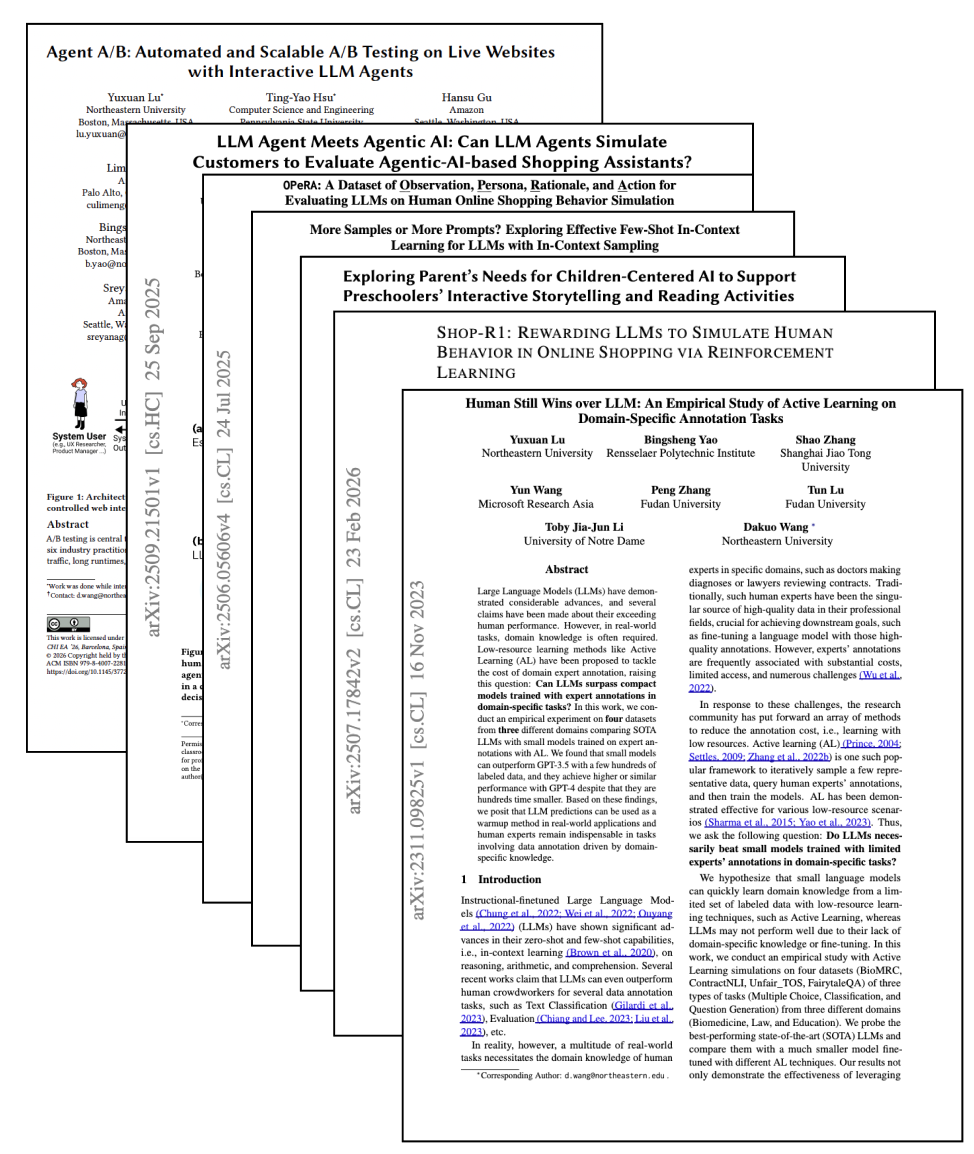
\includegraphics[height=\textheight]{papers.png}
%     % \caption{}
%   \end{figure}
% \end{frame}

\begin{frame}[standout]
  \Large Thank you!

  Questions?

  \begin{tikzpicture}[remember picture,overlay]
    \node[anchor=south east] at ([xshift=-0.8cm,yshift=0.8cm]current page.south east) {
      \qrcode[height=2cm]{https://yuxuan.lu}
    };
  \end{tikzpicture}
\end{frame}

\end{document}
